\documentclass[12pt]{article}

\usepackage{times,fullpage,xspace,fancyhdr,url,color}
\usepackage[pdftex]{graphicx}
\usepackage[pdftex,
            colorlinks=true,
            urlcolor=black,
            linkcolor=black,
            citecolor=black,
            bookmarksopen=false,
            bookmarksnumbered=true,
            pdfstartview=FitH]{hyperref}

\pdfcompresslevel=9
\newcommand{\leaguename}{RoboCup Standard Platform League (NAO) }
\hypersetup{
 pdftitle={\leaguename Rule Book},
 pdfauthor={Technical Committee SPL},
}
\usepackage{microtype}
\usepackage[utf8]{inputenc}
\usepackage{amsmath}
\usepackage{xargs}
\usepackage[colorinlistoftodos,prependcaption,textsize=tiny]{todonotes}
\usepackage{siunitx}
\usepackage[official]{eurosym}
\usepackage[useregional]{datetime2}
\DTMlangsetup[en-GB]{ord=raise,monthyearsep={,\space}}

\newcommandx{\unsure}[2][1=]{\todo[linecolor=red,backgroundcolor=red!25,bordercolor=red,#1]{#2}}
\newcommandx{\change}[2][1=]{\todo[linecolor=blue,backgroundcolor=blue!25,bordercolor=blue,#1]{#2}}
\newcommandx{\info}[2][1=]{\todo[linecolor=green,backgroundcolor=green!25,bordercolor=green,#1]{#2}}
\newcommandx{\improvement}[2][1=]{\todo[linecolor=Plum,backgroundcolor=Plum!25,bordercolor=Plum,#1]{#2}}

% comment 'disable' in to disable all the todo notes :)
\usepackage
[
%disable
]{todonotes}

\newcommand{\TotalWidth}{7.4}
\newcommand{\TotalLength}{10.4}
\newcommand{\GoalScoredDelay}{15 seconds\xspace}
\newcommand{\KickOffAutoTime}{45 seconds\xspace}
\newcommand{\KickOffBallFreeTime}{10 seconds\xspace}
\newcommand{\FreeKickTime}{30}
\newcommand{\FreeKickRadius}{0.75m\xspace}
\newcommand{\PlayingDelayTime}{15}
\newcommand{\PenaltyFreeKickTime}{30}
\newcommand{\PenaltyFreeKickSetupTime}{30}
\newcommand{\PenaltyKickTime}{30 seconds\xspace}
\newcommand{\StandardPenaltyTime}{45}
\newcommand{\StandardPenaltyIncrease}{10 seconds\xspace}
\newcommand{\NovelContributionTime}{3 years\xspace}
\newcommand{\GameStuckTime}{30}

\sloppy
\newcommand{\ie}{\mbox{i.\,e.}\xspace}
\newcommand{\eg}{\mbox{e.\,g.}\xspace}
%\newcommand{\cf}{\mbox{cf.}\xspace}
\newcommand{\cf}{see\xspace}
\newcommand{\comment}[1]{\marginpar{\pdfannot width 4in height .5in depth 8pt {/Subtype /Text /Contents (#1)}}}
\newcommand{\inparagraph}[1]{\paragraph{#1\hspace{-1em} }}


% some colors
\definecolor{orange}{rgb}{1,0.5,0}
\definecolor{red}{rgb}{1,0,0}
\definecolor{green}{rgb}{0,1,0}


\title{\leaguename Rule Book}
\author{RoboCup Technical Committee}
\date{(DRAFT 2022 rules, as of \today)}

\setlength{\parindent}{0pt}
\setlength{\parskip}{12pt plus 6pt minus 3 pt}
\setcounter{tocdepth}{1}
\widowpenalty=10000
\clubpenalty=10000

\pagestyle{fancy}
\lhead{}
\chead{}
\rhead{}
\lfoot{}
\cfoot{}
\rfoot{}

\renewcommand{\headrulewidth}{0.4pt}
\renewcommand{\footrulewidth}{0.4pt}

% needed to align an image and text correctly side by side
\newcommand{\imagebox}[1]{\raisebox{2ex}{\raisebox{-\height}{#1}}}

\begin{document}

\maketitle

\begin{center}
Questions or comments on these rules should be mailed to \url{rc-spl-tc@lists.robocup.org}.
\end{center}

\newpage

\tableofcontents
\setcounter{tocdepth}{3}

\thispagestyle{fancy}

\clearpage

\cfoot{\thepage}
\setcounter{page}{1}

\newpage

% !TeX root = ../SPL-Rules.tex
% !TeX spellcheck = en_US
\section{Setup of the Environment}
\label{sec:setup_environment}

\subsection{Field Construction}
\label{sec:field_dim}

The standard soccer field consists of \qty{8}{\milli\metre} artificial turf mounted on a flat wooden base with a total area of length~\qty{\TotalLength}{\metre} and width~\qty{\TotalWidth}{\metre}. Care should be taken to ensure the field is as flat and level as possible. Additionally, the wooden base should be well-supported and should not give when humans stand or walk on it.

Figure~\ref{fig:field_dim} shows the dimensions of a standard soccer field.
A more detailed technical drawing is provided in Appendix~\ref{apx:technical-drawing} to this document.
Note that the penalty cross is a cross and there is a dash at center field. White field lines can be made of the same \qty{8}{\milli\metre} artificial turf, but in white (\ie, made of white artificial turf), spray-painted or taped. Regardless of the solution, the field lines must be durable throughout the competition.

Figure~\ref{fig:goal_dimensions} and Figure~\ref{fig:goal_appearance} depict the construction and placement of the goals. A support structure for the net shall be made with small black, white, or gray bars or cylinders.  The support structure shall be constructed exactly as shown in Figure \ref{fig:goal_appearance}.

\begin{figure}[b!]
\centering
\centerline{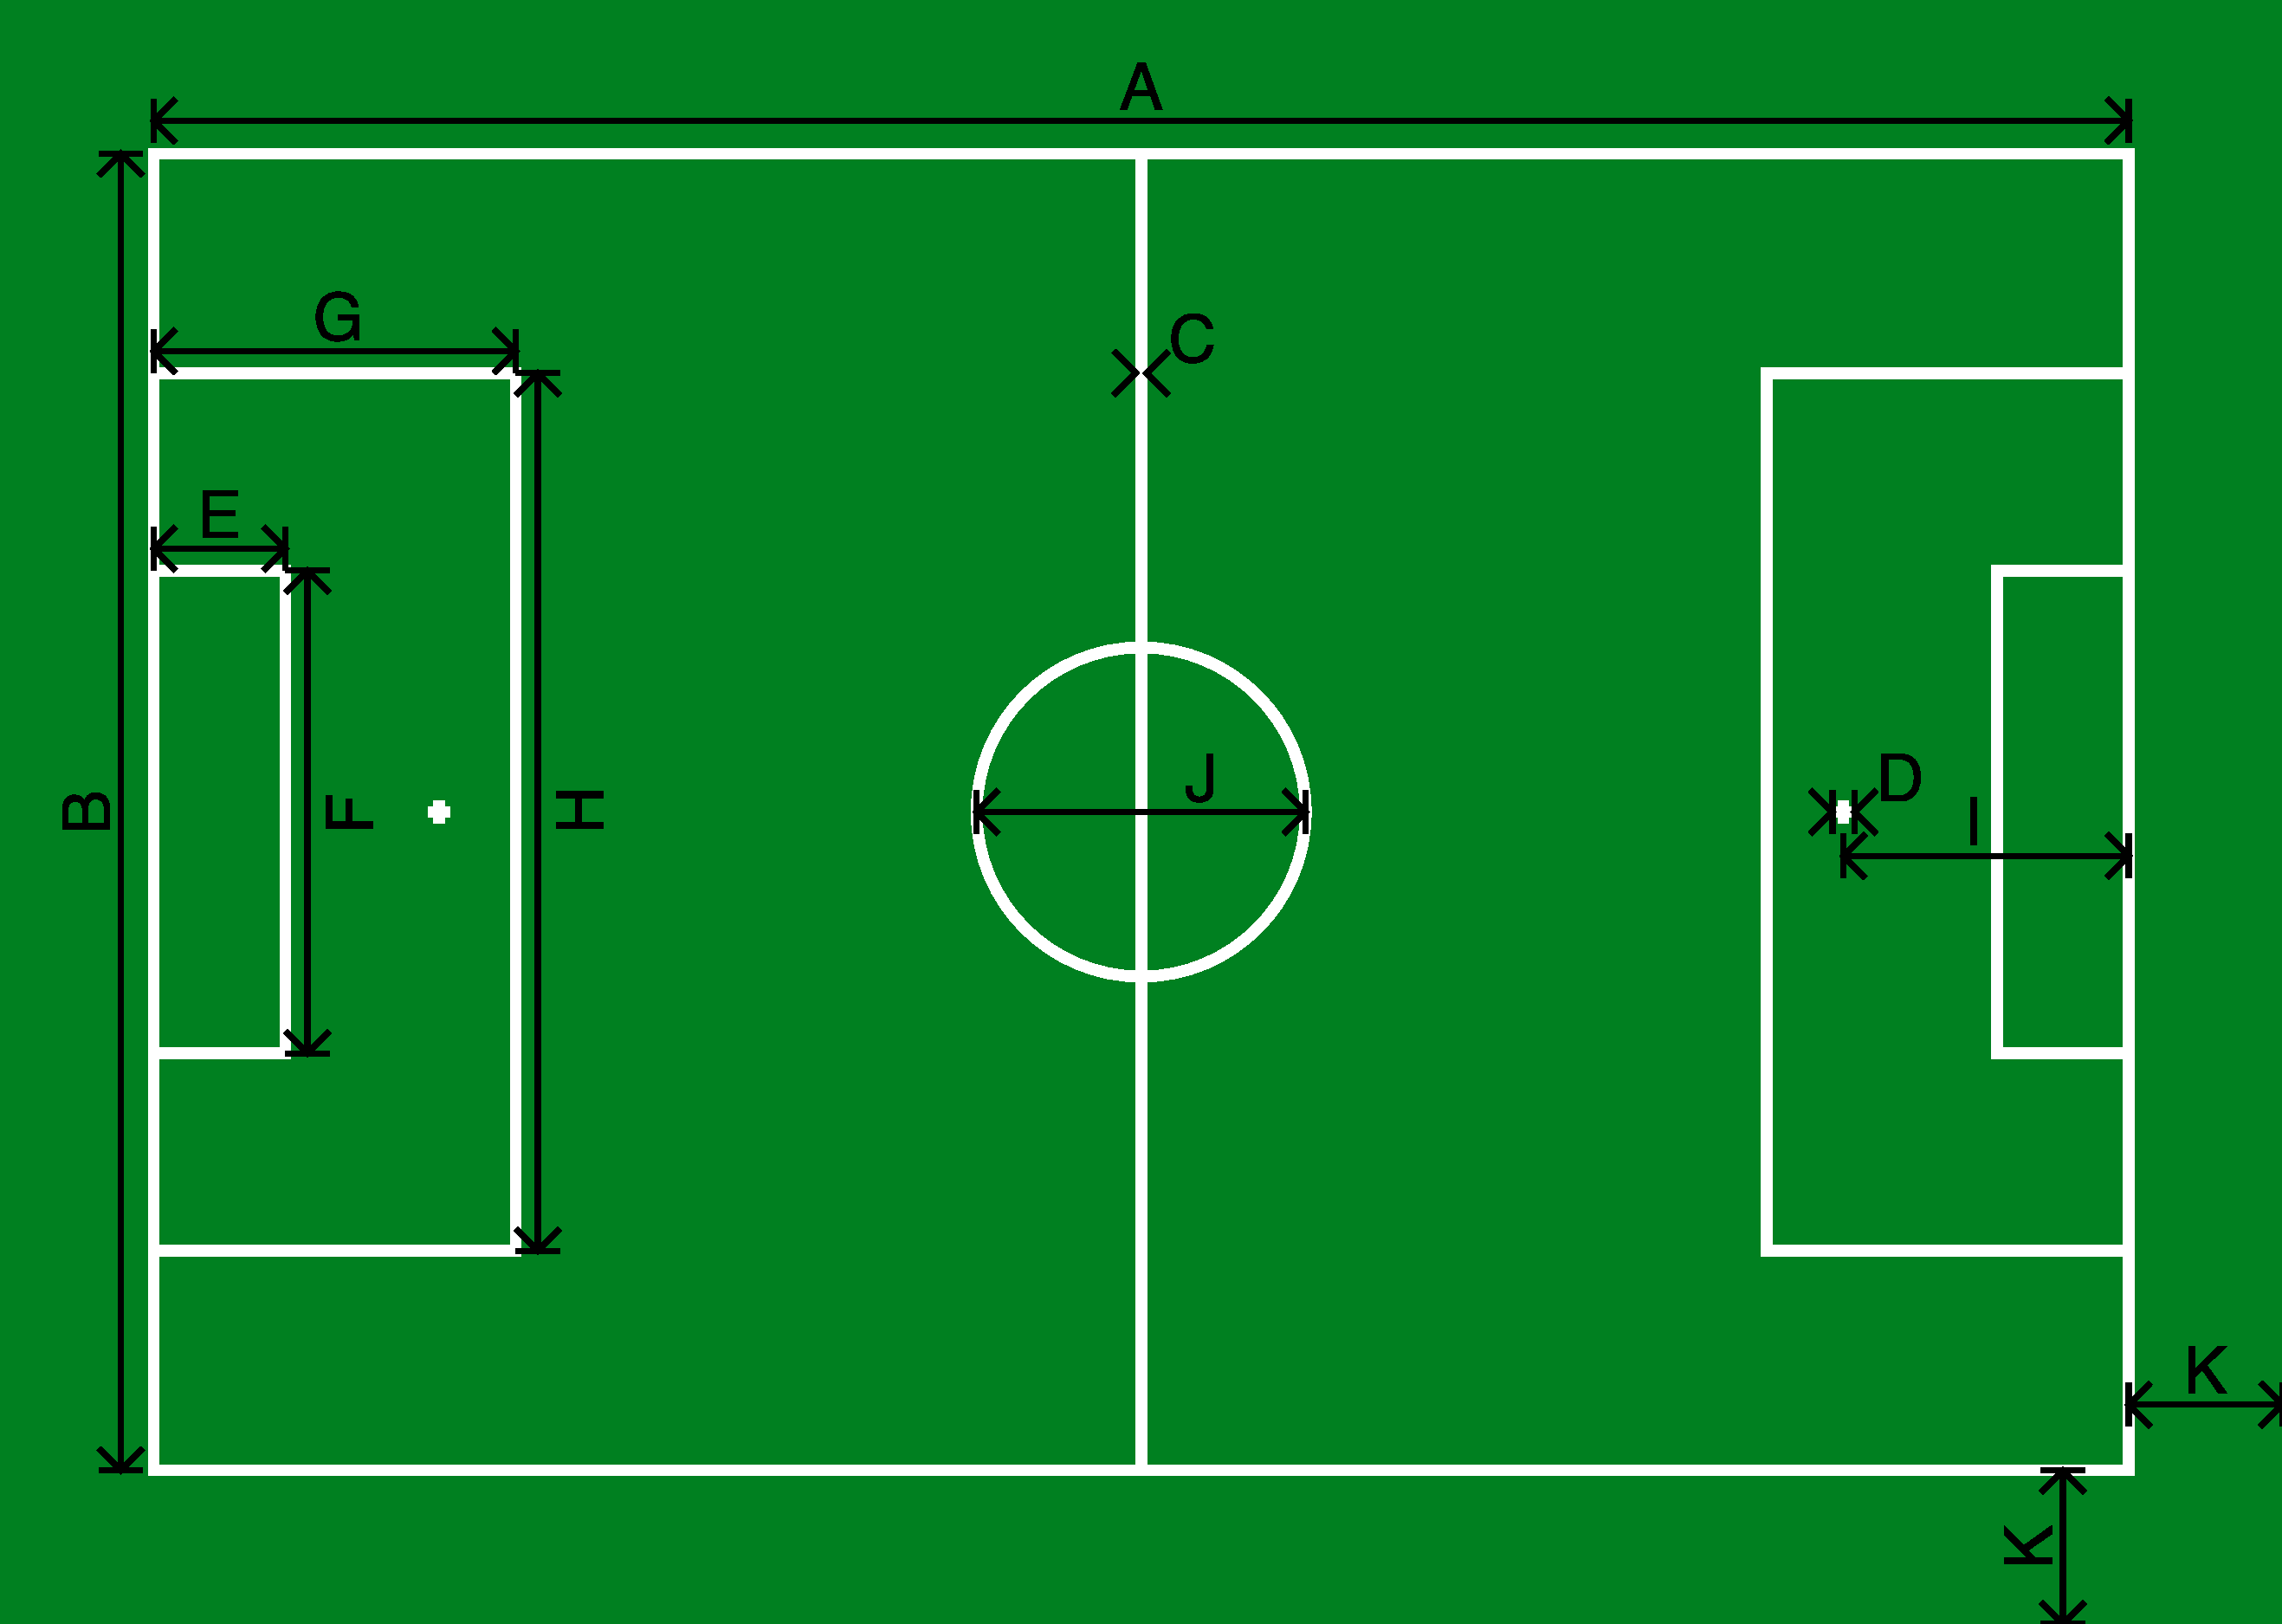
\includegraphics[width=\columnwidth]{figs/fieldDimensions2020.pdf}}
\vspace{1ex}
\begin{tabular}{| l | l | l |}
ID & Description & Length (in mm) \\
\hline \hline
A & Field length & 9000 \\
\hline
B & Field width & 6000 \\
\hline
C & Line width & 50 \\
\hline
D & Penalty cross size & 100 \\
\hline
E & Goalbox area length & 600 \\
\hline
F & Goalbox area width & 2200 \\
\end{tabular}
\begin{tabular}{|l|l|l|}
ID & Description & Length (in mm) \\
\hline \hline
G & Penalty area length & 1650 \\
\hline
H & Penalty area width & 4000 \\
\hline
I & Penalty cross distance & 1300 \\
\hline
J & Center circle diameter & 1500 \\
\hline
K & Border strip width & 700 \\
\hline
 &  &  \\
\end{tabular}
\caption{Schematic diagram of the soccer field (not to scale) and corresponding dimensions in mm.  Note that measurements on this diagram are made to the center of lines.}
\label{fig:field_dim}
\end{figure}


\begin{figure}[t!]
\begin{center}
\leavevmode
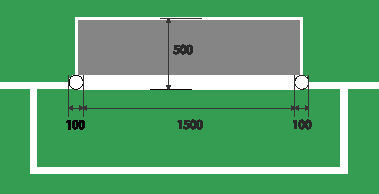
\includegraphics[width=1\columnwidth]{figs/goalDimensions2015.pdf}
\caption{Dimensions of the goal (in mm), viewed from above, and its placement on the field.}
\label{fig:goal_dimensions}
\end{center}
\end{figure}

\begin{figure}[h!]
\begin{center}
\leavevmode
\begin{minipage}[t]{0.49\columnwidth}
\imagebox{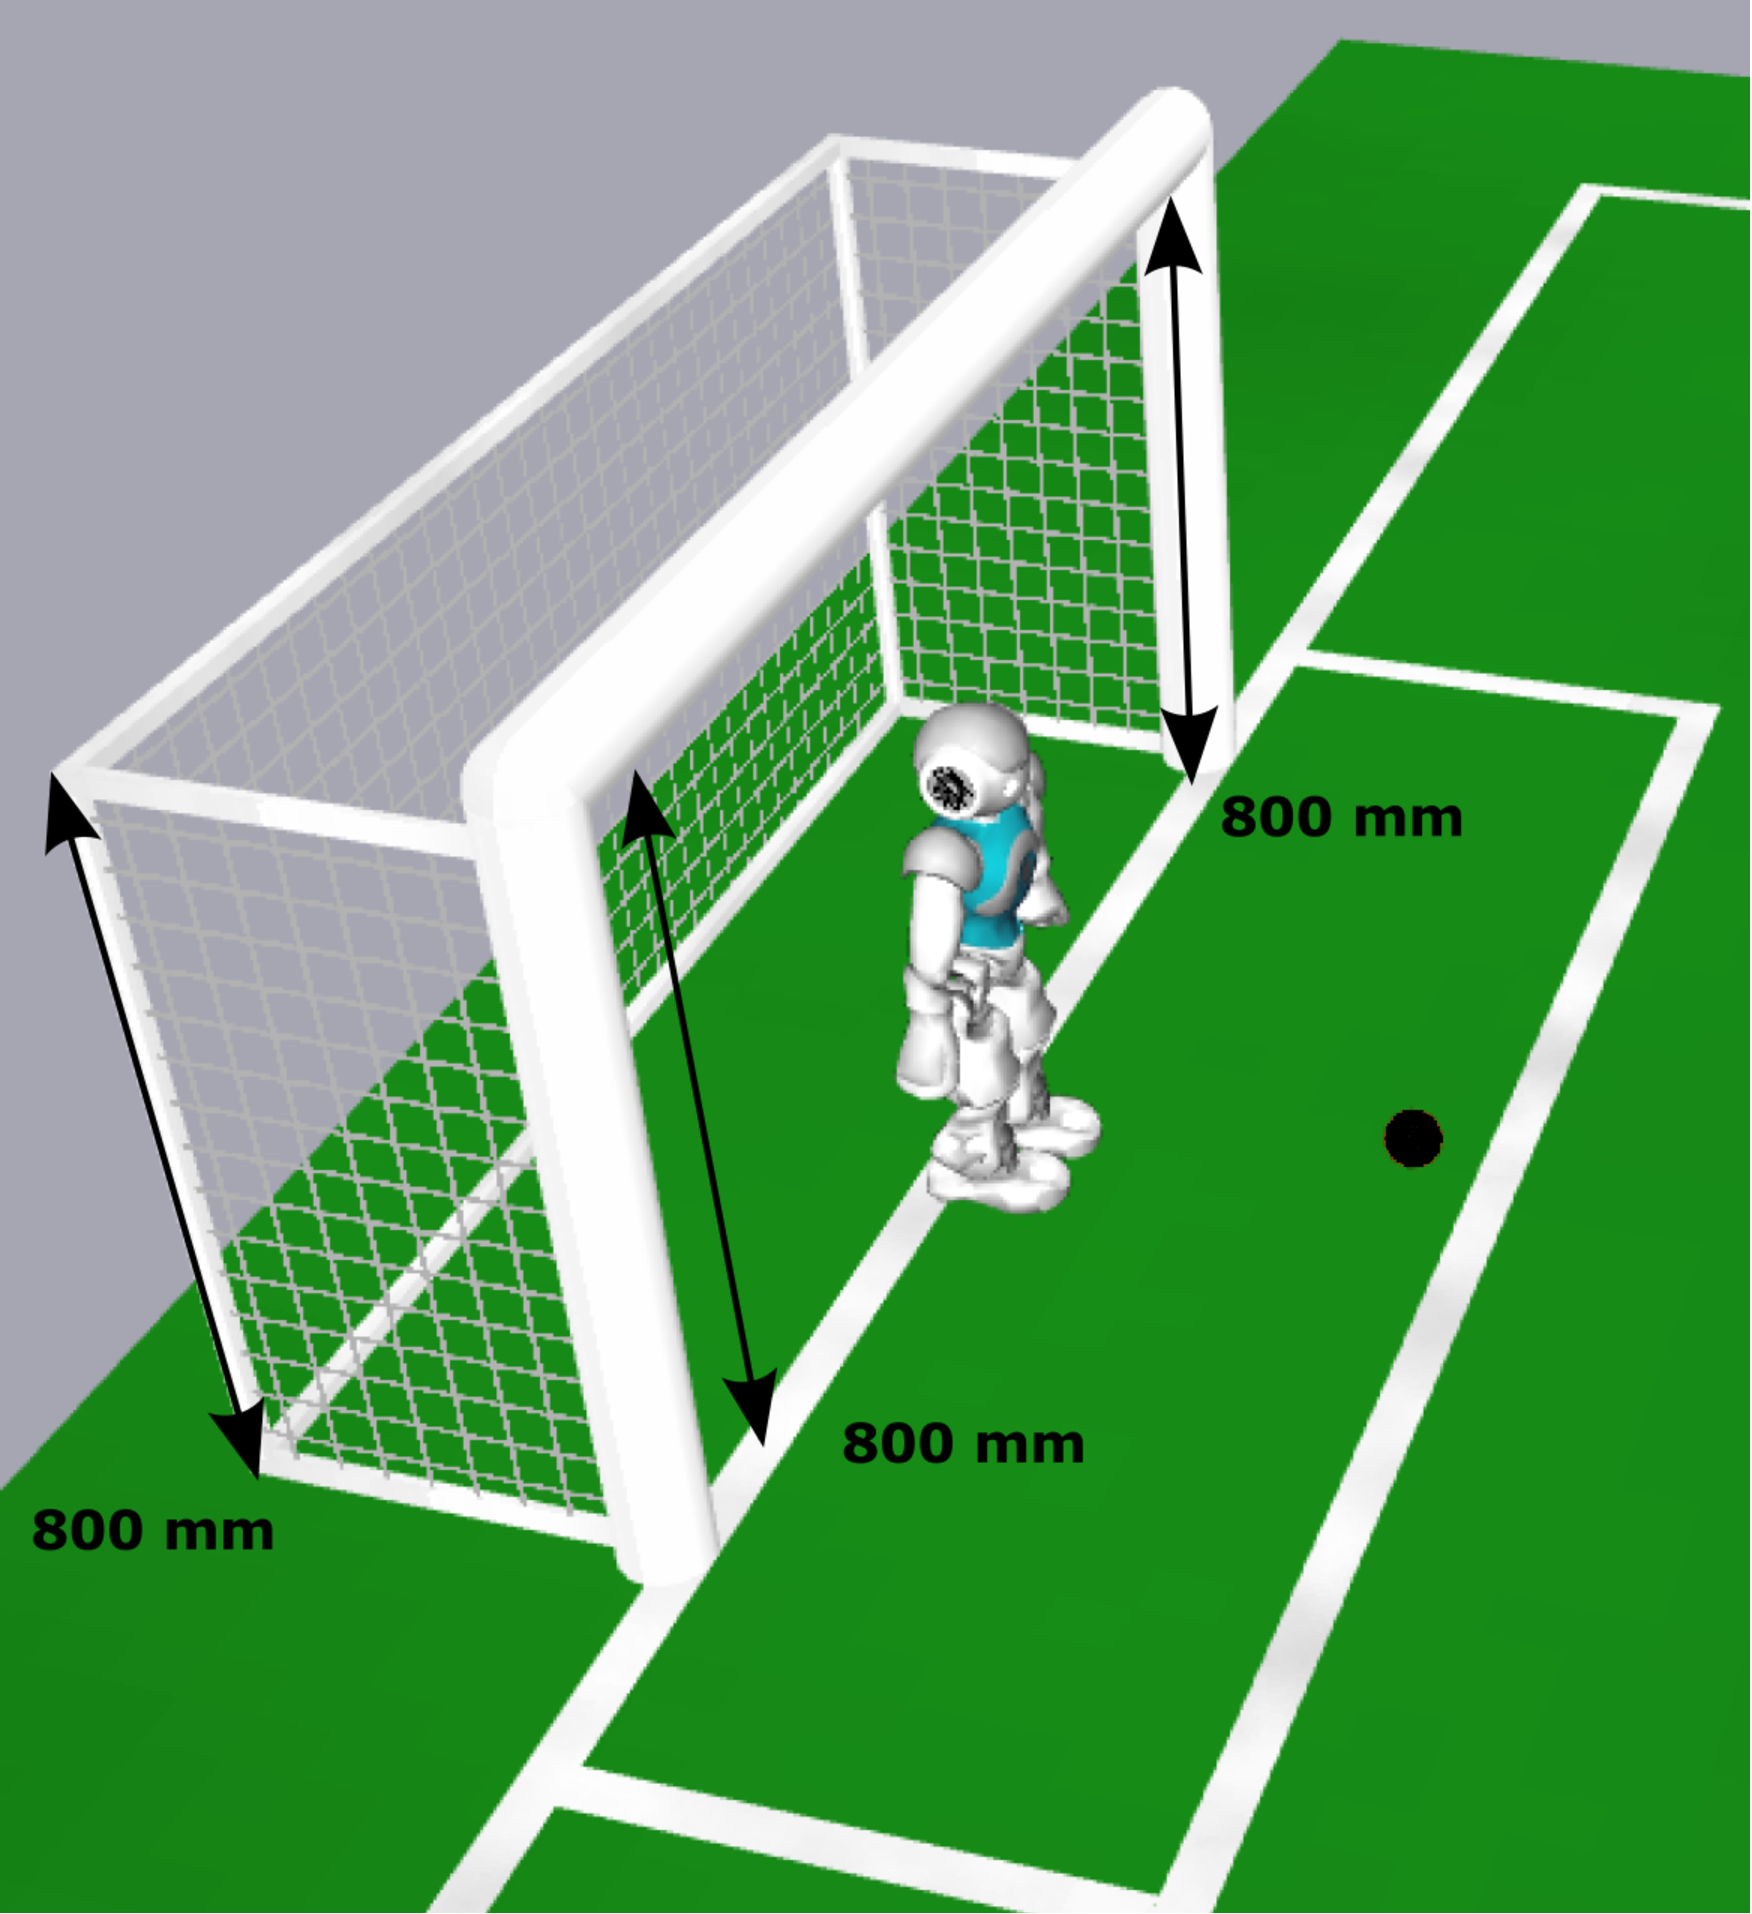
\includegraphics[width=1\columnwidth]{figs/goalDimensions3D.pdf}}%
\end{minipage}
\begin{minipage}[t]{0.49\columnwidth}
The goalposts and crossbar are made from 3 white cylinders with a diameter of \qty{100}{\milli\metre}.
The net:
\begin{itemize}
\item has a height of \qty{800}{\milli\metre}
\item is of white, gray or black color
\item is tightly supported via the support structure, in a way to minimize interference with the goal keeper
\item has a weave with holes smaller than the ball diameter.
\end{itemize}
\end{minipage}
\caption{Appearance and dimensions of the goals.}
\label{fig:goal_appearance}
\end{center}
\end{figure}

\subsection{Field Colors}
\label{sec:field_colors}
The colors of the soccer field are as follow:

\begin{itemize}

\item The field (artificial turf) itself is green (color is not specified, but it should not be too dark).

\item The lines on the field are white, whether they are taped, spray painted or made from white artificial turf.

\item Goals~(\cf Figure~\ref{fig:goal_appearance}). The posts and top crossbar of both goals are white. The net and the support structure for the net are white, gray, or black.

\end{itemize}

\subsection{Lighting Conditions}
\label{sec:lightConditions}
The lighting conditions depend on the actual venue. SPL fields should be placed near or under windows where possible. Whether window lighting is used, ceiling lights should be provided as necessary to ensure that most of the field is never darker than 300 Lux (400 Lux preferred).

Lighting is not required to be even and hotspots may occur on the field. The lighting design (comprising both natural and artificial light sources) shall aim to limit the ratio between the brightest and darkest patches on the field to less than 10:1. In general, lighting irregularities, including changes that occur during the competition, are acceptable and will not be cause for delay.  Such irregularities may include sun streaming through windows, light bulbs turning off, light bulbs being replaced, etc.

\subsection{Venue Setup}
\label{sec:boundaries}
Fields may be located close to one another.  Barriers will not necessarily be constructed between adjacent fields to block the robots from seeing other fields, goals, or balls. However, barriers will be constructed to block sight between any fields that are not located at least three meters apart. Hence, for each side of a field that is adjacent to another field, either barriers will separate the fields or at least \qty{3}{\metre} will be between the carpet of adjacent fields.

\subsection{Ball}
\label{sec:ball}

The official ball is a soft foam ball with a black and white soccer ball print (see Figure~\ref{fig:ball}). They are \qty{100}{\milli\metre} in diameter and weight \qty{44}{\gram}. These balls are available by writing to \url{info@sportpaint.de} (in German or English) and asking to order the "pu schaumstoffball 10cm 100ss".  Each ball costs \euro{2.0} plus shipping, where shipping cost depends on the destination.

\begin{figure}[t]
  \centerline{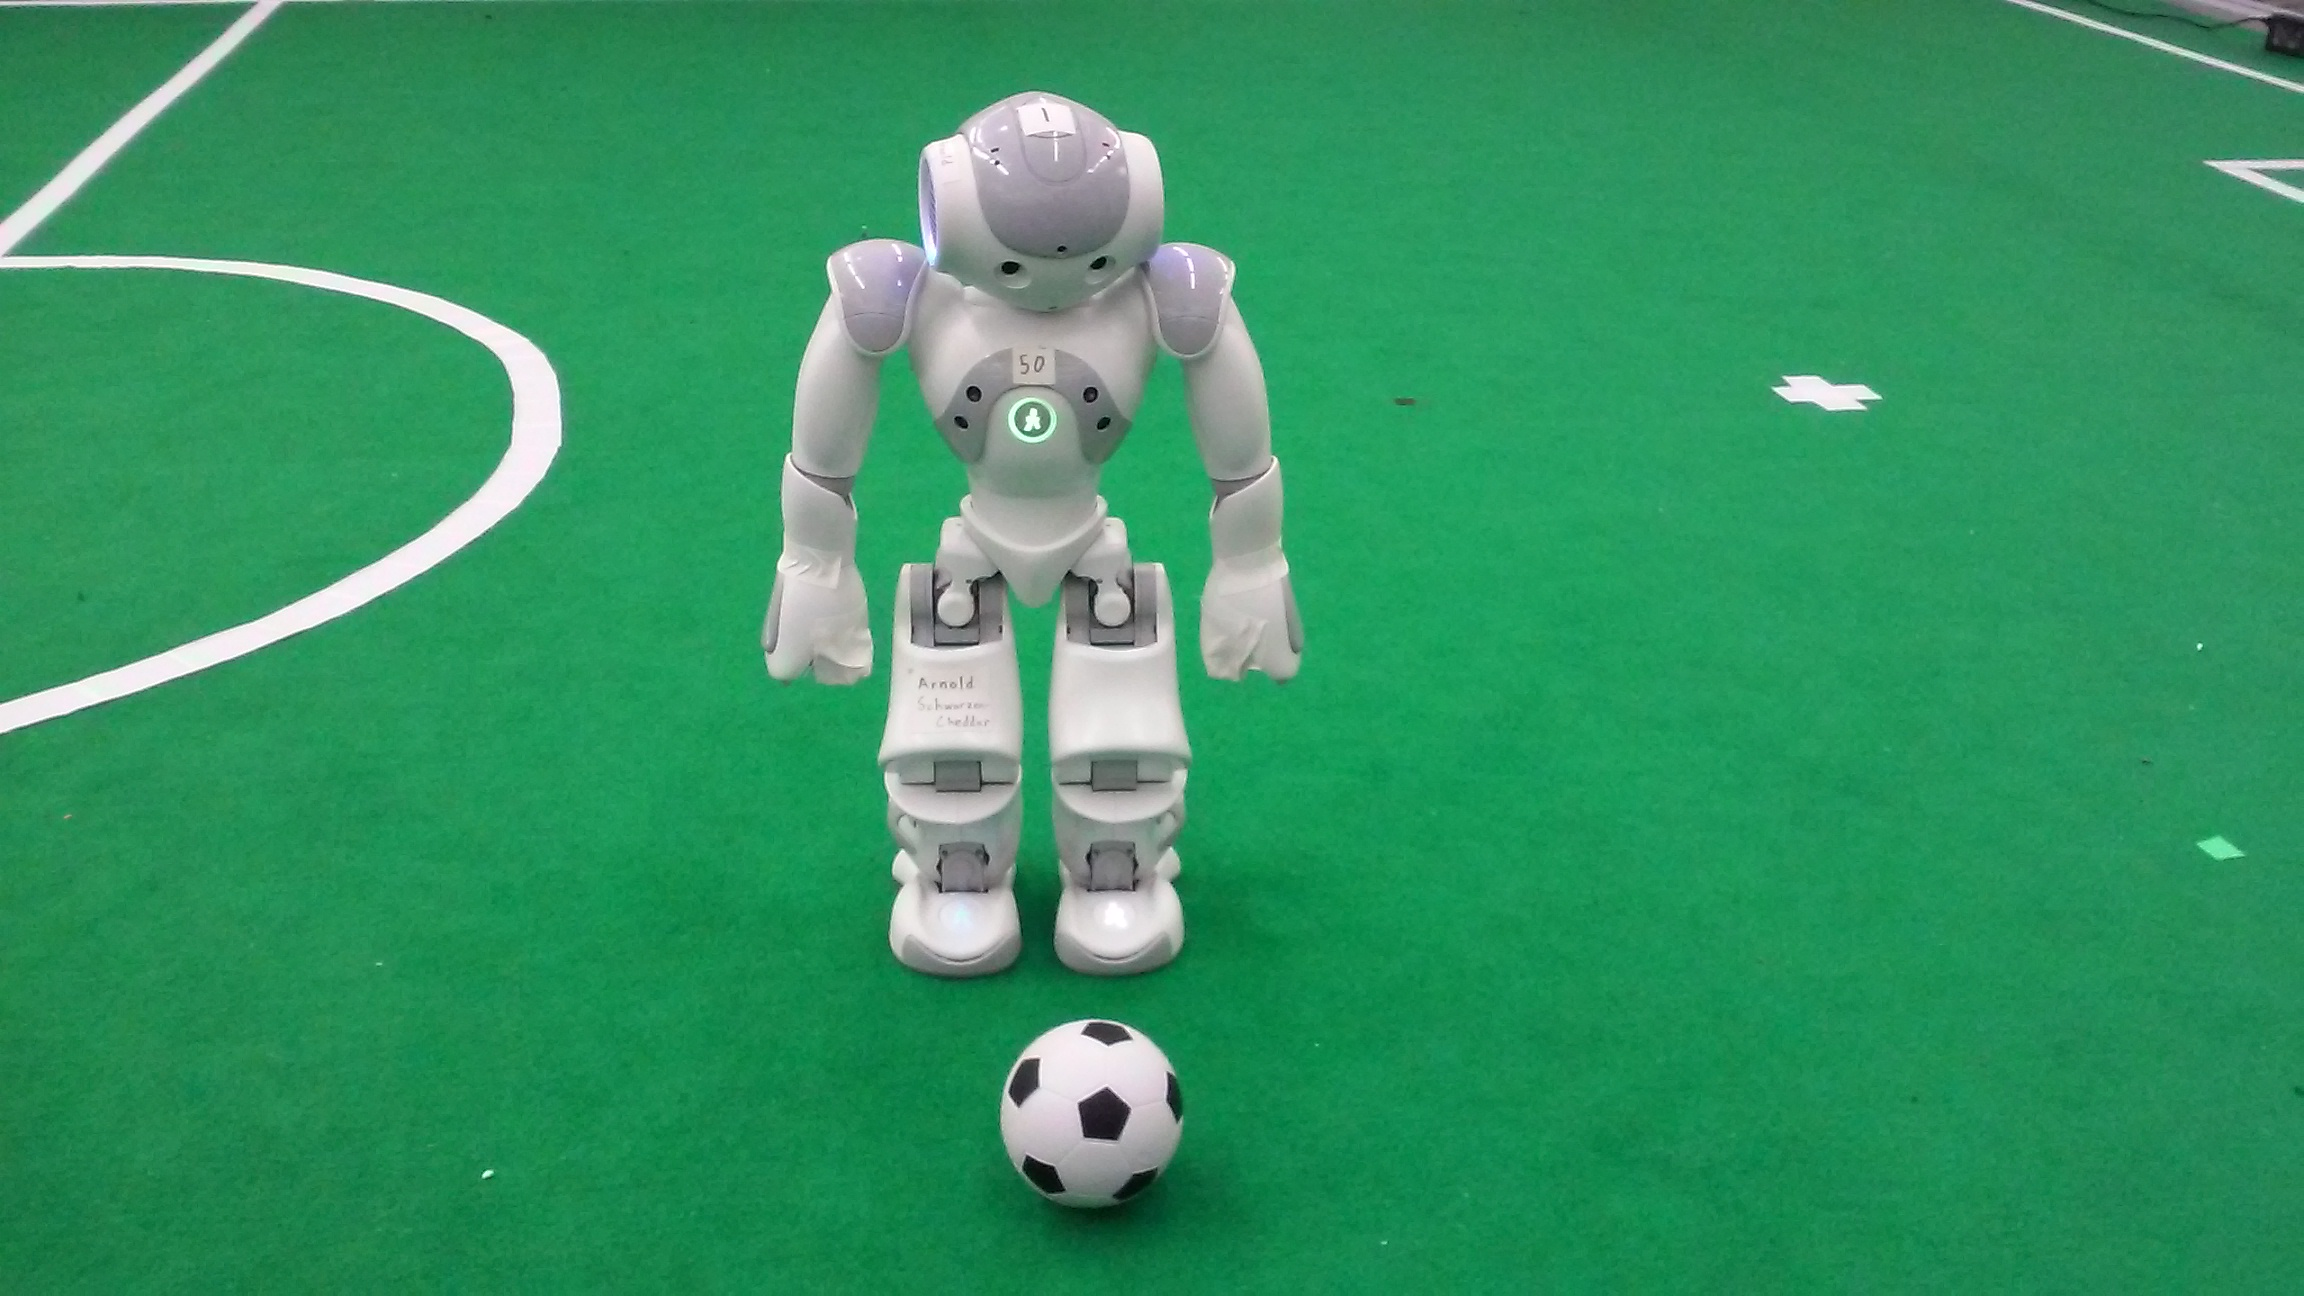
\includegraphics[height=0.28\columnwidth]{figs/robotWithBall2016.jpg}}
  \caption{A NAO and an official ball.}
  \label{fig:ball}
\end{figure}

\subsection{Definition of Inside and Outside}
\label{sec:inside_outside}

A line is always part of a region of the field.
This means, that \emph{inside/outside \textless region\textgreater} refers to the green area as well as the surrounding line.
Specifically:
\begin{itemize}
    \item The field boundary lines are part of the field
    \item The penalty box lines (and the end field line inside of the goal) part of the penalty box
    \item The center circle lines are part of the center circle
\end{itemize}

The only \textit{exception} to this rule is the center field line, which does not form part of any half.
That is, a robot is \textit{outside} a half of the field if it is touching the center line.

\subsection{Streaming setup}
\label{sec:streaming_setup}

There are multiple use cases for a streaming setup: 
\begin{itemize}
	\item Stream all videos to RoboCup SPL Youtube channel to store them there
	\item Allow team members from remote to watch their robot's match
	\item Evaluate team's performance measures online from videos recording (Part of Technical Challenge 2022)
\end{itemize}

A recommended streaming setup with all instruction for hardware, software and how to operate the setup can be found in this Github repository. \todo{Give link after dicussion with Arne}

\newpage

% !TeX root = ../SPL-Rules.tex
% !TeX spellcheck = en_US
\section{Robot Players}
\label{sec:robot_players}
A match is played by two teams, each consisting of not more than \textbf{5} players. At most one player may be designated as \emph{goalkeeper}, the others are all \emph{field players}.

\subsection{Hardware}
\label{sec:hardware}
All teams must use black, gray, red, blue, or orange plated NAO humanoid robots manufactured by SoftBank Robotics.

Absolutely no modifications or additions to the robot hardware are allowed. No additional hardware is permitted including off-board sensing or processing systems. Additional sensors besides those originally installed on the robots are likewise not allowed. The only exceptions are:

\begin{itemize}
    \item Setting the passive wrist joints to a fixed position either with glue or a transparent or white duct tape.
    \item Protecting the fingers with white finger protectors provided by the manufacturer or with transparent or white duct tape.
    \item Placing white duct tape over the battery case and screw (under the robot jersey) to keep the battery case in place and prevent the battery becoming disconnected.
    \item A memory stick may remain in the head during operation.  Only ordinary USB flash memory keys that sit flush or recessed to the head casing may be utilized. Other USB dongles or devices, as well as memory sticks that are not flush or recessed, are not permitted.
\end{itemize}

A computer with two monitors (one for GC and one for TCM) will be provided by the event organizers for the purpose of sending GameController messages to the robots and observing if no robot violates the rules for WIFI usage.
Additionally, there should be at least one monitor mirroring the second screen of the GC PC with the TCM in visitor mode. \todo{Clearfy this, which TCM mode}

\subsection{Goal Keeper}
\label{sec:goal_keeper}

The goal keeper is allowed to touch the ball with its arms/hands only while it is within its own goal box area. It always has the jersey number ``1''.

\subsection{Field Players}
\label{sec:field_players}
Each of the four field players has a jersey number from the set $\{2, 3, 4, 5, 6\}$. However, by default, the number ``6'' should only be used for a substitute that enters the game later.

\subsection{Team Markers}
\label{sec:team_markers}

Robots use colored jersey shirts as team markers. Each jersey shirt has a player number (1-6) printed on it.  The team markers are worn as shown in Figure~\ref{fig:nao_markers}.

\begin{figure}
  \centerline{\begin{tabular}{lll}
      a) & b) & c) \\
      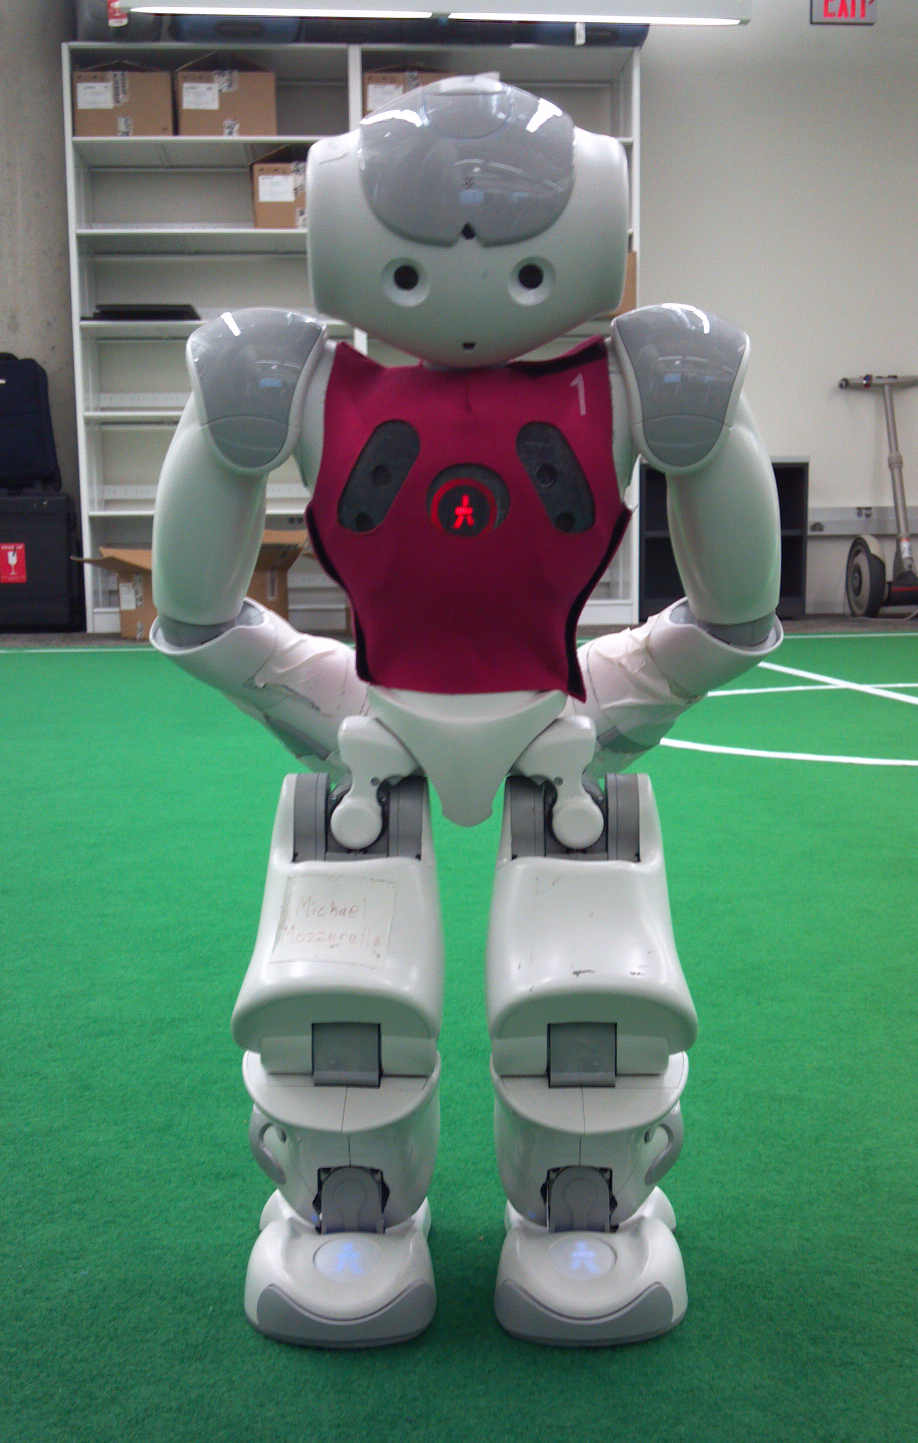
\includegraphics[height=0.28\columnwidth]{figs/front.jpg}&
      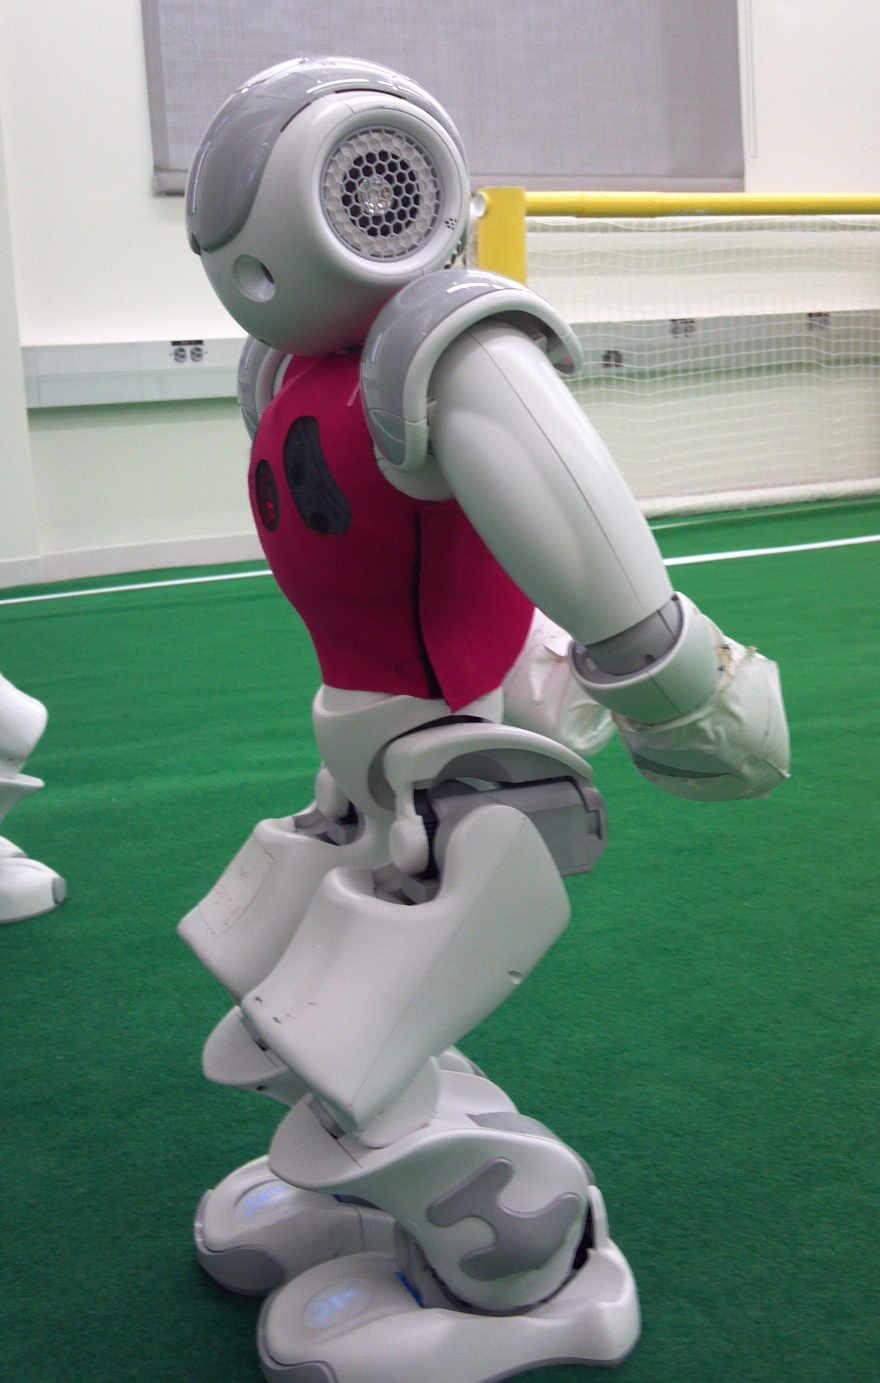
\includegraphics[height=0.28\columnwidth]{figs/side.jpg} &
      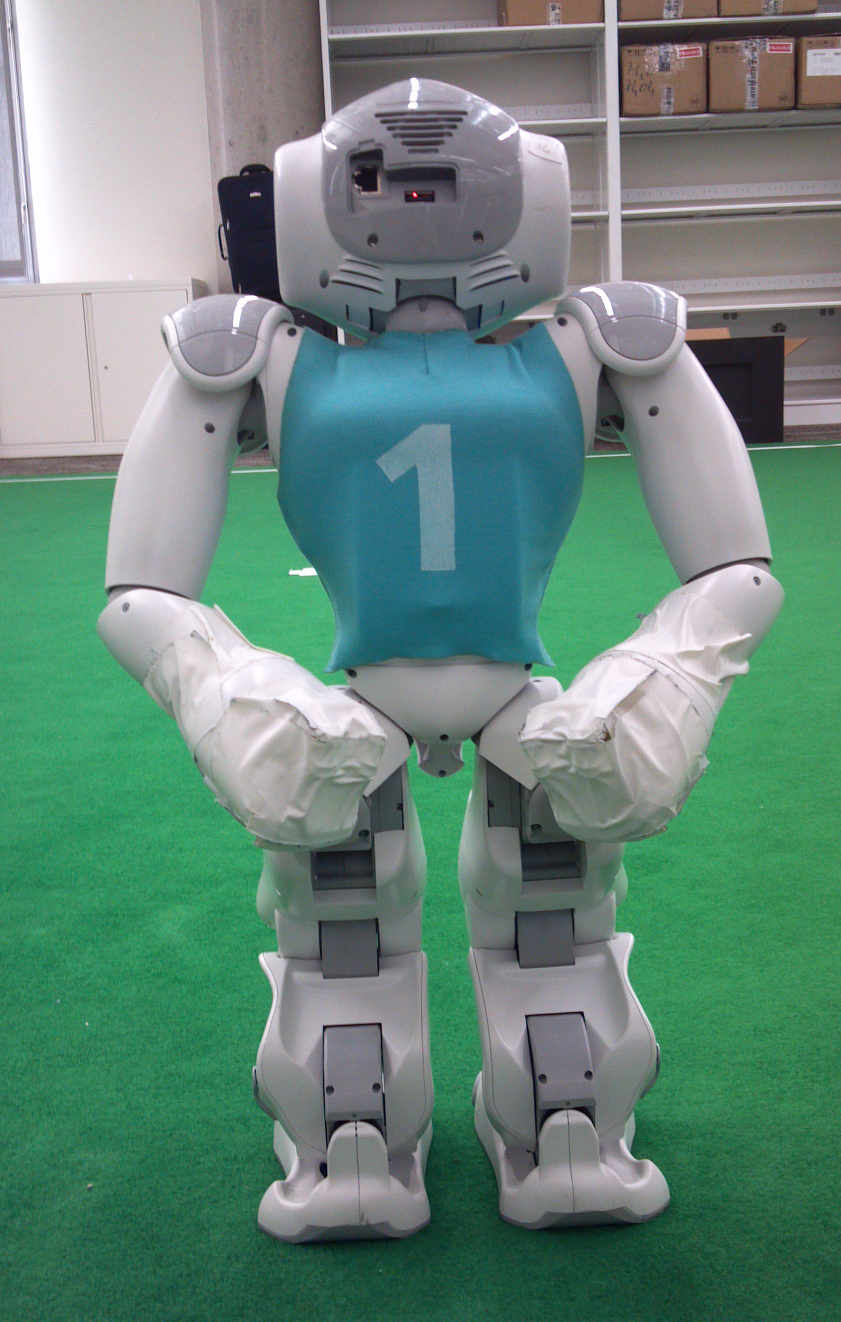
\includegraphics[height=0.28\columnwidth]{figs/back.jpg}
  \end{tabular} }
  \caption{Team markers. a) Front view. b) Side view. c) Back view.}
  \label{fig:nao_markers}
\end{figure}
Teams may use any jersey that was approved for a RoboCup SPL competition in the last 4 years without needing to reapprove it in 2022.\todo{Make parameter}

Teams may design and manufacture their own jerseys in any color (multi and many color jerseys are acceptable), but must follow these guidelines:
\begin{itemize}
\item Jerseys should be the \textbf{tank top} style used at RoboCup 2013/2014 and should cover approximately the same areas of the robot as shown in Figure~\ref{fig:nao_markers}. The torso LED must be clearly visible. Jerseys may include the sonar panel used in the 2013/2014 jerseys, although this is not required. Jerseys may not cover the shoulders of the robots.
\item Jerseys must have a primary color that comprises at least \qty{70}{\percent} of the jersey.
\item Jerseys should not contain distractors, such as large pictures of SPL balls or white stripes on green jerseys.
\item All players on a team must wear identical jerseys, including the goalkeeper.
\item A team must wear the jerseys that it starts a game in for the entire game.
\item Jersey material must be non-reflecting, non-shiny, and non-textured.  Material that is glittery is also not appropriate.
\item Jerseys should be numbered 1-6 on both sides.  The numbers must be large and {\bf easily} recognized by humans.
\item Teams must have two sets of jerseys that are significantly different in terms of their primary color.
\item Designs must be submitted to \url{rc-spl-tc@lists.robocup.org} for approval by \DTMdate{2022-05-01}.\todo{Make parameter} If the team has jersey prototypes, they should submit close-up images of a robot wearing the jersey — these images should be taken from front, back, and side angles.  If the team has no prototypes, then designs depicting the expected jersey should be submitted.  If submissions show separated front and back halves of jerseys then the team must specify which halves are matched to form home and away jerseys.  All images and designs should be submitted in pdf or jpg format.
\end{itemize}

Each team must designate a ``home'' color and an ``away'' color when asked about one month before RoboCup. Teams must wear their `home' jerseys when they are ```home'' (the first team listed on the schedule). Teams will wear their ``home'' jersey when they are ``away'' (the second team listed on the schedule) as well, unless either the head referee or the GameController program believes the jerseys of two competing teams are too similar.  In this case, the ``away'' team will then wear their ``away'' jersey.

Some teams wish to include additional information or logos on their robots. The following are allowable:

\begin{itemize}
  \item Attaching player numbers to the heads and/or legs of the robots. These numbers should be black with a white background, and should correspond to the number on the robot's jersey.

  \item Adding sponsor or team logos to the upper legs of the robots (\cf Figure~\ref{fig:sponsor}). A box drawn around the non-white area of these logos must not cover more than a \qty{25}{\square\centi\metre} area. At most one logo may be attached per leg - if you wish to attach more than one logo per leg, email the Technical Committee at least two weeks before the competition. Depending on the size and design of the logos, this may be allowable.

  \item Adding small black and white stickers to the torso of the robots stating the name of the robot, the name of the team, or similar information. These stickers must be small and mostly white.
\end{itemize}

\begin{figure}[b]
  \centerline{\begin{tabular}{ll}
  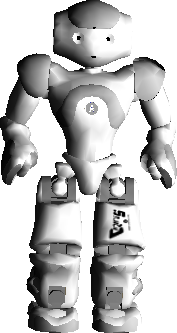
\includegraphics[height=0.35\columnwidth]{figs/naosim_with_logo.png}&
  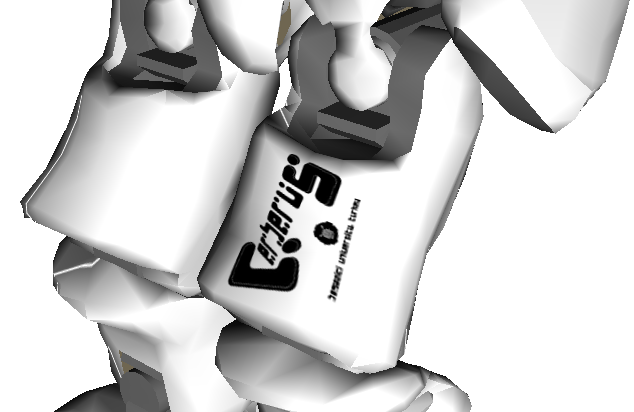
\includegraphics[height=0.35\columnwidth]{figs/naosim_legs_with_logo_closeup.png}
  \end{tabular}}
  \caption{Example Sponsor/Team Logo placement on legs.}
  \label{fig:sponsor}
\end{figure}

\subsection{Communications}

The robots must play without human control. Communication is only allowed among robots on the field and between the robots and the GameController.

\subsubsection{Non-Wireless Communications}
\label{sec:acoustic}
In general there are no restrictions on communication between robots in play on the field using visual signalling (\eg gestures) or the robot's built-in microphones, speakers, and infrared transceivers. However, communication that causes excessive discomfort to an audience, affects the safety of an audience, or violates normal playing rules is not permitted.

\subsubsection{Wireless Communications}
\label{sec:wireless}
The only wireless hardware allowed to be used by the teams are the wireless network cards built into the NAOs, and the access points provided by the event organizers. All other wireless hardware must be deactivated. A team may be disqualified if one of the team members violates this rule.

Each team will get a range of IP addresses that can be used both for their robots and their computers. The network configuration (\eg IP addresses, channels, SSIDs, and required encryption) of the fields will be announced at the competition site.

Wireless robot-to-robot communication among the robot players is allowed, as long as it uses the access points provided by the event organizers (using the so-called ad-hoc mode is prohibited), messages are sent via UDP broadcast, and the SPL standard message packet is used. The SPL standard message packet is specified in the header \emph{SPLStandardMessage.h} that is distributed with the latest GameController release at \url{https://github.com/RoboCup-SPL/GameController}.

Each team will be assigned a range of IP-addresses that can be used for robot-to-robot communication. Each team will also be allocated a single UDP port for network broadcasts. Specifically, a team's port will be 10000 plus that team's GameController number. All robot-to-robot communication during matches must be sent via UDP broadcast. Unicast communication between robots is prohibited.

The amount of data transmitted by a team in a single game is limited. The limit is measured as the total number of UDP packets sent by any robots of a team. A team may not exceed \TeamMessageLimit packets per game. This limit will be lowered in future competitions to encourage smart event-based communication. If a team exceeds their limit the game is scored with 0 goals for the offending team. Robot-to-robot communication that violates the SPL rules result in a game scored with 0 goals for the offending team (even when discovered after the game was finished).

The GameController tracks the number of messages that have already been sent and includes the counters per team in \texttt{RoboCupGameControlData}.

In addition to robot-to-robot communication, robots may send:
\begin{itemize}
 \item Additional status update packages that are sent to the GameController.
 \item Team specific debug information may be sent to an external computer owned by the team. A robot may send debug information at most once every 2 seconds in a single UDP packet.
\end{itemize}
These additional packages do not count towards the team's data limit and may not be used for robot-to-robot communication. They must be sent as unicast and may not be sent as broadcast.

Teams and their robots must not listen into another team's communication.

Robots are not allowed to be connected to access points of fields that are currently running official games of other teams.
Robots may only communicate on fields that are not running an official game or fields which they are playing on.

The GameController will use UDP to connect to the robots. The source distribution of the GameController provides the header file \emph{RoboCupGameControlData.h} that defines all messages sent by the GameController to the robots. They correspond to the \emph{robot states} described in Section~\ref{sec:robot_states}.

Robots send status updates (defined in \emph{RoboCupGameControlData.h}) to the GameController. These return packets must be addressed directly to the GameController PC (\ie not broadcast) and sent on the GameController return UDP port specified by the symbol \verb!GAMECONTROLLER_RETURN_PORT! in \emph{RoboCupGameControlData.h}.

The use of remote processing/sensing is prohibited.

\newpage

\section{Game Process}
\label{sec:game_process}

\subsection{Structure of the Game}
\label{sec:game_struct}

A game consists of three parts, the first half, a half-time break, and the second half. Each half is \qty{10}{\minute} counted from the initial kick-off.
The half-time break is \qty{10}{\minute}, and during this time both teams may change robots, change programs, or do anything else that can be done within the time allotted.

The head referee signals the commencement of each half with a single whistle blow (that is, the Initial kick-off, \cf Section~\ref{sec:initial-kick-off}).
The head referee signals the end of the first half with two short whistle blows, and the end of the second half with two short plus one long whistle blow.
The head referee should make \textit{all} of these whistle sounds from the T-junction of the half-way line.

The teams/robots will change the goal defended during the half-time break.

\subsection{Robot States}
\label{sec:robot_states}

Robots can be in \textit{eight} different \emph{primary} states (see Figure~\ref{fig:robot_states}). Wireless connection must be available, so these states will be set by the GameController. Teams must implement code to receive and correctly respond to wireless GameController packets, and also give a visual indication of the game state.

\textbf{The usage of the button interface as a replacement for any GameController commands/transitions is not allowed in the main competition!}

Should, on both teams, at least two robots have problems with the Wifi/GameController connection the head referee should issue a referee timeout (see Section~\ref{sec:referee_timeout}).
If fewer robots do not respond to the GameController then they are, at the beginning, not included in the game (via a `Request for Pick-up', see Section~\ref{sec:request_for_pickup}), and the game starts without the offending robot.

\begin{description}
  \item [Unstiff.] It helps to facilitate a consistent and safe handling of the robots for remote competition. During any state, if all head buttons are pressed at least one second, the robot should move to a safe seated/crouched position and \textit{unstiffen} all joints. So while in the \textit{unstiff} state the robot is not allowed to move in any fashion! Pressing the chest button once while in the \textit{unstiffen} state, permits the robot to \textit{stiffen} it’s joints and return to the initial state, or a state as indicated by GameController.

  \item[Initial.] After booting, the robots are in their \emph{initial} state. The robots are not allowed to be moving in any fashion besides initially standing up. Shortly pressing the chest button will switch the robot to the \emph{penalized} state.

  \item[Ready.] In this state, the robots walk to their legal positions for Kick-Off  (\cf Section~\ref{sec:kick-off}) or a Penalty Kick (\cf Section~\ref{sec:penalty_free_kick})). They remain in this state, until the head referee decides that there is no significant progress, up to a maximum of \KickOffAutoTime for a Kick-off and \PenaltyFreeKickSetupTime for a Penalty Kick.
  The GameController can activate substates for kick-off and penalty kicks.
  This state is not available if only the button interface is implemented.

  \item[Set.] In this state, the robots stop and wait for Kick-Off  (\cf Section~\ref{sec:kick-off}) or a Penalty Kick (\cf Section~\ref{sec:penalty_free_kick})).
  Illegally positioned robots are penalized and placed on the side of the field.
  Robots are allowed to move their heads or get up if fallen before the game (re)starts but they are not otherwise allowed to move their legs or locomote in any fashion.
  If a robot cannot get up, fallen robot is called~(\cf Section~\ref{sec:fallenrobots}).
  The penalty time counter is frozen during this state.
  Note that all penalised robots are left in place (on the side of the field, or in-place for motion in set) and must wait to get unpenalized.
  The GameController can activate substates for kick-off and penalty kicks.
  This state is not available if only the button interface is implemented.

  \item[Playing.] In the \emph{playing} state, the robots are playing soccer. Shortly pressing the chest button will switch the robot to the \emph{penalized} state. During the \emph{playing} state, the GameController can activate the substates for free kicks (\cf Section~\ref{sec:free_kick}).

  \item[Penalized.] A robot is in this state when it has been penalized. It is not allowed to move in any fashion,  this includes stopping the head turning. Shortly pressing the chest button will switch the robot back to the \emph{playing} state.

  \item[Finished.] This state is reached when a half is finished. The robots then have to sit down.

  \item[Calibration.] This state denotes the robot is acting with automatic calibration. This state may only be entered from \textit{Initial} by first pressing the \textit{front} head button concluded by the chest button, for at least one second by the referees.


\end{description}

\begin{figure}[t]
	\centerline{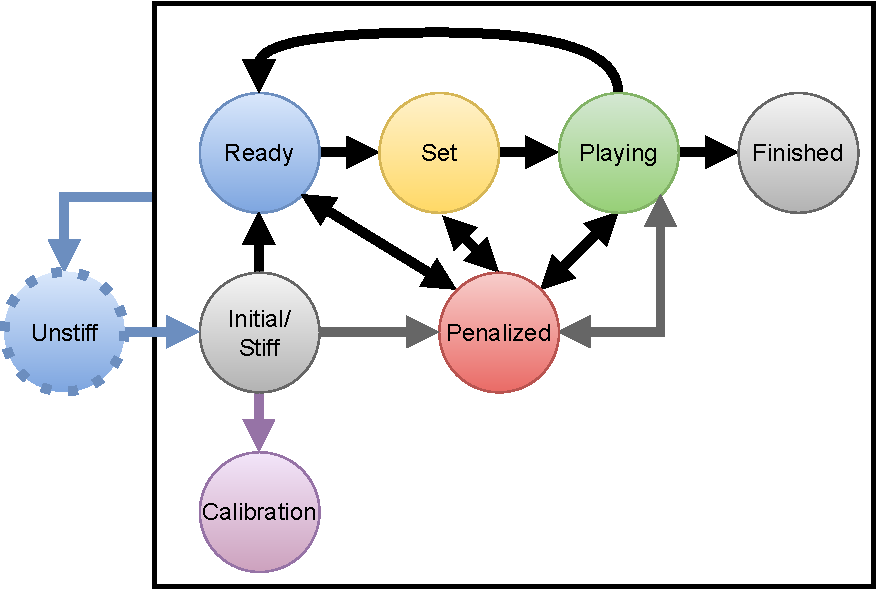
\includegraphics[width=0.9\columnwidth]{figs/states_new.pdf}}
	\caption{Diagram of the robot states.
    \\\textbf{Chest button} transitions are shown as gray arrows. However, any transition possible should be sent by the GameController.
    \\\textbf{GameController} transitions are shown as black arrows.
    \\Calibration transitions are shown as purple arrows which mean pressing the \textbf{front head button + the chest button}.
    \\From any state it can be transitioned to the \textit{unstiff} state, shown as a blue arrow, via pressing all \textbf{three head buttons}. Pressing all \textbf{three head buttons} in the \textit{unstiff} state allows a transition to the initial state, or a state as indicated by the GameController.}
	\label{fig:robot_states}
\end{figure}

The referee will announce the start of the \textit{Playing} state with a single whistle blow.
The GameController Playing signal will be delayed by \PlayingDelayTime.
This delay applies to both kick-off and penalty shots.
Robots that begin moving their legs or move in any fashion during \emph{set} (\ie before the referee blows the whistle) will be penalized \textit{in place} on the field via the ``Motion in Set'' (\cf Section~\ref{sec:motion_in_set}) GameController signal until the GameController transmits the \emph{playing signal}. A robot will be moved back to its original position if it has moved significantly before becoming penalized.
Note that responding to a whistle on another field will result in this penalty.

The current game state should be displayed on the LED in the torso. The colors corresponding to the game states are:

\begin{itemize}
  \item Unstiff: Blue-Blinking
  \item Initial: Off
  \item Ready: Blue
  \item Set: Yellow
  \item Playing: Green
  \item Penalized: Red
  \item Finished: Off
  \item Calibration: Purple
\end{itemize}

The current GameController requires robots to know both their team number and their robot number within the team. It is each team's responsibility to make sure this is correctly configured. It is recommended that the robot indicates its number within the team on boot up so that this can be easily checked at the start of the game.

\subsection{Goal}
\label{sec:goal}
A goal, including own goal, is achieved when the entire ball (not only the center of the ball) goes over the goal-side edge of the goal line, \ie the ball is completely inside the goal area\footnote{The goal line is part of the field.}.

The head referee signals a goal by a single whistle blow, followed by the call ``Goal \textless color\textgreater''.
The head referee should point with one arm towards the center of the field.
To assist robots listening for whistles, the referee should blow the whistle from on the carpet at the end of the fields where the goal was scored.

The GameController signal (to the robots) of a goal being scored, will be delayed by \GoalScoredDelay.

\subsubsection{Invalid Goal}
\label{sec:invalid_goal}

A goal is invalid (that is, it can never be awarded) in the following circumstances:
\begin{enumerate}
    \item When an Indirect Kick has not occurred (see~Section~\ref{sec:indirect_kick}).
    \item When the last contact of the ball was with an attacking robot that played the ball with the arms/hands as defined in Section~\ref{sec:hand_ball}. However, an own goal may be scored by any defending robot playing with arms/hands.
    \item When a team scores on themselves and there are no opponent robots on the field that are active (a definition of \emph{active} is given in Section~\ref{sec:fallenrobots}).
\end{enumerate}

In these cases a goal is not scored (that is, the goal is ruled invalid), and the game will proceed with a Goal Kick (\cf Section~\ref{sec:free_kick}). The head referee should also advice why the goal is invalid, such as by calling ``Not indirect'', ``Played with hands'' or ``No own goal''.

\subsubsection{Indirect Kick}
\label{sec:indirect_kick}

From any restart in play (Kick-off, Kick-in, Free kick) except for Penalty kick, the attacking team may only score a goal via an indirect kick.
%, providing they have at least 3 active robots on the field at the time the restart occurs (or is awarded in the case of a free kick).
A robot may not score a goal from a direct kick, including via deflections.
The ball must be deliberately played-at a second time (by either another robot, or the same robot) before a goal may be scored.
A deliberate play at the ball includes successfully kicking the ball, dribbling the ball (and subsequently leaving possession of the ball), or the goalkeeper playing at the ball with its hands.
If a robot plays the ball to itself, this means that the ball must leave a circular area of at least \qty{0.75}{\metre} the robot before the ball is played a second time and to be considered as an indirect
kick.

\textbf{Example 1:} Player 2 (of the red team) kicks the ball to Player~3, who then kicks the ball into the goal. This is a successful indirect kick, and the goal counts.

\textbf{Example 2:} Player 2 (of the red team), kicks the ball at the goal, and it is deflected of the side of the foot of a blue-team robot into the goal. This is \textit{not} and indirect kick, and the goal does not count.

\textbf{Example 3:} Player 2 (of the red team), kicks the ball ``upfield''. A blue-team robot kicks the ball a short distance, after which Player~2 kicks the ball again into the goal. This is a successful indirect kick, and the goal counts.

\textbf{Example 4:} Player 2 (of the red team), walks up to and dribbles the ball. To be an indirect kick, Player~2 must then stop, and visibly back-away from the ball, before approaching to dribble a \textit{second} time. The robot then scores. This is a successful indirect kick.

Note that an own-goal may always be scored without requiring an indirect kick.

\subsection{Initial Kick-off}
\label{sec:initial-kick-off}

The first kick-off at the start of each half is the initial kick-off.
Before the initial kick-off, \ie before the start of each half, all robots must be in the \textit{unstiff} state and must be placed on the sidelines in their own half of the field, by the referees according to Figure~\ref{fig:initial_positions}.
Once the robots receive the \emph{ready} signal from the GameController, they are to proceed as described in Section~\ref{sec:kick-off}.

\begin{figure}[t!]
	\begin{center}
		\leavevmode
		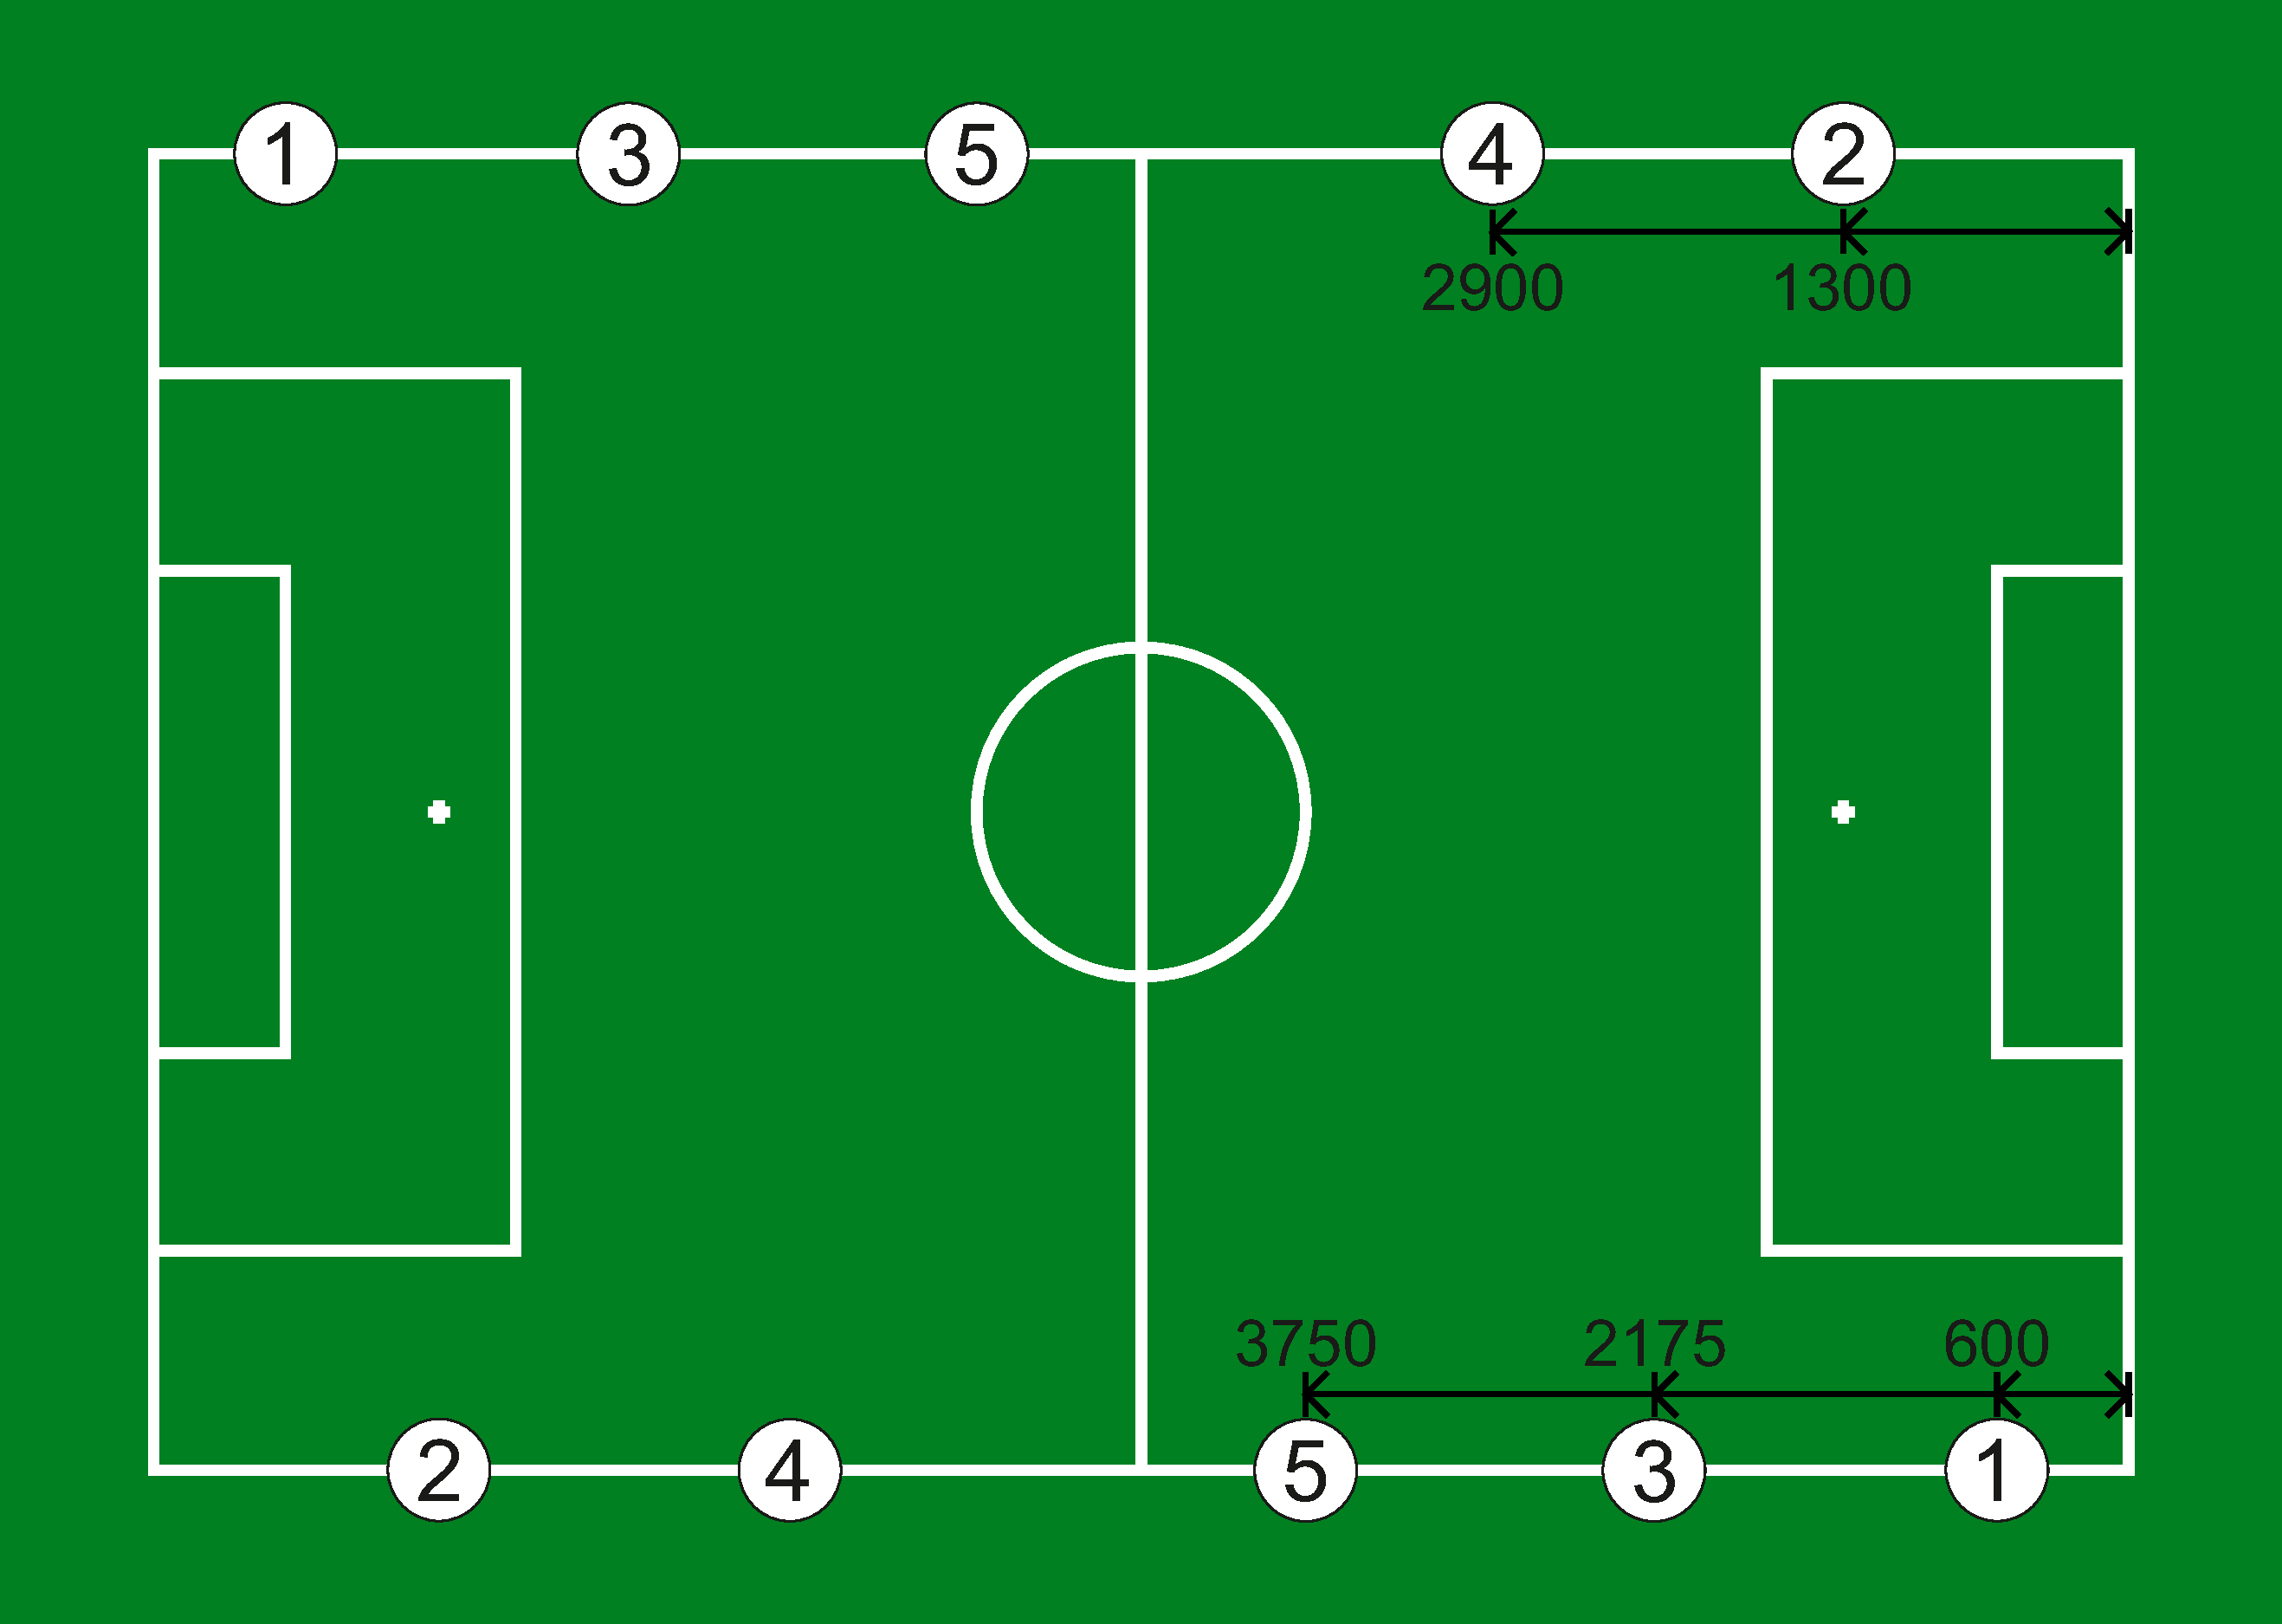
\includegraphics[width=1\columnwidth]{figs/initial_positions.pdf}
		\caption{Positions, player numbers and distances from the center of the goal line for the initial kick-off of the robots.}
		\label{fig:initial_positions}
	\end{center}
\end{figure}

\subsection{Kick-off}
\label{sec:kick-off}
For kick-off, the robots listening to the wireless GameController run through three states: \emph{ready}, \emph{set}, and \emph{playing}.
It is to a team’s responsibility to have their robots listening to the GameController!

In the ready state, the robots should walk to their legal kick-off positions.
The attacking team can be positioned anywhere within their own half.
The defending team can be positioned within their own half, except for inside the center circle including its line.
No player is allowed to touch the halfway line.
Both teams are also subject to restrictions on the penalty box~(\cf Section~\ref{sec:illegal_positioning}).
The green carpet border, except for the area of the goal, is not part of either teams own half. All robots that do not reach legal positions will be penalized with the ``Illegal Position'' penalty~(\cf Section~\ref{sec:illegal_positioning}).


In the \emph{Set} state, the robots must not move~(\cf Section~\ref{sec:robot_states}). A referee places the ball on the center point of the center circle. If the ball is moved by one of the robots during \textit{Set} it is moved back by one of the referees.

There is no manual placement of any robot.

The head referee signals the kick-off by a single whistle blow, followed by the call ``Playing''. The head referee must signal this from the T-junction of the half-way line.

After the head referee has signalled the kick-off, the robot's state is switched to \emph{playing} by the GameController.
The defensive team must stay outside of the center circle until the ball is in play.  The ball is in play once it is touched by the attacking team or once \emph{\KickOffBallFreeTime} have elapsed in the playing state.
The GameController and head referee will indicate this by the call `` Ball Free''.
If a defensive player enters the center circle before the ball is in play, the ``Illegal Position'' penalty is applied (\cf Section~\ref{sec:illegal_positioning}).

Note a goal may not be scored from within the center circle on kick-off~(\cf Section~\ref{sec:invalid_goal}), and that indirect kick rules apply~(\cf Section~\ref{sec:indirect_kick}).

\subsection{Kick-in}
\label{sec:kick_in}

A ball is considered to have left the field when there is no part of the ball over the outside of the boundary line (\ie the line itself is in). If the ball leaves the field it will be replaced on the field by an assistant referee. Balls are deemed to be out based on the team that last touched the ball, irrespective of who actually kicked the ball.

If the ball goes over a sideline then the assistant referee will replace the ball back on the point of that sideline where it went out. A free kick (\cf Section~\ref{sec:free_kick}) is awarded to the team that did \emph{not} last touch the ball by the referee calling ``Kick-in \textless color\textgreater''.

If the ball goes over an end-line then the assistant referee will replace the ball back on the field, depending on which team last touched the ball.

\begin{itemize}
  \item If the ball was last touched by the defensive team, a \emph{Corner Kick} (\cf Section~\ref{sec:free_kick}) is awarded to the attacking team. The referee calls ``Corner Kick \textless color\textgreater'' and the ball is placed on the corner on the same side of the field that the ball was kicked-out.
  \item If the ball was last touched by the offensive team, a \emph{Goal Kick} (\cf Section~\ref{sec:free_kick}) is awarded to the defensive team. The referee calls ``Goal Kick \textless color\textgreater'', and the ball is placed on the corner of the Goalbox on the same side of the field that the ball was kicked-out. That is, the corner inside the field, not the t-junction where the goalbox meets the goal line.
\end{itemize}

In these examples, ``red half of the field'' refers to the half the red team is defending.

  \textbf{Example 1:} The red goal keeper kicks the ball out the end of the field to the right of the goal. The referee calls ``Corner Kick blue'', the ball is placed on the corner to the right of the goal and a free kick is started.

  \textbf{Example 2:} A blue robot kicks the ball out the end of the field to the right of the goal the red team is defending. The referee calls ``Goal Kick red'' and the ball is placed on the right corner of the goalbox.

  \textbf{Example 3:} A blue robot at midfield kicks the ball over the left sideline \qty{2}{\metre} into the red half of the field. The referee calls ``Kick-in red'' and the ball is replaced on the left sideline where it went out.

  \textbf{Example 4:} A blue robot kicks the ball but the ball touches a red robot at midfield before leaving the field near the center line. The ball is regarded as out by red, the referee calls ``Kick-in blue'' and the ball is replaced on the kick-in line where it went out.

\subsection{Free Kick}
\label{sec:free_kick}

A Free Kick is initiated:
\begin{itemize}
  \item When the ball goes over the sidelines, termed \emph{Kick-in}.
  \item When the ball goes over the end-lines initiated by the defensive team, termed \emph{Corner Kick}.
  \item In place of an end-line Kick-in initiated by the offensive team, also termed a \emph{Goal Kick}.
  \item A pushing penalty (see Section~\ref{sec:player_pushing}) awarded near the ball, termed a \emph{Pushing Free Kick}.
  \item A pushing penalty (see Section~\ref{sec:player_pushing}) awarded against the defending team within their own penalty box, termed a \textit{Penalty Kick}.
\end{itemize}

The head referee will announce a Free Kick, calling one of:
\begin{enumerate}
  \item For a \textit{Pushing Free Kick}: ``Foul \textless color\textgreater \textless number\textgreater'' for the pushing robot.
  \item For a \textit{Penalty Kick}: ``Foul \textless color\textgreater \textless number\textgreater'' for the pushing robot, followed by ``Penalty Kick \textless team\textgreater''.
  \item For all other free kicks: ``Kick-in/Goal Kick/Corner Kick \textless team\textgreater'' for the team that did not last touch the ball.
\end{enumerate}

The GameController will then activate the substate for the respective free kick. Note that in the case of the Pushing Free Kick the substate is activated automatically through the ``Foul''.
The team who is awarded the Free Kick (termed the attacking team) has \qty{\FreeKickTime}{\second} to complete the kick.
For a ``Penalty Kick'', the game instead proceeds as described in Section~\ref{sec:penalty_free_kick}.

When necessary, the referee may need to place the ball.
For a Pushing Free Kick, the ball will be left in place, and only repositioned in accordance with the pushing rules (see Section~\ref{sec:player_pushing}).
If the ball left the field, the ball will be positioned as described in Section~\ref{sec:kick_in}.

During the Free Kick, only the attacking team may approach within \FreeKickRadius to the ball, with the exception of the defensive goalkeeper. All other robots of the defensive team must move away from the ball. The defensive goalkeeper may be within the \FreeKickRadius radius, provided that it is within the Penalty Box and does not touch the ball. Defensive robots that violate these restrictions are penalised with the ``Illegal Positioning'' penalty (see Section~\ref{sec:illegal_positioning}) which results in a standard removal penalty~(see Section~\ref{sec:removal_penalty}).
Additional penalties against any further robots during the free kick, including Pushing, do not result in an additional Free Kick, but still use the appropriate removal penalty.

A Free Kick is deemed completed and play returns to normal if:
\begin{itemize}
    \item The attacking team touches the ball, except for a robot getting up which is exempt from this rule.
    \item The \qty{\FreeKickTime}{\second} time period expires (or the game time expires).
\end{itemize}
The head referee will announce a Free Kick is completed, by ``Ball Free'', and the GameController resumes the game state \emph{playing}. Note that the substate will be automatically left after the \qty{\FreeKickTime}{\second} time period expires.

\subsubsection{Penalty Kick Procedure}
\label{sec:penalty_free_kick}

When the GameController activates the Penalty Kick, the game changes to the \textit{Ready} state.
This denotes that the robot's are given time to setup and prepare for the penalty kick.
Similar to kick-off, the game clock is \textit{paused} during finals games only.
The referees should pick up the ball.

Robots have \qty{\PenaltyFreeKickSetupTime}{\second} to get into position for the Penalty Kick. At the end of \qty{\PenaltyFreeKickSetupTime}{\second}, the game changes to the \textit{Set} state.
Similar to a kick-off, during the Set state the robots are waiting for the Penalty Kick to commence.
Standard penalties apply.
Additionally, only the goalkeeper robot from the defending team may be within the penalty box. The goalkeeper robot must also be touching the goal line.
Only one robot from the attacking team may be within the penalty box, and it may not block the penalty spot.
Blocking the penalty spot is considered to be an illegal position.
All robots that do not reach legal positions will be penalized with the ``Illegal Positioning'' penalty~(\cf Section~\ref{sec:illegal_positioning}).

The referee should also place the ball on the penalty spot during \textit{Set}.
The referee signals the Penalty Kick commences by blowing the whistle once, and calling ``Playing''.
The game switches to the \textit{free kick} sub-state of the \textit{Playing} game state, and the game clock is resumed.
(Note that the GameContoller signal is delayed by \qty{\PlayingDelayTime}{\second} when switching from \textit{Set} to \textit{free kick} sub-state).
The attacking team has \qty{\PenaltyFreeKickTime}{\second} to complete the Penalty Kick.

During the Penalty Kick:
\begin{enumerate}
    \item The defensive goalkeeper robot must always be in contact with the goal line, and must remain on its feet. The goalkeeper is only permitted to ``dive'', and be off it's feet after the attacking robot has touched the ball.
    \item The attacking robot may move freely.
    \item All robots must be within the field-of-play. That is, robots may not be outside the field lines, but within the field border.
    \item No other robots may enter the penalty box (\cf Section~\ref{sec:illegal_positioning}).
    \item Additional penalties against any further robots, including Pushing, do not result in an additional Free
    Kick, but still use the appropriate removal penalty.
\end{enumerate}

The attacking robot (taking the penalty kick) may only score a goal if it touches the ball once.
Once the attacking robot has touched the ball, it may not score a goal until another robot (from either team) touches the ball.
If this robot ``scores'', it results in a Goal kick~(\cf Section~\ref{sec:invalid_goal}).

The Penalty Kick is deemed completed if:
\begin{itemize}
\item The attacking team touches the ball, even if the robot has fallen.
\item The \qty{\PenaltyFreeKickTime}{\second} time period expires (or the game time expires).
\end{itemize}

The head referee will announce a Free Kick is completed, by ``Ball Free'', and the GameController
resumes the game state \emph{playing}. Note that the substate will be automatically left (returning to the \textit{playing} state) after the \qty{\PenaltyFreeKickTime}{\second} time period expires.

Note that the restrictions on the attacking robot still apply after the penalty kick is complete.

\subsection{Game Stuck}
\label{sec:game_stuck}

In the event of no substantial change in the game state for \qty{\GameStuckTime}{\second}, this is considered a game stuck.  ``Substantial change'' can consist of a robot seeing and moving towards the ball OR robots exploring the field (presumably in an attempt to find the ball).

The main referee has two options how to solve the game stuck and to reestablish the chance of progress in the game. The intention of the game stuck rule is to achieve progress with as little intervention as possible, \ie the \emph{Local Game Stuck} rule will be preferred, but only if there is a chance that its application will result in progress in the game.

\subsubsection{Local Game Stuck}
\label{sec:game_stuck:local}

If one robot is preventing the game from proceeding --- perhaps by circling the ball repeatedly without kicking the ball --- it is recommended to improve progress by removing this one robot.
The head referee calls ``Local Game Stuck \textless robot\textgreater'' for this robot, which is penalized (\cf Section~\ref{sec:pen_local_game_stuck}).

\subsubsection{Global Game Stuck}
\label{sec:game_stuck:global}

If no robots have made progress towards the ball or began to explore the field in \qty{\GameStuckTime}{\second} Global Game Stuck should be called be called on the team whose robot is \textit{not} nearest the ball.
The referee calls ``Global Game Stuck \textless color\textgreater''.

Once the referee calls Global Game Stuck, players enter the Ready state, and a new kick-off is awarded to the team that was closer to the ball when the Global Game Stuck was called. A global game stuck can only be called if at least one robot has touched the ball since the previous kick-off.

\subsection{Request for Pick-up}
\label{sec:request_for_pickup}

Either team may request that one of their players be picked up (called ``Request for Pick-up'').
In the Playing or Ready state, players may only be picked up for hardware failures.
In all other states, players may be picked up for any reason.

Every change (hardware or software) is allowed during a request for pick-up. In particular,
it is permitted to change batteries, fix mechanical problems, reboot the robots, and change configuration files.
It is also allowed to replace a broken robot by a substitute robot.
It is discouraged to change the robot's control program, \textbf{but not forbidden}.

Any strategic ``Request for Pick-up'' is not allowed.
That is, gaining an advantage by removing the robot from the game.
In this case, the head referee will indicate when the robot is no longer affecting play and can be removed from the field by an assistant referee.

To prevent mistakes and confusion during games, only team leaders should make a ``Request for Pick-up'', and only one designated person per team shall accept the robot from the referee, and hand it back after fixing the problem.
The returning robot may be returned following the normal replacement procedure once at least \qty{\StandardPenaltyTime}{\second} have elapsed since the robot was removed from play.
Note that this penalty does not follow the standard removal procedure, and hence does not count towards the incremental penalty count.
If the picked-up robot was penalized, the penalty time of the robot counts down with the game clock throughout the pick-up.

The robot should be returned to the assistant referees in the \emph{penalized} state.
Note here, that the returning robot or the substitute robot will have to wait out any remaining penalty time of the picked up robot after the team handed their robot back to the assistant referees.

\subsection{Request for Timeout}
\label{sec:request_for_timeout}

Each team can call a \textbf{maximum of 1 timeout per game} with a total time of no more than \textbf{5 minutes}. During this time, both teams may change robots, change programs, or anything else that can be done within the time allotted.  During normal game time, a team may call a timeout at any stoppage of play (after a goal, stuck game, before a half, etc.). Alternatively, a team may call a timeout before a penalty shootout if they have not used their timeout yet (\cf Section~\ref{sec:penalty_shoot-out}).

The timeout ends when the team that called the timeout says they are finished, at which time they must be ready to play. The other team must be ready to play at the time the timeout runs out, or \textbf{2 minutes} after a prematurely called end of the timeout, whichever is earlier. If the other team is not ready to play in time, it has to call a timeout of its own.

The clock stops during timeouts, even during the preliminaries, and is reset to the time when the current stoppage of play began.

After the completion of the timeout, the game resumes with a kick off for the team which did not call the timeout.

If a team is not ready to play at the assigned time for a game, the referee will call the timeout for that team. After the expiration of such a timeout, if the team is still not ready to play then the referee shall start the game with only one team on the field.  The team that was not ready can return its robots to the field as per the rules for ``Request for Pick-up''. If both teams are not ready, the referee will call timeouts for both teams. This ``double timeout'' expires after 10 minutes.

\subsection{Referee Timeout}
\label{sec:referee_timeout}
The head official may call a timeout at any stoppage of play if he or she deems it necessary.  A referee timeout should only be called in dire circumstances --- one example might be when the power to the wireless router is down or no robot listens to the GameController.  However, when and whether to call a referee timeout is left up to the head referee.

Referees may call multiple timeouts during a game if needed.  Teams may do anything during these timeouts, but they must be ready to play \textbf{2 minutes} after the referee ends a timeout.  The referee should end the timeout once he or she believes the circumstance for which the timeout was called has been resolved.  In cases where the circumstance for which the timeout was called is not resolved within 10 minutes, the chair of the technical committee should be consulted regarding when/if play should continue.

The team who would have kicked off if the timeout had not been called shall kickoff when the game resumes.

\subsection{Extra Time}
\label{sec:extra_time}
The head official may decide to add time to the clock if a substantial delay (such as an enormous wireless delay) causes excessive game time to be lost.  The decision to add time to the clock should be made immediately after the incident.  The person working the GameController should execute this addition of time using the GameController interface.

\subsection{Mercy Rule}
\label{sec:mercy_rule}
A game will conclude once the game score shows a goal difference of 10.  Ending the game is mandatory once a goal difference of 10 is reached.

\subsection{Rules for Forfeiting}
\label{sec:forfeit}

Teams who do not make a good faith effort to participate in a scheduled game are considered to forfeit the game.

If a team notifies the technical committee that they wish to forfeit less than two hours before their scheduled game time, simply fails to show up for their game, or decides during their game that they wish to forfeit, then the opposing team will play the match against an empty field.  However, any own goals will not be scored.  Hence, after an opponent forfeits, the team playing against an empty field cannot do worse than they were doing at the time the opponent decided to forfeit.  Teams may choose to forfeit at any stoppage of play.  However, once a forfeit is announced, they may not reverse this decision.

If a team notifies the technical committee that they wish to forfeit at least two hours before their schedule game time, the following procedure will be followed.

\begin{itemize}
  \item If a team chooses to forfeit a match in the round robin games the other team plays the match against an empty field.  However, any own goals will not be scored.
  \item If a team chooses to forfeit in a knock-out game it gets replaced by the next best qualified team, \ie the team it kicked out or left behind in the round robins.
\end{itemize}

Note that there are a few unlikely cases that are not covered by these rules.  If a situation is not covered by these rules, the technical committee and the organizing committee will work together to make a decision.

Any forfeit will result in a qualification penalty being recorded (\cf Section~\ref{sec:qualificationPenalties}) but the circumstances of the forfeit will affect the severity of the offence and the impact on future qualification.

\subsection{Penalty Kick Shoot-out}
\label{sec:penalty_shoot-out}

A penalty kick shoot-out is used to determine the outcome of a tied game when an outcome is required (for example, when team progression is tied on all tie-break factors, during the promotion round, intermediate round, quarter finals, semi finals, third place or final).
There will be a no break between the end of the game and the start of the penalty kicks. As well as no change of robot's code is allowed!

All penalty shots are taken against the same goal\footnote{Which goal to take for the shoot-out is decided by in accordance with the teams, or otherwise by a coin toss.}.
At all stages of the competition, the penalty kick shoot-out will consist of three penalty kicks per team.
The first (left) team in the GameController will have the striker robot for the first penalty kick.
A team that has scored the most goals at the conclusion of these will be declared the winner. A winner can also be declared before the conclusion of the penalty shoot-out if a team can no longer win. If the two teams remain tied after three penalty kicks, then a sudden death shoot-out will follow until a definite winner is found.

No timeouts may be called during the penalty shootout. However, a team may request a timeout before the penalty shootout starts if they have a timeout remaining for this game. \todo{No change of code allowed?}

Before the penalty shootout begins, each team must hand over to referees up to 6 prepared robots that may participate in the penalty shootout. No robots may be added once the penalty shootout starts. Robots that will not participate in the shootout must not be on the wifi network and must stay outside of the field. All participating robots must be wearing the correct jersey for their player (1-6) and no duplicate numbers are permitted. Before each penalty kick, both teams must select the robot to participate (as goal keeper or striker) in the penalty kick. The team leader communicates the selection to the head referee by privately handing the referee a card with their chosen number. After both teams have selected their player, the GameController operator selects the requested striker and goalie robots from the opposing teams and the GameController communicates that all non-selected robots are substitutes and should remain inactive.

\subsubsection{Penalty Kick}
\label{sec:penalty_kick}

A penalty kick is carried out with one striker robot and one opposing goalkeeper.
The penalty kick commences with the \textit{set} game state activated.
The striker (attacking) robot will be indicated by the GameController, by a suitable flag.

Referees place the ball, the striker, and goalkeeper robots. The ball is placed on the penalty spot closest to the goal being defended. The striker robot is positioned on the edge of the penalty box, facing the ball and the goal. (This striker position is denoted by a small dot made with a felt-tip pen.) The goal keeper is placed with its feet on the goal line and in the center of the goal.
Neither robot is permitted to locomote (move their legs) during the \textit{set} state. Movement of the robot's head and arms is allowed.

If a robot is not responding to GameController it must be in the \emph{penalized} state when waiting for the penalty kick to start.
The referees will use the button interface to switch the robot between playing and penalized.
Only the referees may operate the button interface and no non-standard or extra button sequences are permitted.

The head referee commences the penalty kick by blowing the whistle \textit{once}, and calling ``Playing''.
The GameController activates the penalty kick, switching to the \emph{playing} game state.
Note, the playing signal is delayed~(\cf Section~\ref{sec:robot_states}).

The striker robot is only allowed to contact the ball once.
The time limit for the striker is \PenaltyKickTime after the penalty kick starts.
A penalty shot is over when the ball has come to a full stop after the first contact by the striker robot.
A goal is awarded to the attacking team if a goal has been scored (\ie the ball has completely crossed the goal line).
Otherwise, the score is unchanged.

The goalkeeper robot must always be in contact with the goal line, is not permitted to leave the goal box, and must remain on its feet until the striker robot touches the ball.
The goalkeeper is only permitted to ``dive'', and be off it's feet after the attacking robot has touched the ball.
Furthermore, the goal keeper is not allowed to touch a ball that is completely outside the penalty area (the line is part of the penalty area).
If the goalkeeper violates these rules, then a goal will be awarded to the attacking team.

All rules such as ``Ball Holding'', ``Pushing'' and others are applied during the penalty kick.
A goalkeeper will not be penalized for inactivity during a penalty kick, provided its stiffness is on.
Other penalties are applied as usual.

\subsubsection{Sudden Death Shoot-Out}
\label{sec:sudden_death_shoot_out}

Teams take one additional penalty kick each, and the game decision will be made as follows:

\begin{enumerate}
  \item If only one team scores a goal, that team wins.
  \item If both teams score a goal, the sudden death shoot-out is repeated.
  \item If neither team score a goal, then a shot blocked by the goalkeeper beats a shot blocked by the goalpost which beats a wide shot. For example, if the shot of one team gets stopped by the goalkeeper and the other executes a wide shot, the first team wins. If both shots are wide, the shoot-out is repeated.
  \item If after 3 sudden death penalty shots there is still no winner, the referee will toss a coin to decide the game.
\end{enumerate}

\newpage

\section{Forbidden Actions and Penalties}
\label{sec:forbidden_act}

The following actions are forbidden. In general, when a penalty applies, the robot shall be replaced, not the ball.

\subsection{Penalty Procedure}
\label{sec:penalty_procedure}

When a robot commits a foul, the head referee shall call out the infraction committed, the primary jersey color of the robot, and the jersey number of the robot. The penalty for the infraction will be applied immediately by an assistant referee. The assistant referees should perform the actual movement of the robots for the penalty so that the head referee can continue focusing on the game. The operator of the GameController will send the appropriate signal to the robots indicating the infraction committed.

For penalties that are timed, the penalty time is considered to be over at the end of each half.

\subsection{Standard Removal Penalty}
\label{sec:removal_penalty}

Unless otherwise stated, all infractions result in the removal of the infringing robot from the field of play for a particular amount of time, after which it will be returned to the field of play. This process is called the \textit{standard removal penalty}.

When the head referee indicates a foul has been committed that results in the standard removal penalty, the assistant referee closest to the robot will remove the robot immediately from the field of play. The robot should be removed in such a way as to minimize the movement of the other robots and the ball. If the ball is inadvertently moved when removing the robot, the ball should be replaced to the position it was in when the robot was removed.

The GameController will send the appropriate penalty signal to the robot indicating the infraction committed. If the wireless is not working and the penalty is timed, the assistant referee handling the robot will reset the robot into the \emph{penalized} state for the duration of the penalty. After a penalty is signalled to the robot, it is not allowed to move in any fashion. The removed robot will be placed outside of the field facing away from the field of play.

The initial duration of the standard removal penalty time is \qty{\StandardPenaltyTime}{\second}.
Unless otherwise specified, the penalty time increases by \StandardPenaltyIncrease each time a team commits any infraction.
That is, the first infraction will result in a penalty time of 45 seconds, the second infraction (of any type) results in a penalty time of 55 seconds, the third infraction is 65 seconds, etc.

During the \emph{set} state the penalty time counter will not decrease.

The GameController will keep track of the time of the penalty. The operator of the GameController will signal the assistant referees when the penalty is 10 seconds from being over, so that one of them can place the robot in the half of the field which this robot's team is defending on the sideline that is farther from the ball. The robot should be placed close to the position where the penalty point projects on the sideline. This is illustrated in Figure~\ref{fig:penalty_re-entry_points}.

If there is another robot already in this position, the robot should be replaced at a nearby location along the sideline. When finding a nearby location, locations away from the ball should be preferred, but they \textbf{must} still be in the robot's own half, so that the symmetry of the field can be resolved by the robot's localization system.

With approximately 5 seconds left before the penalty ends, the robot should be turned to face towards the opposite sideline.

\begin{figure}[t]
\centerline{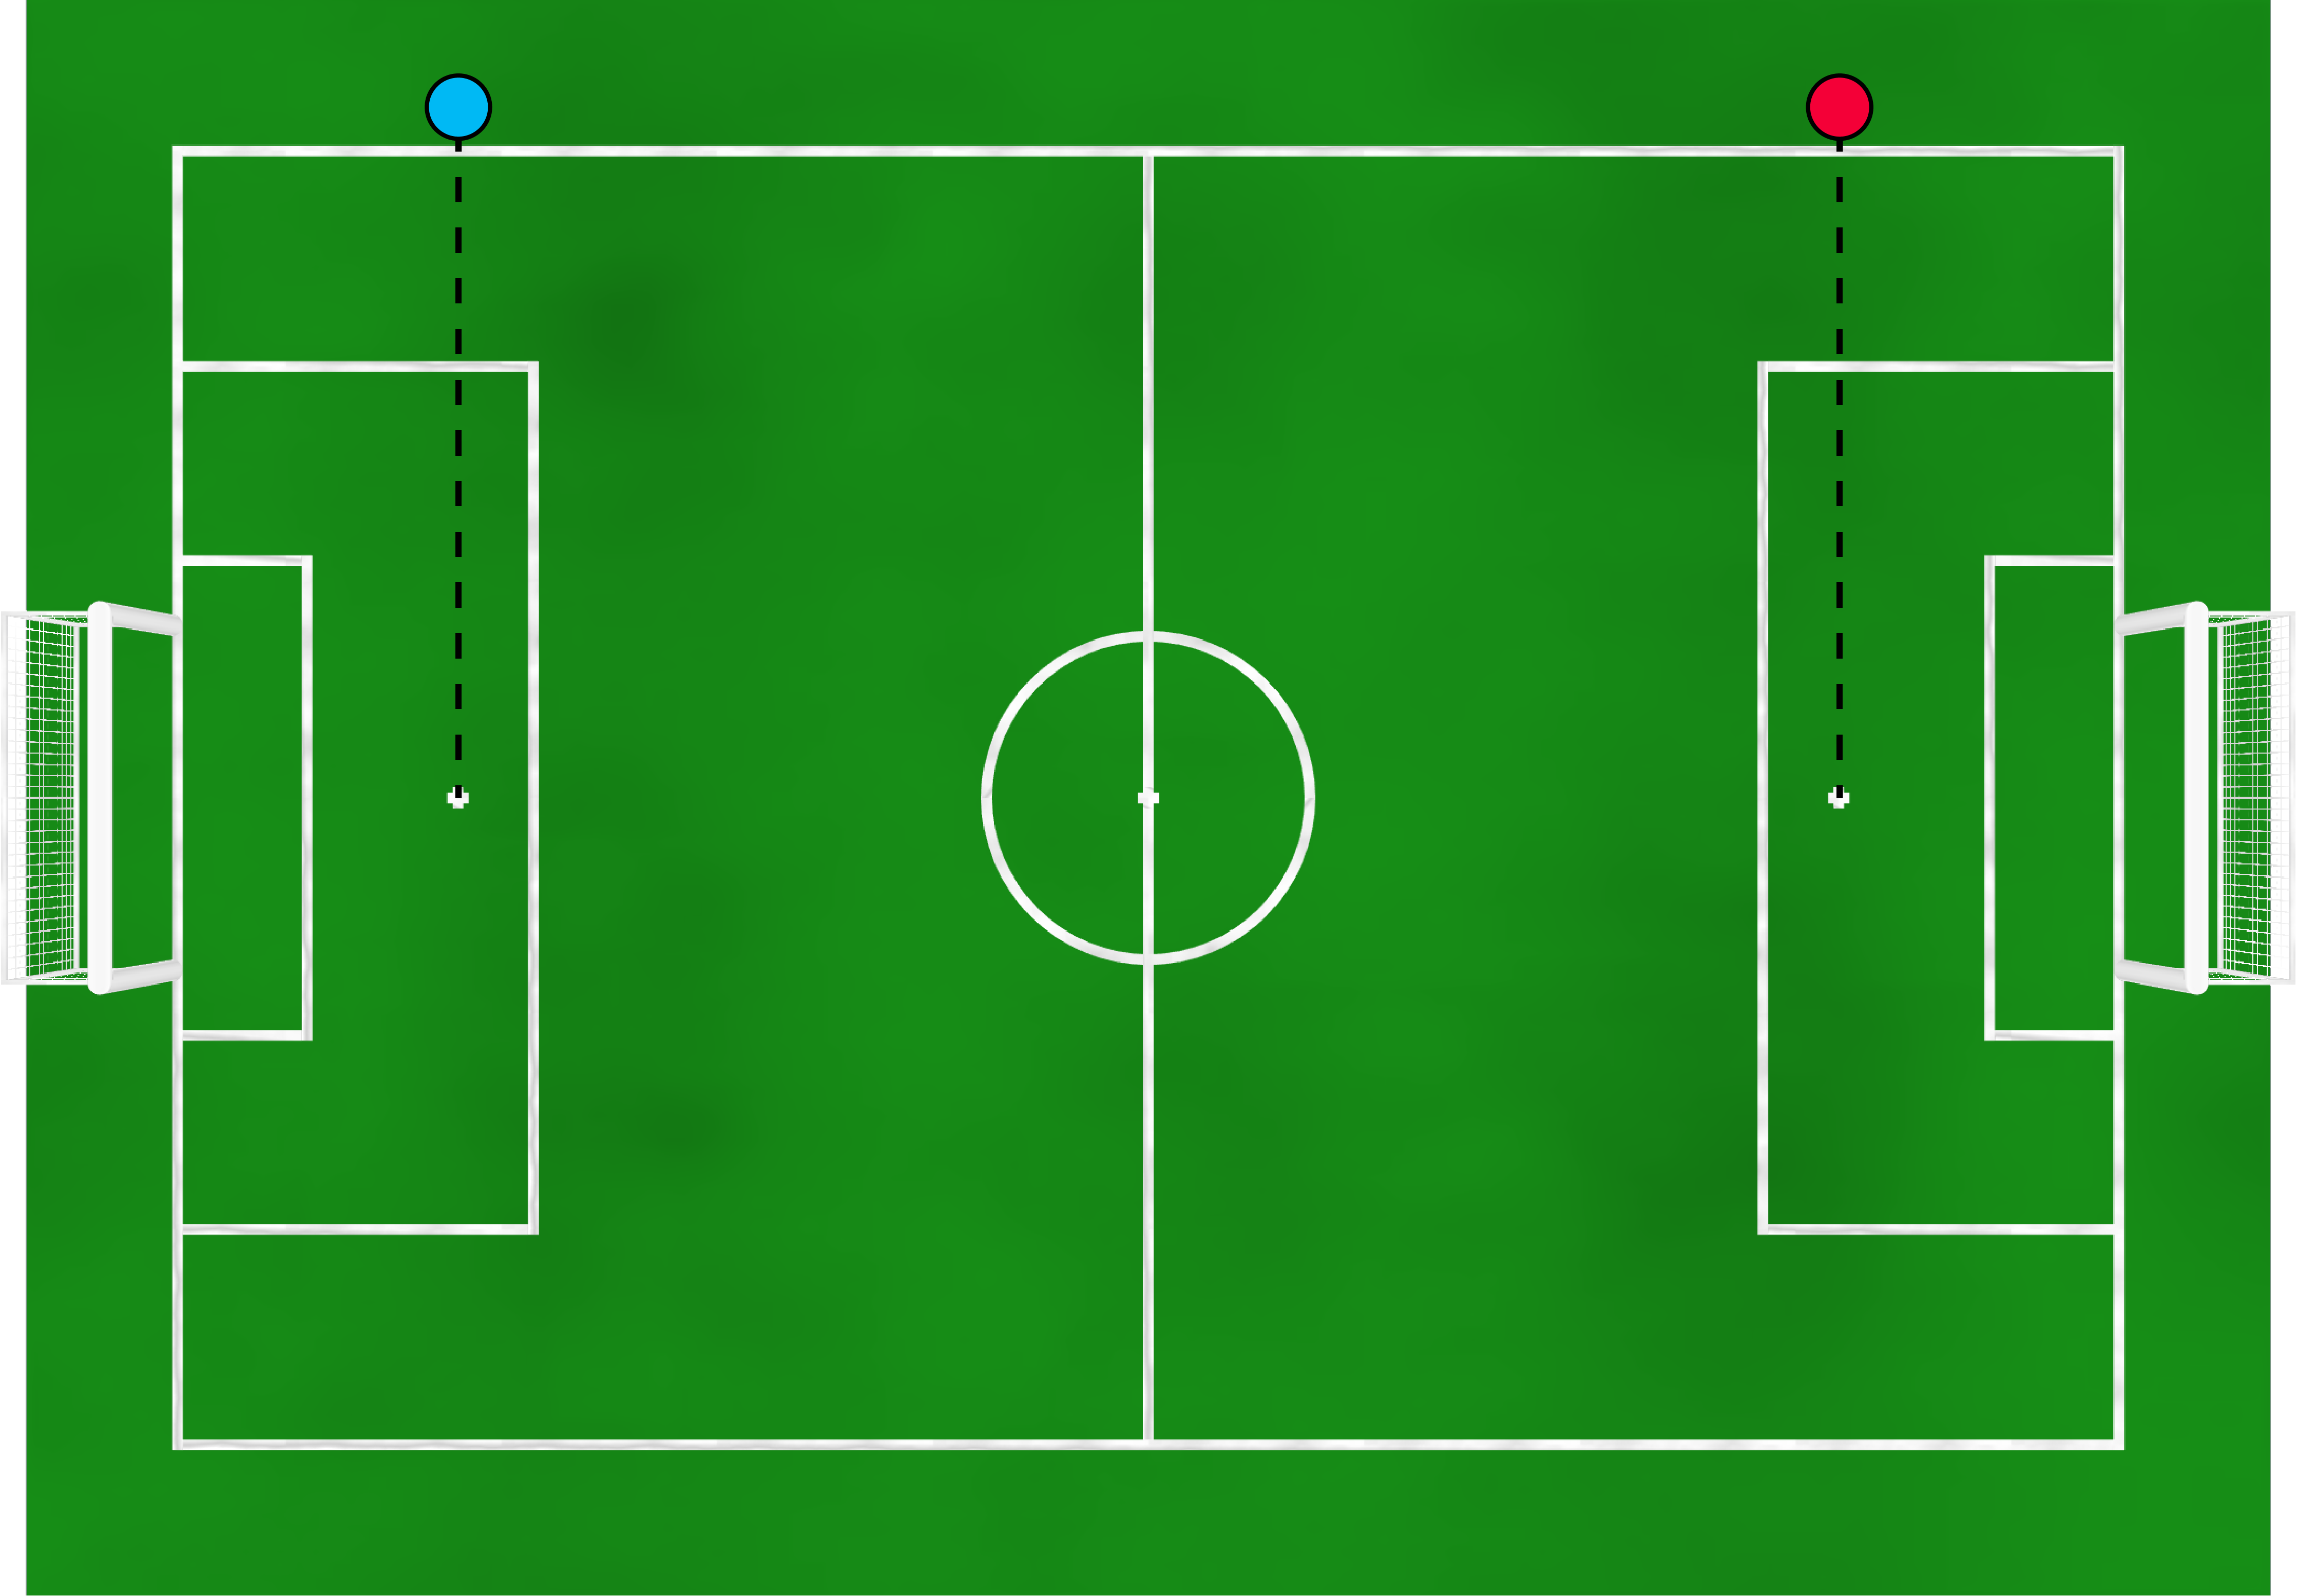
\includegraphics[width=\columnwidth]{figs/penalty_re-entry_points_2020.png}}
\caption{For robots coming back from a standard removal penalty, re-entry points  are inline with the penalty spot in their own half, on the sideline on the side away from the ball.}
\label{fig:penalty_re-entry_points}
\end{figure}

When the robot is on the field again, the operator of the GameController will send the \emph{playing} signal to it. If the wireless is not working, the assistant referee who placed the robot back on the field has to bring it into the \emph{playing} state again.


\subsection{Forbidden Actions}

The following actions are forbidden, but not treated as penalties.
Each forbidden action specifies the actions to be taken by the referees.

\subsubsection{Manual Interaction by Team Members}

Manual interaction with the robots, either directly or via some communications mechanism, is not permitted.
Team members can only touch one of their robots when an assistant referee hands it over to them after a ``Request for Pick-up''.

\subsubsection{Locomotion Type}
\label{sec:locomotion_type}

Robots should clearly demonstrate bipedal walking similar to human walking. Other types of locomotion involving other parts than feet (crawling etc.) are strictly forbidden.
The head referee decides whether a robot's locomotion is appropriate. Robots using inappropriate locomotion types will be removed via ``Request for Pick-up'' until they are able to show appropriate locomotion.

\subsubsection{Damage to the Field}
\label{sec:damage}

A robot that damages the field, or poses a threat to spectator safety, will be removed from the field for the remainder of the game.
%Similarly, a robot that poses a threat to spectator safety will also be removed from the field for the remainder of the game.

\subsection{Illegal Positioning}
\label{sec:illegal_positioning}

A robot penalised under illegal position has the ``Illegal Position'' penalty applied. Illegally positioned robots are subject to the standard removal penalty (\cf Section~\ref{sec:removal_penalty}).
The head referee will call ``Illegal Position  \textless robot\textgreater''\footnote{Referees may interchange ``Illegal Position'' with ``Illegal Defender'' or ``Illegal Attacker'' to help with clarity.}.
Illegal positions are descried below.

For simplicity, Illegal Positioning penalties during the \textit{Set} state (for kick-off or a penalty kick) do not count towards the incremental penalty count\footnote{Historically, the Illegal Positioning penalty only occurred during a kick-off, and other illegal actions were termed Illegal Defender. Illegal Positioning \& Defender have been merged, but the penalty count left unchanged.}.

Refer to Section~\ref{sec:inside_outside} for the definition of \textit{inside/outside} of a region of the field.

\subsubsection{Position for Kick-off}
If a robot is not inside its own half at the time the Set state starts, it will be penalized and removed for 15 seconds. The center line does not count as part of the own half for this penalty, although the area inside the goal does.

\subsubsection{Penalty Box, at all times}

Only \textit{three} players from the \textit{same} team can be the \textit{same} penalty area at the same time\footnote{This means that if no goalkeeper is present, three field players may enter the penalty area to defend the goal.}. This means a total of 6 robots may in the same penalty box at the same time.
\emph{This applies to all game states.}

A robot is within the penalty area if any part of its body is touching the ground inside the penalty box or touching one of its lines.  The penalty is applied when any additional players (whether field player or goalkeeper) enter the area. Note that if a player is pushed into the penalty area by an opponent, this robot will not be subject to removal, unless it fails to exit the area within 5 seconds (or 5 seconds of getting up if the pushing led to falling).

If an illegal defender kicks an own goal, the goal is scored for the opponent. If there is any doubt about whether a goal should count (\eg the illegal defender infraction is called, but the robot scores the own goal immediately afterwards, before it is removed) then the decision shall be against the infringing robot.

\subsubsection{Center Circle, during Kick-off}

The penalty is applied to defensive players that enter the center circle after a kick-off before the ball is in play (\cf Section~\ref{sec:kick-off}).

\subsubsection{Defender Encroachment, during Free-kick}

If a robot of the offending team does enter or not attempt to leave the \FreeKickRadius area around the ball after a Free Kick (\cf Section~\ref{sec:free_kick}) was called, ``Illegal Position'' is called. This rule does not apply for the goalkeeper robot within its own penalty area. Note that the referee should not look for exact distances and rather penalize only those robots who clearly violate this rule. As a guideline, the robots of the offending team should clear the ball within 10 seconds.

\subsubsection{Penalty Box, during Free-kick}

If a robot that enters the relevant penalty box during a penalty kick, except for the goalkeeper (defending team) and one robot of the attacking team, ``Illegal Position'' is called.

\subsection{Motion in Set}
\label{sec:motion_in_set}

Robots may not exit the Set state until either the referee's whistle is detected or a GameController Playing signal has been received.
The head referee will call ``Motion in Set \textless robot\textgreater''.
The offending robot is penalized \textit{in-place} on the field.  They will then be unable to move until they receive the GameController Playing signal.  Motion in Set penalties do not follow the standard removal procedure, and hence do not count towards the incremental penalty count.

\subsection{Fallen or Inactive Robots}
\label{sec:fallenrobots}

If a robot falls during the game, it should start executing a getup action within 5 seconds. If it does not commence a get up action within 5 seconds, it will be penalized and removed for 45 seconds.
A robot which is unable to autonomously stand up within 20 seconds after a fall will be penalized and removed for 45 seconds.
In both cases, the head referee will call ``Fallen Robot  \textless robot\textgreater''.
The goal keeper, inside its own penalty area, is the only robot permitted to `dive' (that is deliberately fall in a way that might cause its torso, arms or hands) to intercept the ball. In all other cases, the robot should be programmed to attempt to remain upright -- that is, supported by its feet.

A robot that has ceased activity for 10 seconds or has turned off will be removed and penalized for 45 seconds.
The head referee will call ``Inactive Robot  \textless robot\textgreater''.
A robot is active if it performs at least one of the following:
\begin{enumerate}
  \item The robot walks in any direction, or turns.
  \item The robot searches for the ball, or is looking at the ball.
\end{enumerate}

Fallen/Inactive Robot penalties do not follow the standard removal procedure, and hence do not count towards the incremental penalty count.

\paragraph{Note:} The intention of this rule is not to penalize robots simply for being stationary -- provided they are not `asleep' and have not `crashed'.

\subsection{Local Game Stuck}
\label{sec:pen_local_game_stuck}

When Local Game Stuck is called, the nearest robot to the ball will be penalized and removed for 45 seconds. Local Game Stuck penalties do not follow the standard removal procedure, and hence do not count towards the incremental penalty count.


\subsection{Ball Holding}
\label{sec:ball_holding}

The goal keeper is allowed to hold the ball for up to 10 seconds as long as it has one foot inside in its own penalty area.  In all other cases (except those noted in Section~\ref{sec:situations_no_ball_holding}), robots are allowed to hold the ball for up to 3 seconds. Holding the ball for longer than this is not allowed.
The head referee will call ``Ball Holding \textless robot\textgreater'', and the robot removed under the standard removal penalty.
The ball should be removed from the possession of the robot and placed where the penalty occurred.
If the robot that held the ball has moved the ball before the robot can be removed, the ball shall be replaced where the penalty occurred.
This applies to accidental goals.

\textbf{Example.} A robot holds the ball, and before the referees can remove the robot, it shoots the ball into the goal. The goal will not be counted and the ball will be replaced where the penalty occurred,

%A robot which does not leave enough open space around the ball will be penalized as ``Ball Holding'' if that situation continues more than 3 seconds.
A robot must leave enough open space around the ball.
The occupation of the ball is judged using the convex hull of the projection of the robot's body onto the ground. ``Enough open space'' means that at least the half of the ball is not covered by the convex hull. It is not important whether the robot actually touches the ball.

\begin{figure}[t]
\centerline{\begin{tabular}{ll}
a) & b) \\
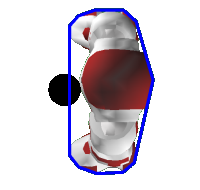
\includegraphics[scale=0.7]{figs/holding1} &
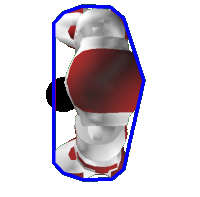
\includegraphics[scale=0.7]{figs/holding4}
\end{tabular}}

\caption{Examples for ``Ball Holding''. The black circle is the ball, the blue polygon visualizes the convex hull of the robot's projection onto the ground and the red area shows the occupied portion of the ball. Situations a) is legal, whereas b) violates the rule.}
\label{fig:holding}
\end{figure}

Intentional continual holding is prohibited even if each individual holding time does not continue for up to the time limit. In general, robots should release the ball for approximately as long as they were holding it to reset the clock. Without a sufficient release, the continual holding is regarded as a continuous hold from the very beginning and the holding rule is strictly applied.
%The violation of this rule will result in the standard removal penalty (see Section~\ref{sec:removal_penalty} for details).


\subsubsection{Exceptions to the Ball Holding Rules}
\label{sec:situations_no_ball_holding}

The following define situations where ball holding does not apply:

\begin{enumerate}
\item Ball holding may not occur when the ball becomes stuck between a robot's legs.  In such a situation, the head referee should call `clear ball' and an assistant referee should remove the ball and place the ball approximately where it was before it became stuck.
\item Ball holding may not occur when a robot falls on a ball.  The robot will either get-up and hence free the ball, or the robot should be removed under the Fallen Robot rule.
\end{enumerate}

\subsection{Player Stance}
\label{sec:player_stance}

Robots are not allowed to stay in a stance that is wider than the width of the robot's shoulders for more than 5 seconds. The robot is allowed to go into a wide stance as long as it comes back to a normal stance within 5 seconds. Staying in a wide stance for longer than 5 seconds will result in the standard removal penalty. If the robot has fallen down, it must start getting up within 5 seconds.

\subsection{Player Pushing}
\label{sec:player_pushing}

% basic definition of pushing
\emph{Pushing} is a forceful contact with another robot\footnote{This includes robots that are getting up or lie on the field.}, \ie, enough to destabilize it, and is not allowed. In the following, exceptions to this rule are specified in more detail.
The head referee will call ``Pushing \textless robot\textgreater''.

If the ball moves significantly as the result of pushing, then it should be replaced to where it was at the time of the infraction.

A Pushing Free Kick is awarded against the robot penalized for pushing if the robot is near the ball (approximately within 0.5m of the ball).

\subsubsection{Exceptions to the Pushing Rules}
\label{sec:situations_no_pushing}

The following define situations where pushing does not apply:

\begin{enumerate}
  \item Pushing may occur \textbf{only} between players of different teams.
  \item A stationary robot cannot be penalized for pushing, including a robot that is kicking, provided that the ball was close enough where a kick could have succeeded at the start of the kick motion.
  \item A robot currently getting up cannot be penalized for pushing.
  \item The goal keeper cannot be penalized for pushing while looking at or chasing the ball in it's own penalty area.
  \item Front to front contact between robots with the ball between them does not constitute pushing.
  \item Any robot proceeding to the ball whose side (\ie arm, shoulder etc.) makes contact with another robot cannot be called for pushing, Even if the second robot is not proceeding to the ball.
  \item A robot pushed by another robot can not simultaneously be called for pushing itself.
\end{enumerate}

\subsection{Playing with Arms/Hands}
\label{sec:hand_ball}

Playing with arms/hands occurs when a field player (including a defender) or a goal keeper outside its own penalty box moves its arms/hands to touch the ball (except during a fall or get-up). A robot playing with arms/hands will be subject to the standard removal penalty and the ball will be replaced at the point where it contacted the arms/hands of the offending robot.  If an own goal is scored as a result, the goal should count and the player should not be penalized.

Accidental playing with arms/hands when a robot falls or executes a get-up routine will not be penalized. If the ball goes out of play in this case, normal kick-in rules will apply (\cf Section~\ref{sec:kick_in}). However, goals (except for own goals) resulting from a ball contact with the arms/hands during a fall or get-up do not count and result in a Goal Kick (\cf Section~\ref{sec:free_kick}) as if the ball went over the goal line next to the goal.

\subsection{Leaving the Field}
\label{sec:leaving_field}

A robot that intends to leave the \TotalWidth $\times$ \TotalLength carpeted area will be subject to the standard removal penalty (\cf Section~\ref{sec:removal_penalty}).
The head referee will call ``Leaving the Field \textless robot\textgreater''.

Additionally, a robot will also be subject to the standard removal penalty where:
\begin{itemize}
\item the robot walks into the goal posts or goal net for more than 5 seconds, this includes robots that are stuck on the goal posts and unable to free themselves
\item the robot's finger become entangled in the net (without any time constraint).
\end{itemize}


\subsection{Jamming}
\label{sec:jamming}
During the match, any robot shall never jam the communication and the sensor systems of the opponents:

\begin{description}

\item[Wireless communication.] Each robot is only allowed to send a limited number of UDP messages that have to comply with a predefined format (\cf Section~\ref{sec:wireless}). If a robot uses a different protocol or sends too many messages over a couple of seconds in a game, it will be disqualified for that game. If a team violates this rule in multiple games, disqualification from the tournament (including technical challenges as well as the drop-in competition) as well as an entry in the penalty list will be the consequence. Except for the wireless cards and the access points provided by the organizers of the competition, nobody close to the field is allowed using 2.4~GHz radio equipment (including cellular phones and/or Bluetooth devices).

\item[Whistle interference.] Both the teams and the audience shall avoid intentionally confusing the robots by producing similar sounds to the game whistle.

\item[Acoustic communication.] If acoustic communication is used by both teams, they shall negotiate before the match how they can reduce interference. If only one team uses acoustic communication, the robots of the other team shall avoid producing any sound. In addition, both the teams and the audience shall avoid intentionally confusing the robots by producing similar sounds to those used for communication.

\item[Infrared communication.] If infrared communication is used by both teams, they shall negotiate before the match how they can reduce interference (if at all). Both the teams and the audience shall avoid confusing the robots by producing similar infrared signals to those used for communication.

\item[Visual perception.] The use of flashlights is not allowed during the games.  However, flash photography from the audience is allowable as long as the head referee believes the purpose of the flash is not to jam any of the robots.

\end{description}

\newpage

\section{Judgment}

The referees are the only persons permitted on the carpeted area (\ie the field and the border area).

\subsection{Head Referee}
\label{sec:head_referee}

The head referee is in charge of the game. Any decision of the head referee is valid. The head referee's decision is final and can not be changed afterwards, even by video proof. There is no discussion about decisions during the game, neither between the assistant referees and the head referee, nor between the audience or the teams and the head referee.

The head referee announces decisions by a clear loud call, and (as required) whistle sound.
The whistle, or where there is no whistle the first verbal word of the referees calls, defines the point in time at which the decision is made.
The referees should make efforts to use consistent and clear calls, and it is preferable for referees to use the calls as specified in these rules\footnote{The calls specified in these rules are detailed in English. With the agreement of the teams, the referees may use suitable calls in any language. The exception to this are technical challenge(s) that depends on the calls as specified. The use of consistent calls is also in preparation for future changes~(\cf Section~\ref{sec:future_changes})}.
The intention of specifying the referee calls is for clarity and consistency across games.

Where a whistle is required, the head referee first whistles and then announces the reason for the whistle.
The head referee may choose to use any normal sports whistle.
Each whistle sound should be short and not too loud as to interfere with other fields and simultaneous games.
The head referee must \textit{only} sound the whistle in circumstances described in these rules.
There are three circumstances when the whistle is sounded, Kick-off~(\cf Section~\ref{sec:kick-off}), a goal~(\cf Section~\ref{sec:goal}), and ending a half of gameplay~(\cf Section~\ref{sec:game_struct}).

The head referee should avoid handling the ball (except for placing a ball for kick-off), and avoid handling the robots.
Their duty is to monitor and adjudicate the game.
The head referee should only handle robots and the ball if absolutely necessary to expedite gameplay or removal of penalised robots, where the assistant referees are otherwise occupied or too far away.

\subsection{Assistant Referees}
\label{sec:assist_referee}
The two assistant referees handle the robots and the ball. They start the robots if the wireless is not working, they move the robots, if manual placement is requested, they take the robots out when they are penalized, and they put the robots in again. If a team requests to pick up a robot, an assistant referee will pick it up and give it to one of the team members once the head referee approves. An assistant referee will also put the robot back on the field. An assistant referee will also replace the ball when it goes off the field or becomes stuck between a players feet.

The assistant referees can \textit{indicate} violations against the rules committed by robots to the head referee, so that the head referee can decide whether to penalize a certain robot or not. Assistant referees should only enter the field to execute a decision made by the main referee. They should not prevent robots from falling during the game.

\subsection{Operator of the GameController}
\label{sec:gameControllerOp}
The operator of the GameController sits at a PC outside the playing area.
As with the head referee, the operator should make efforts to use consistent and clear calls.
They will signal any change in the game state to the robots via the wireless as they are announced by the head referee.
Note that for both kick-offs and goals, the moment of whistling is determining, not the verbal announcement of the head referee.
The operator will also inform the assistant referees when a timed penalty is over and a robot has to be placed back on the field.
They should announce when the ball is in play on kick-off by stating ``Ball Free'', if the \KickOffBallFreeTime time period has elapsed in the playing state.
They are also responsible for keeping the time of each half (\ie, they stop the clock after a goal or game stuck, and continues it at the kick-off\footnote{The clock may not be stopped during the preliminaries.}).
They should count aloud the remaining seconds in a half once the time remaining is 5 seconds or less.
Finally, they should repeat the calls of the head referee to make sure it was heard correctly.

\subsection{Referees During the Match}

The head referee and the assistant referees should wear clothing and socks \emph{of black or dark blue color} (blue jeans are acceptable) and avoid reserved colors for the ball, the goals, and player markings in their clothing. They may enter the field in particular situations, \eg, to remove a robot when applying a penalty. They should avoid interfering with the robots as much as possible.

\subsection{A Remark on Artificial Landmarks}
\label{sec:judgment:landmarks}

The head referee may decide at any point before or during a game to relocate any objects around the field, or direct persons to another position around the field.

The intent of using same-colored goals is to remove artificial landmarks.
Robots should be able to localize with the SPL field and its ``normal'' surroundings.
Introducing new team-specific artificial landmarks is against the spirit and intention of the league's progress.
The application of this rule needs to be well considered and should be reserved for situations which seem constructed by one team or another, but will ultimately be the head referee's decision alone.

\newpage


\appendix

\section{The Official RoboCup Competition Rules}
\label{sec:comRules}
This section contains rules that are not directly relevant for games and that may not apply at local opens.  However, these rules will be upheld at the yearly international RoboCup competition.

\subsection{Qualification Procedure and Code Usage}
\label{sec:qualification_procedure_codeuse}

The qualification procedure as well as the corresponding deadlines will be announced by the Technical Committee before qualification applications are accepted.

The RoboCup Standard Platform League offers unique possibilities to use code from other teams. In spirit of the RoboCup every team is generally allowed to use code from other teams to push the league further with their own research.
This use must be cited.
However, every participant of RoboCup \textbf{\textit{has a duty}} to contribute to the league.

To qualify, every team must make at least \textit{novel contribution} within their soccer software.
A team must have made at least one contribution within the last \NovelContributionTime.
Contributions outside of this period are no longer considered sufficiently novel and a team must make at least one \textit{new} contribution.
It is also \textit{mandatory} for a team to use their novel contribution in all competition games.
A novel contribution is:
\begin{itemize}
  \item Research publishable contribution to a \textit{game critical module}
  \item Complete replacement of a \textit{game critical module}, with original software. This may not necessarily be necessarily research publishable, but must be of equivalent scale and quality to research publishable work.
\end{itemize}

It is not a novel contribution to replace a module with code copied from another source, or to simply train a machine-learning model released by another team using new data.

As of the 2022 competition, the following are recognized as game critical modules:
Ball detection, Robot detection, Robot vision (not otherwise listed), Localization, Walk/Kick engine, Dynamic stabilization, Behavior Architecture, \& Distribution computation, Whistle detection.

As of the 2022 competition, the following are \textit{not} recognized as sufficiently game critical (even if the ability to play soccer depends on these):
Hand-written Soccer Behaviors, Natural Language detection, \& Robot and GC Communication.

In their qualification application, teams may petition the technical committee to recognize other novel contributions not listed here.
Additionally, a team that has participated at RoboCup for at least \NovelContributionTime consecutively may petition the technical committee to recognize contributions to non-game critical modules, such as developing infrastructure for the league\footnote{However, the technical committee should balance whether a team is continuing to use their own software in games.}.
A team may also petition for the technical committee to reconsider the list of game critical and non-game critical modules.
Successful petitions will be public ally announced to the league for transparency.
%For example, a team may petition and provide evidence that their work on the whistle detection is substantial and game critical, thus satisfying the requirements of a novel contribution.

If a team that is otherwise eligible for qualification cannot provide sufficient evidence of the required contributions by the deadline for applications, then that team may be qualified for RoboCup \textit{on probation}.
In this case, the team must provide evidence of the required contributions to become \textit{fully} qualified by the registration deadline of the RoboCup event.
If no suitable evidence is provided, the team's probationary qualification will lapse.

Every applicant must also bring a poster containing the team's contribution, focused on the current year, to the RoboCup event to share their contributions with the other teams.

Failure to meet any of these requirements will result in a qualification penalty for subsequent years.

\subsection{Game Structure}

The clock stops during stoppages of play (such as ready and set state after goals) from the quarter-finals onward.  In round robin pool play, a game can finish in a draw as no penalty shoot-out will follow. In the promotion round, intermediate round, quarter finals, semi finals, 3rd place or final, a game that ends in a draw will be followed by a penalty shoot-out (see Section~\ref{sec:penalty_shoot-out}).

\subsection{Winner and Rankings}
\label{sec:rankings}

The team which scored more goals than the other is the winner of the match. If the two teams scored the same number of goals, the game will be a draw. The draw will follow the same system defined in Section~\ref{sec:game_struct}. Total (and final) standings will be decided on points as follows (the points will be given based on the result of each game):

\makebox[\columnwidth]{ \hfill Win = 3 pts\hfill Draw = 1 pt \hfill
Lose = 0 pts\hfill }

If a team's obtained points is the same as another team's after a round of pool play is complete, the following evaluations will be applied in order to qualify the finalists.

\begin{enumerate}

\item The points obtained

\item The difference between goals for and goals against per game

\item The average goals for per game

\item Game result between the teams directly

\end{enumerate}

\subsection{Champions Cup and Challenge Shield}
\label{sec:twoCompetitions}
In order to provide better matched games for teams of all abilities the RoboCup Standard Platform League shall be divided into two separate competitions: the Champions Cup for the strongest teams and the Challenge Shield for all other teams. Final assignment of teams to each competition occurs at RoboCup based on initial game performance.

There are 24 qualified teams.

All teams who qualify for participation in the RoboCup SPL are ranked using the Glicko system\footnote{\url{http://www.glicko.net/glicko/glicko.pdf}} based on all available results from previous official RoboCup tournaments. (New teams will be ranked equally below all previously competing teams. Teams that participated previously but did not participate in the previous year will be ranked above new teams but below teams that competed in the previous year.) The top 12 teams (by rank) will be Champions Cup candidates and the remaining teams will be Challenge Shield candidates.

All Champions Cup candidates play a single qualifier round-robin stage comprising 4 groups of 3 teams each. All Challenge Shield candidates play a similar qualifier round-robin stage also consisting of 4 groups of 3 teams each. Each Champions Cup qualifier group will consist of one team ranked 1-4, one team ranked 5-8, and one team ranked 9-12. Each of the teams ranked 13-16 will be placed in a different Challenge Shield group. Remaining Challenge Shield qualifier group places will be filled by random selection from teams ranked 17-24.

The top 2 teams in each Champions Cup qualifier group proceed automatically to the Champions Cup proper. Similarly, the lower 2 teams in each Challenge Shield qualifier group proceed automatically to the Challenge Shield. The 4 remaining Champions Cup candidates (losers in each group) play the remaining Challenge Shield candidates (winners in each group) in the so-called promotion round and the winners of these games go to the Champions Cup while the losers go to the Challenge Shield. Thereafter, the Champions Cup and Challenge Shield competitions shall proceed independently of each other and each will normally consist of a round-robin stage, followed by an intermediate round and a knockout competition. In the intermediate round the second and third placed team of each group coming from the second round-robin will play against a team from another group for a spot in the quarter-final.

\subsection{Referee Selection and Requirements}
\label{sec:refSelection}
During pool play, the games will be refereed by members of teams from a different pool.

Each team has to referee a number of games. A schedule will be released specifying the games for which each team is required to provide two referees. Referees should report to the appropriate field at least five minutes before the game is scheduled to start.

If a team fails to provide two referees for a game in which they are scheduled to provide referees, it will be noted by the organizing committee and recorded as a \textbf{qualification penalty} (Section~\ref{sec:qualificationPenalties}).

For each of the games, a team will be required either to provide the head referee and the operator of the GameController, or the two assistant referees.  The two teams assigned to referee a game shall decide among themselves which roles each team will fulfill. Note, however, that the head referee and the GameController should always be from the same team.

A team may swap their scheduled refereeing duties with another team, but the team listed on the referee schedule will be held accountable if referees fail to appear for a game they are scheduled to referee.

The requirement to referee may be an extreme hardship for extremely small teams.  If a team believes providing two referees for games will be an extreme hardship, they must send an email explaining their situation to the Organizing Committee and Technical Committee at least two weeks before the first set up day of the competition.  The Organizing and Technical Committees will then consider the request and attempt to find an acceptable solution.

Referees must have good knowledge of the rules as applied in the tournament, and the operator of the GameController must be experienced in using that software. Referees and the GameController should be selected among the more senior members of a team, and preferably have prior experience with games in the RoboCup Standard Platform league.

In each game, each of the teams playing shall be able to veto one and only one eligible referee with no reason required.


\subsection{Subsequent Year Pre-Qualification Procedure}
\label{sec:preQual}
Up to 11 teams may become pre-qualified for the subsequent year's team competition by fulfilling one of the following criteria:
\begin{itemize}
    \item Reaching the quarter-finals of the Champions Cup
    \item Reaching the final of the Challenge Shield
    \item Being the team with the best overall result in the technical challenges that is not pre-qualified by other means, and finishing at worst 5th in the technical challenges.
\end{itemize}

However, pre-qualified teams must do all the following in order to remain pre-qualified:
\begin{itemize}
\item Post in a publicly available location a team research report describing their work for the 2019 competition
\item Publicly release code from that year's codebase, either in the form of a complete release (perhaps without behavior) or limited libraries.  This release must be documented and coded in a way where it can be used by others.
\item Submit a shortened application as required by the call for participation for the subsequent year's competition.
\end{itemize}

\subsection{Qualification Penalties}
\label{sec:qualificationPenalties}

There are a number of offenses which lead to qualification penalties being recorded against a team. These are as follows:
\begin{itemize}
    \item Withdrawing from RoboCup after the final commitment deadline
    \item Failing to referee when assigned (Section~\ref{sec:refSelection})
    \item Forfeiting a game (Section~\ref{sec:forfeit})
\end{itemize}

A team cannot be pre-qualified for RoboCup in the year following a qualification penalty. Furthermore, a qualification penalty is considered by the Technical Committee when reviewing applications and will negatively affect the assessment of a team's application. Multiple penalties accumulate and will result in an even more negative assessment of a team's application. Qualification penalties are considered for a period of three years following the offense.

Whenever a qualification penalty is recorded, all relevant details including any possible mitigating circumstances are also recorded and these will also inform the assessment of a team's application.

\subsection{Disqualification during Competition}
\label{sec:disqualification_during_comp}

A team may be disqualified during the RoboCup competition for:
\begin{itemize}
  \item A serious violation of the terms of a team's qualification
  \item Gaining a Qualification Penalty during the course of the competition~(\cf Section~\ref{sec:qualificationPenalties})
  \item A serious breach of ethics, or serious behavior unbecoming of participants of RoboCup.
\end{itemize}

\textbf{Example.} A team promises to use their novel contribution in RoboCup games, but fails to do so.
Alternatively, a team deliberately misleads the technical committee about the novelty of their work and/or their contribution to the league, such that they are deemed to have copied another team.

A team can \textit{only} be disqualified by a decision of the \textit{Board of Trustees of the RoboCup Federation}.
The RoboCup Soccer SPL executive must petition the board in writing at their soonest possible availability.
The executive must simultaneously inform the relevant team of the petition in writing.

A disqualified team automatically forfeits all games~(\cf Section~\ref{sec:forfeit}).
For practicality, the disqualification should not apply \textit{retroactively}.
However, by majority vote of the team leaders, provisions for retroactive disqualification may be made in the fairness of the affected teams.

\newpage

% !TeX root = ../SPL-Rules.tex
% !TeX spellcheck = en_US
\section{Technical Challenges}

\subsection{7 vs. 7}
    This competition extends the ideas from the mixed team competition, and 1 vs. 1 remote challenge from RoboCup 2021 to a standardized 7 vs. 7 on-site competition. Another goal is to enforce more collaborative game play. This challenge will only be executed if at least four teams participate.

    \subsubsection{Condition for participation}
    \label{sec:7vs7:condition_for_participation}
        \begin{itemize}
            \item A 7 vs. 7 team can be build from a single team but also from multiple teams.
            \item Teams need at least four own robots to play with.
            \item Teams have to provide three tested robots (\textbf{only V6 version}) to a robot pool.
            \item The pool robots have to be calibrated in limited time.
        \end{itemize}

    \subsubsection{Rules}
        This challenge bases on all rules from the 5 vs. 5 competition (\crefrange{sec:setup_environment}{sec:judgment}). The following list contains extended and changed rules for this challenge in order to ensure, among other things, the safety of pool robots:

        \paragraph{Players}
            In total each team consists of 7 players without a substitution robot. The 7 robots consist of 4 own and 3 pool robots. Whereby the pool robots are only V6s. Each jersey shirt has therefore now player numbers between 1 and 7 printed on it (\cf \cref{sec:team_markers}). Also the new positions of the initial kick-off (\cf \cref{sec:initial-kick-off}) for 7 robots can be seen in \cref{fig:initial_positions_7vs7}.
            \begin{figure}[t!]
            	\begin{center}
            		\leavevmode
            		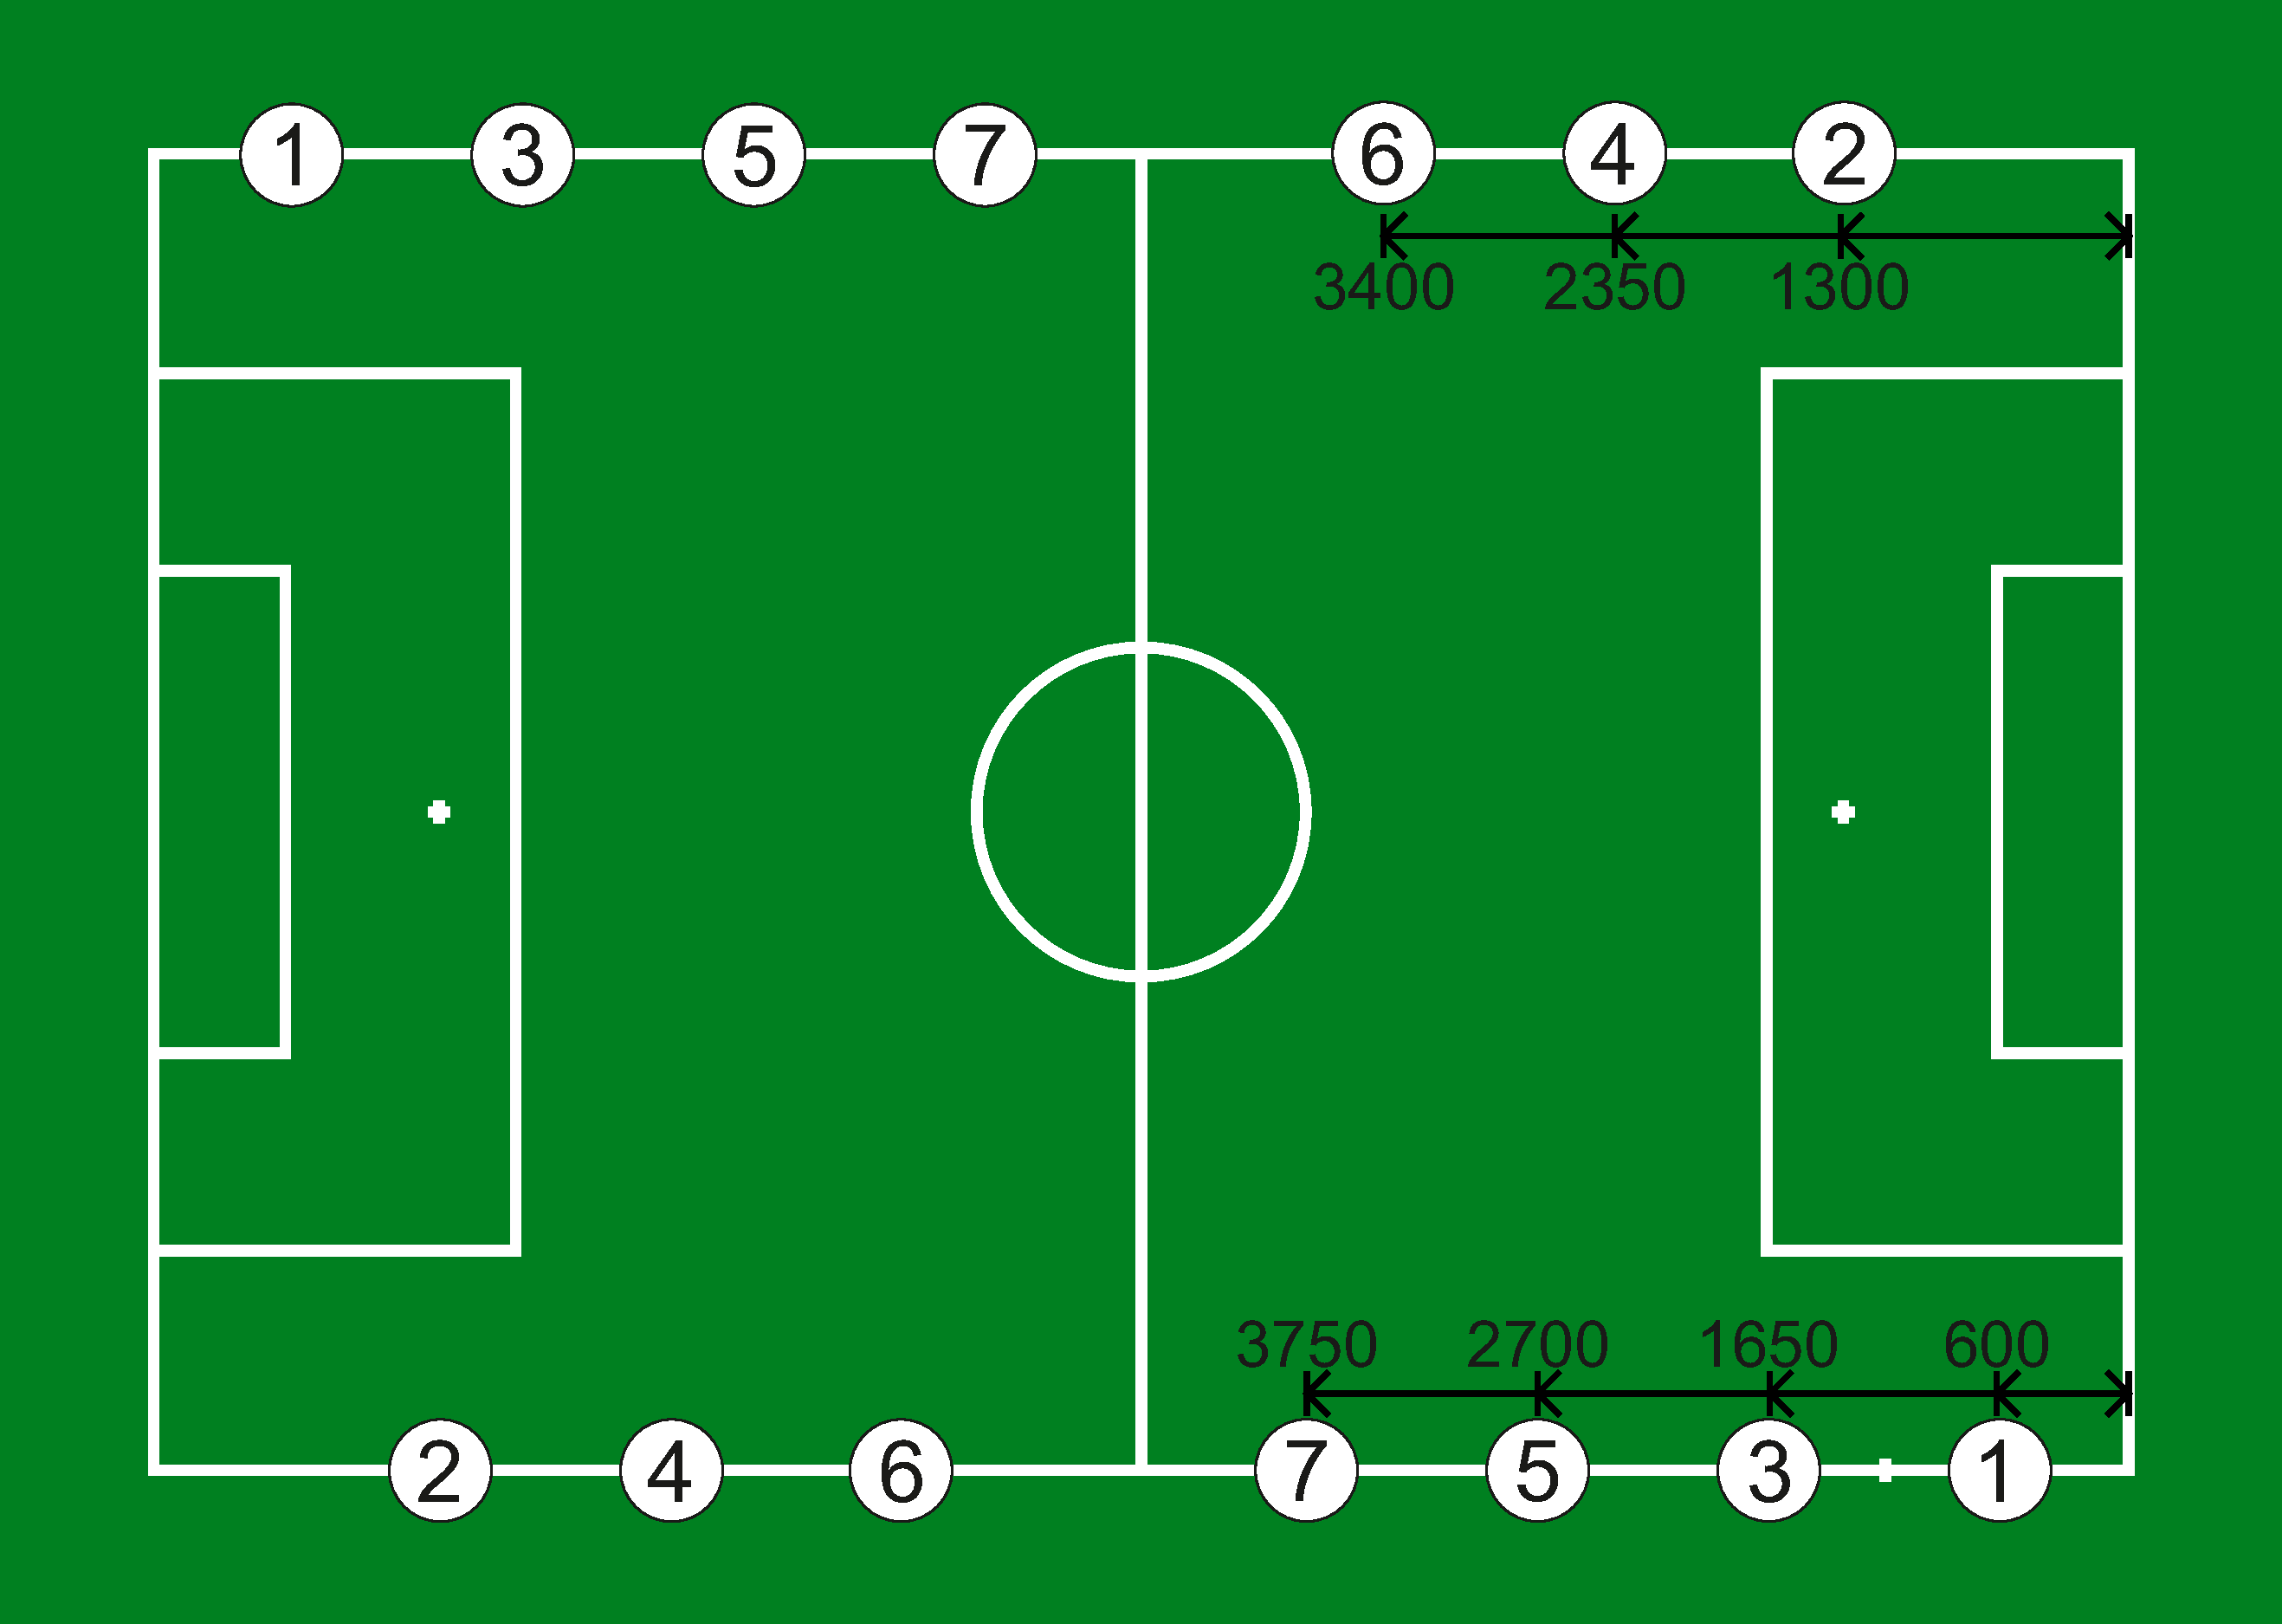
\includegraphics[width=1\columnwidth]{figs/initial_positions_7vs7.pdf}
            		\caption{Positions, player numbers and distances from the center of the goal line for the initial kick-off of the 7 vs. 7 robots.}
            		\label{fig:initial_positions_7vs7}
            	\end{center}
            \end{figure}

        \paragraph{Referees}
            \label{sec:7vs7:referee}
            All referees are allowed to prevent robots from crashing to the ground by catching them beforehand and then laying them down gently. Additionally the head referee decides whether a robot excessively damages itself and should remove it from the field via a forced “Request for Pick-up”, \cf \cref{sec:request_for_pickup}.

        \paragraph{Robot Pool}
            Each team has to contribute at least 3 robots to the robot pool, \cf \cref{sec:7vs7:condition_for_participation}. If a team cannot provide enough own robots and there are still functional robots in the robot pool, then this team can get more than the 3 robots from the pool to restock up to 7 robots. However, the final decision is still up to the head referee. \\
            The robot pool exists only virtually, so that there is no central location where all pool robots are stored. Each team is also allowed to use their own pool robots when they are not in use. However, each pool robot gets a unique ID and in order to be able to recognize the pool robots visually, a sticker is attached to the outer sides of the upper arms and on the back of the head.

        \paragraph{Robot Pool Evaluation}
            \label{sec:robot_pool_evaluation}
            In order to guarantee that the pool robots are functional, and all parts are working within their limits each team has to provide a proof of functionality one hour before a specific pool robot is planned for a game. Also, the team has to ensure that this robot had at least a cooldown period of \qty{15}{\minute} and is charged to at least \qty{80}{\percent}.
            A common robot evaluation image will be provided by the community with a standardized setup procedure (custom image) and with automatic calibration. Afterwards the robot should walk towards a ball and shoot it. If this evaluation is completed without any problems within a given time \todo{set time} and the robot falls down less than 2 times, the evaluation is to be rated as functional. Otherwise, this robot is considered to be non-functional for the time being. Every team can propose such an image up to the 2022-06-01\todo{set deadline}, as well as additional tests which should be included in such an evaluation image. A manual how to use the custom image should also be included.

        \paragraph{Hardware Related Penalties}
            \label{sec:7vs7:hardware_related_penalties}
            Since teams are partially playing with robots from other teams, there is a maximum of two hardware related penalties for each robot in the first half and one more in the second half.
            Hardware related penalties are:
            \begin{itemize}
                \item fallen robot or inactive robot, \cf \cref{sec:fallenrobots}
                \item request for pick-up in the playing or ready state — either by the team or forced by the head referee, \cf \cref{sec:request_for_pickup} and \cref{sec:7vs7:referee}.
            \end{itemize}
            These penalties are counted by the GameController operator and after that a robot with additional hardware related penalties is excluded for the rest of the game (they are transitioned into the unstiffed state by the assistant referees, \cf \cref{sec:robot_states})!

        \paragraph{Own Pushing}
            In addition to the normal pushing rules, \cf \cref{sec:player_pushing}, pushing may now occur between any robots, i.e., also between teammates.

        \paragraph{Limited Diving}
            Pool robots are not allowed to dive for the ball on purpose, \cf \cref{sec:fallenrobots}, except for penalty kicks! In case of violation, the infringing robot will be taken out according to the forced ``Request for Pick-up'' rule, \cf \cref{sec:7vs7:referee}, and therefore counts as a hardware related penalty, \cf \cref{sec:7vs7:hardware_related_penalties}. However, this restriction does not apply to the team's own robots.

        \paragraph{Match Phases}
            Each match consists out of the following phases:
            \paragraph{Robot check} Each team marks and checks its robots sent to the robot pool as described in \cref{sec:robot_pool_evaluation} and reports its availability (1.5 hours before a match starts).
            \paragraph{Setup} One hour before the match starts, the teams receive their randomly selected robots. They have now time for set-up and calibration. For calibration only one half of the field is available for a team. The area within the center circle is not allowed to be entered by the robots until the match starts.
            \paragraph{Game} During a match additional rules apply for the pool robots. Referees are asked to try to save the robots' hardware by catching them before they crash onto the ground.
            \paragraph{After game} Teams have time of \qty{15}{\minute} to return the pool robots to the pool.

        \paragraph{Mode}
            The mode will be determined after teams have registered. At least 4 teams should register, before the challenge will be executed. The selected mode (e.g., group phase, double elimination, Swiss system tournament) will be determined after teams have registered.

\subsection{Visual Referee Challenge}

    \subsubsection{Challenge Goal}

        For the moment robots receive the decision made by the head referee either from a short whistle or a GC message. To improve the perception of the robot and to listen more to the head referee this challenge introduces visual referee signs.

    \subsubsection{Challenge setup}

        One robot of the challenged team is placed in the center circle facing the head referee standing on the T-junction opposite to the GC. The referee wears red gloves. The robot watching the referee and listening for the whistle. The general procedure is as follows:

        \begin{itemize}
            \item The referee blows the whistle.
            \item The referee shows his decision for \qty{15}{\second}.
            \item During that time or in the additional \qty{10}{\second} the robot has time to phrase the referee's decision, e.g., ```Kick-off left team'''. \todo{Or we use a TCP message}
        \end{itemize}

        This procedure will be continued for in total four times. Each time, the referee chooses a new decision.

    \subsubsection{Available Decisions}

        For each decision (not all, because some decisions have to be shown on place, e.g., throw in) will be described and pictured.

        \begin{itemize}
            \item \textbf{Kick-Off}
            \begin{figure}[ht!]
                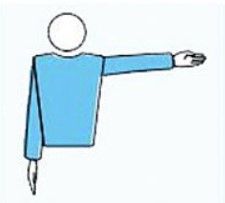
\includegraphics{figs/kick-off_referee.jpg}
            \end{figure}
        \end{itemize}

    \subsubsection{Challenge evaluation}
        The time from the whistle until the robots starts messaging will be counted for each run.
        For each decision two points can be awarded: One for the right decision itself and one for the right team awarded to or against.
        The ranking is based on the sum of points. Higher number of points leads to a higher ranking. For teams with equal points the sum of the runs will be used. Less time used leads to a higher ranking.


\subsection{Dynamic Ball handling Challenge}

    This challenge extends the idea of RoboCup 2021's Passing Challenge. The purpose of this challenge is to enhance skills in ball passing and handling, and in robot's movement estimation.

    \subsubsection{Challenge Goal}

        Score as attacking team a goal after a double pass without letting the defending players touch the ball.

    \subsubsection{Challenge Setup}

        This challenge uses a standard SPL field, with GameController and 3 attacking robots provided by the challenged team and three defending robots operating a provided common image (see \cref{sec:Challenge_image}) from another team. If more than one image exists, than multiple images will be provided and for each run a new one will be randomly selected.

        Attacking teams have to have their robots ready \qty{40}{\minute} before a run starts. Attacking robots are not allowed to be changed afterwards. Then the defending teams receive which randomly selected common image will be used. In that time the defending robots have to be flashed and calibrated.

        Since the challenge has three runs for each team, each team will be teamed with another team for a run. Both teams have to provide the same three robots (except one robot breaks) as attacking as well as defending team. Following from this each run is divided into two parts. Executed after each other.

        The robots are placed by the referees with some randomness to left or right as follows:

        \begin{description}
            \item[Attacker:] 1st: goal area front line; 2nd: next to center line left of center circle; 3rd: next to center line right of center circle
            \item[Defender:] 1st: within center circle; 2nd: front line penalty area; 3rd: goalkeeper in the middle between the two goal posts. Defending robots are limited to a maximum speed of \qty{20}{\cm \per \second}.
            \item[Ball:] On penalty spot of the attacking team's side
        \end{description}

        \begin{figure}[t!]
            \begin{center}
                \leavevmode
                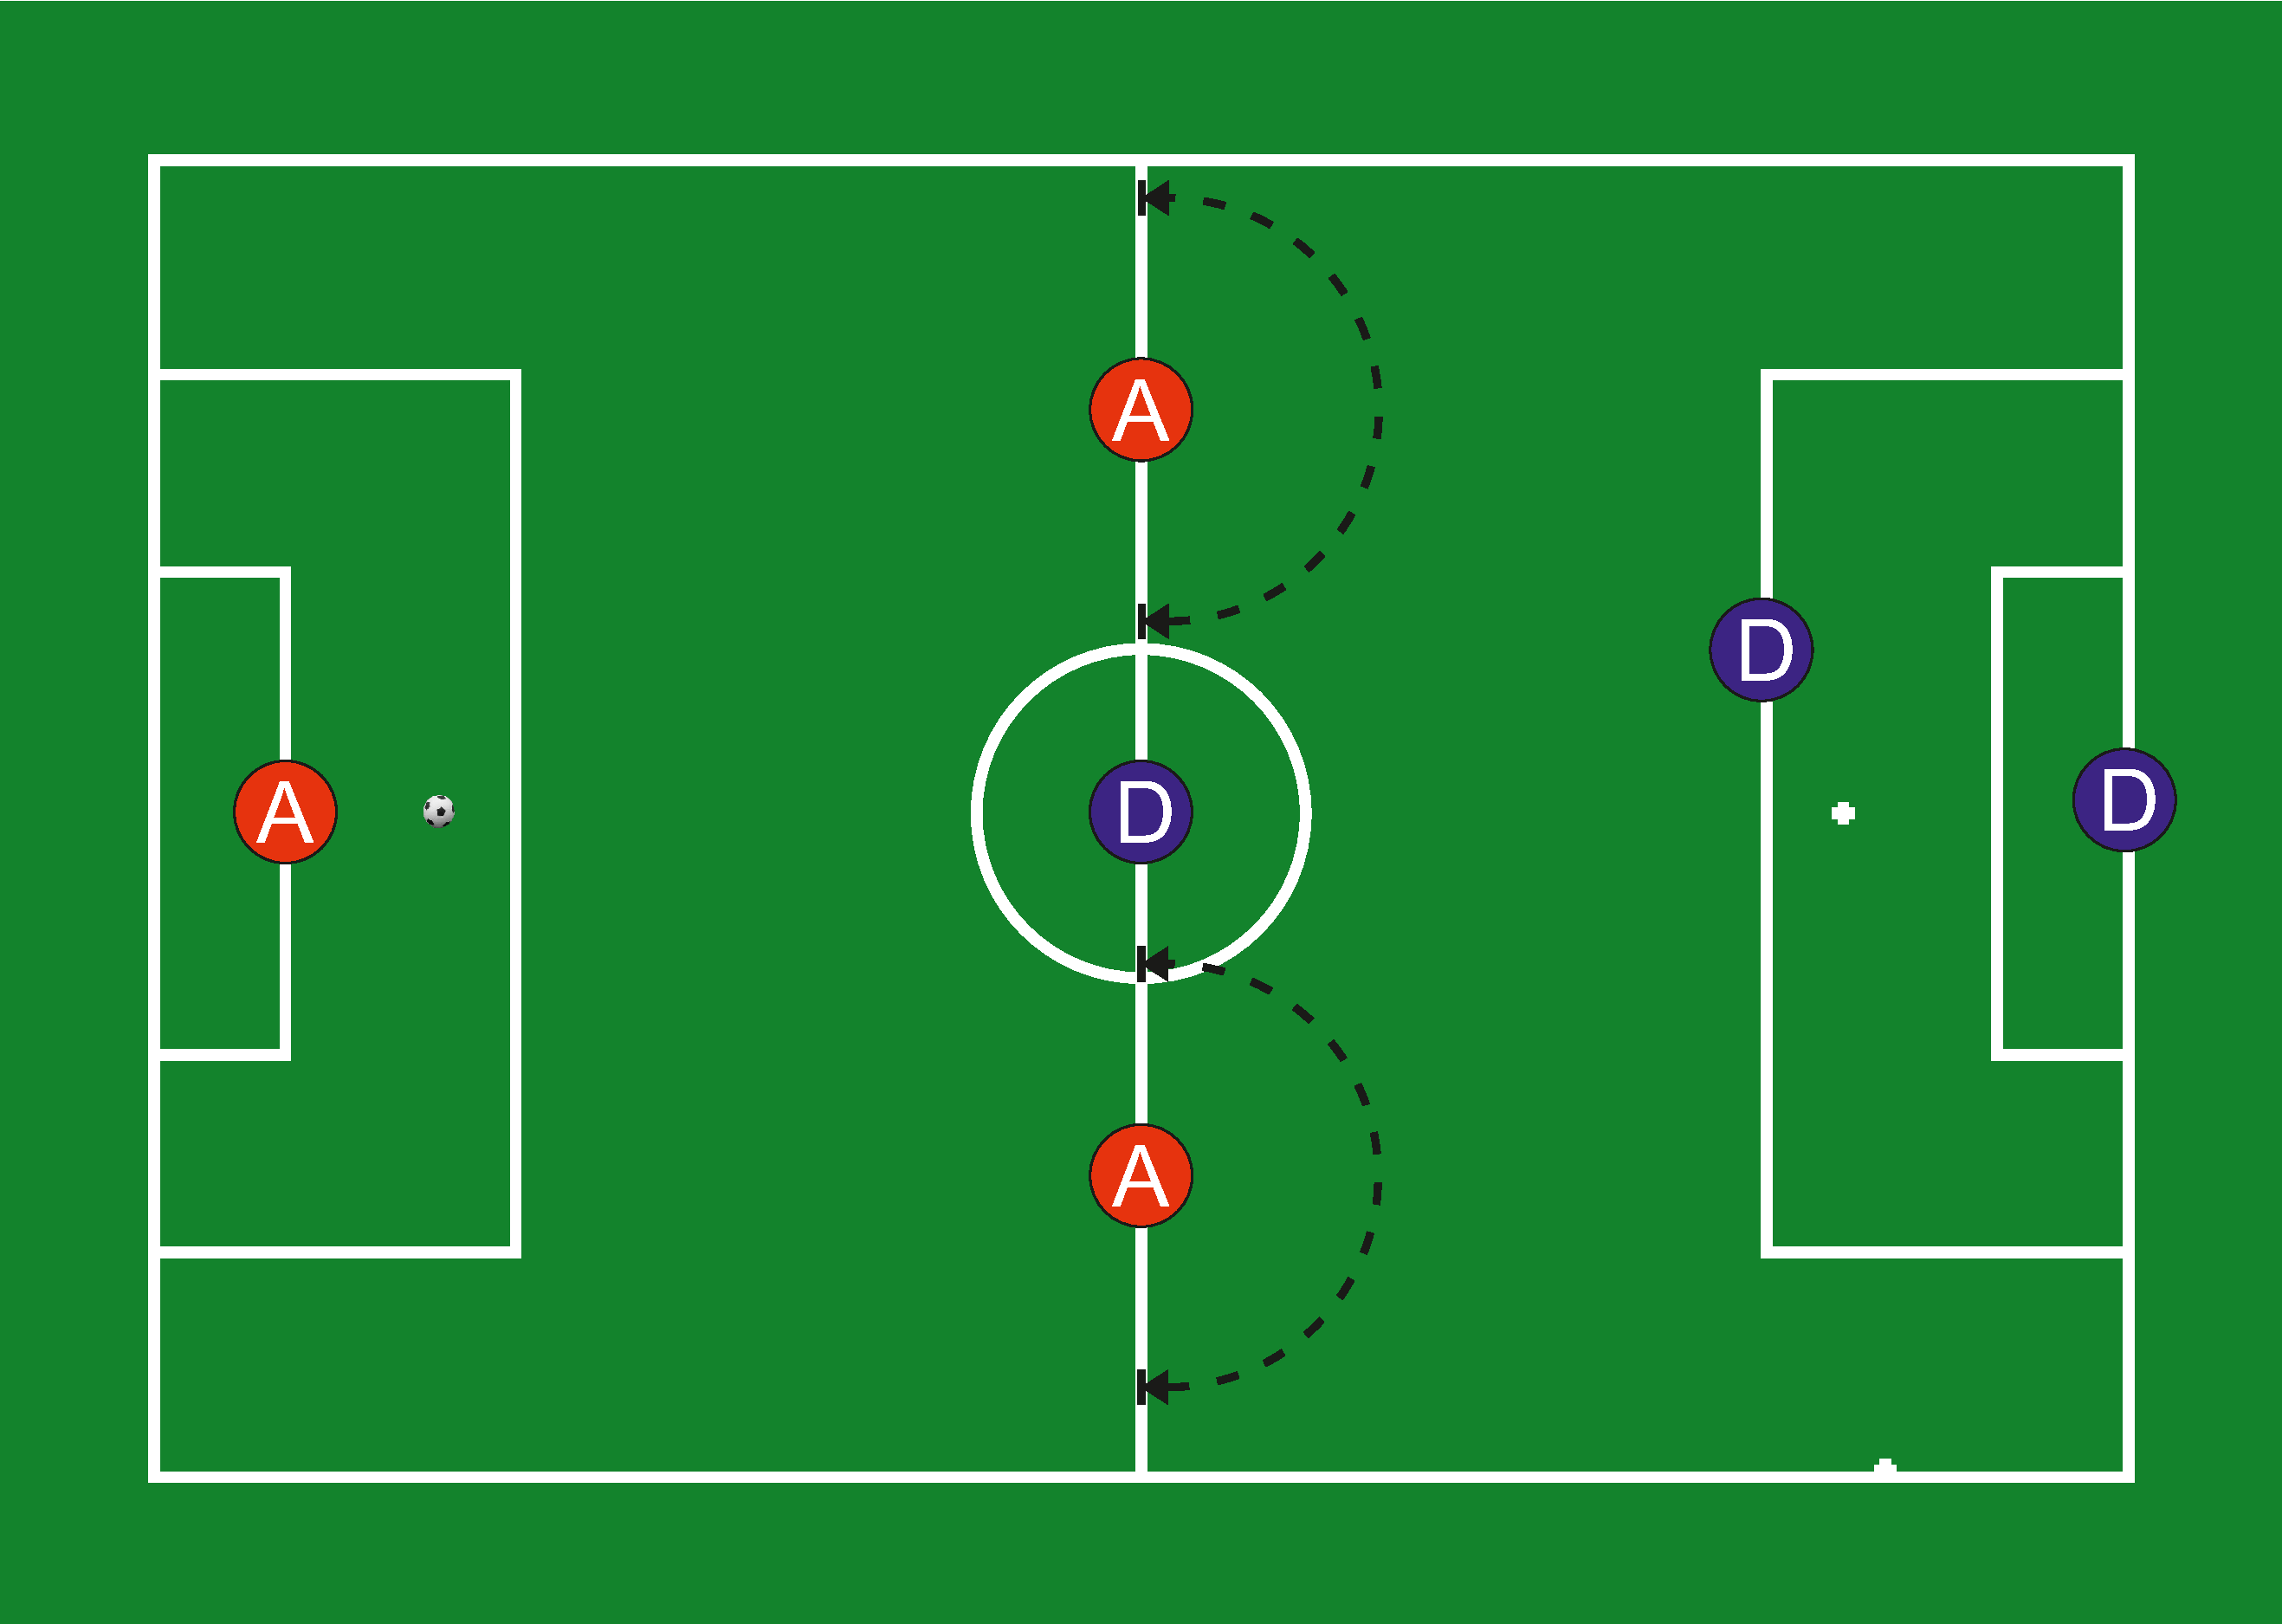
\includegraphics[width=1\columnwidth]{figs/ball_handling_positions.pdf}
                \caption{Possible positions of the attacking (red) and defending (blue) robots at the beginning of the challenge. The black semicircle indicates the area in which a pass is valid.}
                \label{fig:ball_handling_positions}
            \end{center}
        \end{figure}

    Each team has three attempts to run this challenge.

    \subsubsection{Challenge Execution}

        All six robots have to be in the Wi-Fi. In \texttt{initial} the robots get placed at their randomized starting positions. GC goes from \texttt{ready} directly into \texttt{set}. The ball gets placed, and the head referee starts the challenge execution with one whistle, like at kick-off. If a robot does not listen to the whistle, it will get the delayed \texttt{playing} signal from the GC.

        In \texttt{playing} the following happens: The 1st attacker plays the ball towards the 2nd or 3rd attacker while he is under attack by the 1st defender.
        A pass counts as a valid pass if the ball stops in front of the receiving robot towards the opponent's goal. The ball has to stop in the vicinity of the receiving robot (at max \qty{1}{\metre} distance between receiver and ball, see~\cref{fig:ball_handling_positions}).
        The 1st defender does not walk back in its own half and the goalkeeper remains on the goal line and is not allowed to dive. The objective of the defending team is to intercept the passes, see stopping criteria.

        After the 2nd or 3rd attacker received the ball, and the ball is in the defender's half, it gets attacked by the 2nd defender. The task of the 2nd or 3rd attacker is now to pass towards the 3rd or 2nd attacking robot, which than shots onto the goal.

        If a defender pushes an attacking robot, the attacking team gets a time bonus of \qty{15}{\second} and the pushing robot will be removed from this run.

    \subsubsection{Challenge Scoring}

        For each run the referee measures the execution time from initial whistle until the run is stopped by one of the following criteria:

        \begin{itemize}
            \item A defender touches the ball.
            \item Ball leaves the field.
            \item An attacker pushes.
            \item A run exceeds \qty{4}{\minute} execution time.
            \item A goal is scored.
        \end{itemize}

        A score for the run will be calculated based on the following rules:

        \begin{enumerate}
            \item The time measured counts.
            \item If an attacking robot has been pushed by a defender, subtract \qty{15}{\second}.
            \item If a goal has been scored after two passes, subtract \qty{30}{\second}.
            \item If a ball has been passed wrongly, add \qty{10}{\second} for each incorrect pass.
            \item If the ball got touched by the 1st or 2nd defender, execution time will be \qty{240}{\second}.
            \item If the ball leaves the field not from inside the defending goal area, execution time will be \qty{240}{\second}.
            \item If an attacking robot has pushed, execution time will be \qty{240}{\second}.
        \end{enumerate}

        The final result is the mean time out of three runs.

    \subsubsection{Challenge image}
        \label{sec:Challenge_image}
        \todo{Deadline for submission}
        A common image will be provided by the community with the standardized setup procedure and with automatic calibration. Every team can propose such an image \todo{deadline}. The image will be tested if they match the requirements.
        \todo{Criterias for images, how to setup}

\subsection{Open Research Challenge — Video analysis / statistics}
In order to evaluate the progress of the league, regardless of the annual rule changes, we need statistics similar to human soccer. Therefore, only GameController/TeamCom statistics are not sufficient for this. That's why there is an Open Research Challenge, as already known from the year 2019 (and previously until RoboCup 2014), which will focus on the generation of statistics from external video data from a go-pro type camera viewpoint.

    \subsubsection{Challenge Goal}
    For this Open Research Challenge two major goals exist. The more short-term goal is to calculate extrinsic camera parameters (camera matrix) from the camera feed and to locate/track all moving objects (ball, robots) on the field. In addition to this, the more long-term goal involves the creation of game statistics based on the located objects and positions from the short-term goal. Here, the following statistics, among others, might be of interest, such as time under control, shots on goal (successful/unsuccessful), passes and so on. Since this is an open challenge, the decision of what to show (short-term, long-term, parts of it) is, within the scope of the goals aforementioned here, entirely up to the teams. In addition, the execution time for this challenge is also not relevant for the time being whether you process it online or offline to the video stream.

    \subsubsection{Condition for participation}
    \begin{itemize}
    \item In order to compete in this Challenge, teams must notify the TC (\url{rc-spl-tc@lists.robocup.org}) of their interest in participating by 2021-12-31, at the latest.
    \item Subsequently, all participating teams will receive a pre-processed video from the RoboCup2019 (i.e. a sequence of images) and have to label it according to the enclosed instructions. Annotating must be completed by 2022-02-01 to in order to form a shared ground truth data set. However, the final format in which the teams have to submit their annotations has not yet been determined, but the TC is happy to accept suggestions. Also the exact details are given to the teams together with the to be labelled data set.
    \item With this shared ground truth data set, teams can then implement their own approach/ideas. Also any failures in the annotations can be corrected by the community/teams since the data will be shared on the SPL Github\footnote{https://github.com/RoboCup-SPL}.
    \item The teams have to create a poster (A3/A2/A1 size\todo{decide the size}) for the RoboCup 2022 showing their results and prepare a short 3 minutes oral presentation which additionally explains and shows the idea and results of this approach.
    \item All teams are requested to publish the code for their approach to enable a fast progress of the league in this area. However, only the top 3\todo{decide the number} ranked teams are required to publish their code within one month after the RoboCup 2022.
    \end{itemize}

    \subsubsection{Scoring}
    The winner will be decided by a vote among the SPL teams using the Borda count mechanism (\url{http://en.wikipedia.org/wiki/Borda_count}). Each participating SPL team will vote for their top 5/10\todo{decide the number} teams in order (excluding themselves). Teams are encouraged to evaluate the performance based on the following criteria: achievement of the long/short-term goal, execution time, accuracy/precision/recall, technical strength, novelty. At a time decided by the designated referee, within one hour of the last demonstration if not otherwise specified, the captain of each team will submit the team's rankings by filling out an online form. Any points awarded by a team to itself will be disregarded. The points awarded by the teams will be summed and thus form the score of this challenge which is then converted according to the formula described in the beginning of this section.

    \subsubsection{Labelling}
    This section gives a brief overview of the labelling task.\\

    Input data (given):
    \begin{itemize}
        \item The assigned, pre-processed, go-pro videos/sequences from a game of the RC2019.
        \item Additionally the GC data, TeamCom logs and the intrinsic calibration of the go-pro.
    \end{itemize}

    Output data (to be annotated):
    \begin{itemize}
        \item Calculation of the extrinsic camera parameters (camera matrix). Preferably for each frame, although this is mainly necessary when the camera was moved/wobbled. However, it should be checked at least once for each minute whether the camera matrix is still appropriate.
        \item Labelling of all robots and the (main) ball: These objects should be labeled using bounding boxes. Special attention should be paid to the bottom edge as this will be used to determine the position of the object.
        \item In addition, the robots must be labelled with their jersey colour and number.
    \end{itemize}
    Also not everything is fixed yet so that the TC is happy to accept suggestions at \url{rc-spl-tc@lists.robocup.org}.

\newpage

% !TeX root = ../SPL-Rules.tex
% !TeX spellcheck = en_US
\section{Changes From 2019}
This is a brief list of rule changes from 2019 to 2022.

\begin{itemize}
  \item General housekeeping and tidy-up of rules.
  \item Remove some duplicated items
\end{itemize}

\subsection*{Field Layout}
\begin{itemize}
  \item Increased size of the penalty box (\cf Section~\ref{sec:field_dim})
  \item Added Goalbox - as same size of the old penalty box (\cf Section~\ref{sec:field_dim})
\end{itemize}

\subsection*{Field Colors}
\begin{itemize}
  \item Removed redundant figure (\cf Section~\ref{sec:field_colors})
\end{itemize}

\subsection*{Robot Players: Hardware}
\begin{itemize}
  \item Added black Nao plating as permitted color~(\cf Section~\ref{sec:hardware})
  \item Permit tape on the battery pack~(\cf Section~\ref{sec:hardware})
\end{itemize}

\subsection*{Robot Players: Team Markers}
\begin{itemize}
  \item Teams must specify which front and back halves of jerseys are combined.~(\cf Section~\ref{sec:hardware})
\end{itemize}

\subsection*{Structure of the Game}
\begin{itemize}
  \item Specify whistle sounds for commencing and ending each half (\cf Section~\ref{sec:game_struct})
\end{itemize}

\subsection*{Robot States}
\begin{itemize}
  \item Updated states for penalty kick (\cf Section~\ref{sec:robot_states})
\end{itemize}

\subsection*{Goal}
\begin{itemize}
  \item Referee signals a goal being scored by a whistle sound~(\cf Section~\ref{sec:goal})
  \item GameController transmission of a goal being scored is delayed by \GoalScoredDelay~(\cf Section~\ref{sec:goal})
\end{itemize}

\subsection*{Indirect Kick}
\begin{itemize}
  \item Rule introduced (\cf Section~\ref{sec:goal})
\end{itemize}

\subsection*{Kick-off}
\begin{itemize}
  \item Specify location of referee whistle
\end{itemize}

\subsubsection*{Kick-off Shot}
\begin{itemize}
  \item Kick-off shot penalty removed.
  \item Kick-off Rule subsumed by the Indirect Kick Rule (\cf Section~\ref{sec:goal}), \& Invalid Goal Rule (\cf Section~\ref{sec:goal})
\end{itemize}

\subsection*{Free Kick}
\begin{itemize}
  \item Change referee phrase for ending the free kick to ``Ball Free'' for consistency with kick-off and for less confusion on  head referees during the game.(\cf Section~\ref{sec:free_kick})
\end{itemize}

\subsubsection*{Goal Kick}
\begin{itemize}
  \item Position of goal kick adjusted to the corner of the goalbox (\cf Section~\ref{sec:kick_in})
\end{itemize}

\subsubsection*{Penalty Kick}
\begin{itemize}
  \item Rule introduced~(\cf Section~\ref{sec:free_kick}).
  \item Penalty Kick procedure introduced~(\cf Section~\ref{sec:penalty_free_kick}).
\end{itemize}

\subsection*{Penalty Kick Shoot-out}
\begin{itemize}
  \item Time for Penalty Kick reduced to \PenaltyKickTime.
  \item Striker robot is placed on the edge of the penalty box~(\cf Section~\ref{sec:penalty_kick})
  \item Goalkeeper robot must remain on the goal line and on its feet~(\cf Section~\ref{sec:penalty_kick})
  \item Removed requirement for timing sudden-death penalty shots as this is no-longer used as a tie-breaker
  \item General Rules housekeeping~(\cf Section~\ref{sec:penalty_shoot-out} \& Section~\ref{sec:sudden_death_shoot_out})
\end{itemize}

\subsection*{Illegal Defender \& Position}
\begin{itemize}
  \item Illegal Defender subsumed into to Illegal Position (\cf Section~\ref{sec:illegal_positioning})
  \item Illegal Position penalties now \textit{follow} the standard removal penalty and increase in penalty time per-robot. The only exception are illegally positioned robots during the set state.
  \item Penalty box illegal positioning applies to robots from both teams (\cf Section~\ref{sec:illegal_positioning})
  \item Number of robots permitted inside the penalty box increased to 3 (\cf Section~\ref{sec:illegal_positioning})
  \item Illegal Defender subsumed into to Illegal Position (\cf Section~\ref{sec:illegal_positioning})
  \item Penalty box illegal positioning applies to robots from both teams (\cf Section~\ref{sec:illegal_positioning})
\end{itemize}

\subsection*{Leaving the Field Penalty}
\begin{itemize}
  \item Clarified leaving the field also applies to walking into the goal posts~(\cf Section~\ref{sec:leaving_field})
\end{itemize}

\subsection*{Jamming}
\begin{itemize}
  \item Explicitly define interference of whistle sounds~(\cf Section~\ref{sec:jamming})
\end{itemize}

\subsection*{Judgement - Head Referee}
\begin{itemize}
  \item Modified head referee's use of the whistle as it is now important for robots to detect the whistle during gameplay. Whistle's are only used for kick-off, end-of-half and goals.
  \item Removed whistle sound for game stuck.
  \item Added requirement to use calls as defined in the rules.
  \item Clarified head referee's role in handling robots and the ball.
  \item Removed requirement for timing sudden-death penalty shots as this is no-longer used as a tie-breaker
\end{itemize}

\subsection*{Official Rules - Qualification Procedure}
\begin{itemize}
  \item Revised qualification requirements for novel contributions and reuse of existing software~(\cf Section~\ref{sec:qualification_procedure_codeuse})
  \item \textbf{ALL TEAMS}: Note novel contribution requirements now apply to all teams.
\end{itemize}


\subsection*{Official Rules - Disqualification during competition}
\begin{itemize}
  \item Added possibility to disqualify a team during competition for serious ethical breaches, or violation of the terms of their qualification~(\cf Section~\ref{sec:disqualification_during_comp})
\end{itemize}

\subsection*{Mixed Team Tournament}
\begin{itemize}
  \item Removed
\end{itemize}

\subsection*{Technical Challenges}
\begin{itemize}
  \item Penalty Shoot Out Challenge added, as per 2018 rules.
\end{itemize}

\subsection*{Field Technical Drawing}
\begin{itemize}
  \item Added.
  \item Contains explicit dimensions accounting for the width of the tape.
\end{itemize}

\subsection*{Wireless Communications}
\begin{itemize}
  \item Introduced limits to the ammount of data sent during robot-to-robot communication.
\end{itemize}


\section{Field Technical Drawings}
\label{apx:technical-drawing}
\centerline{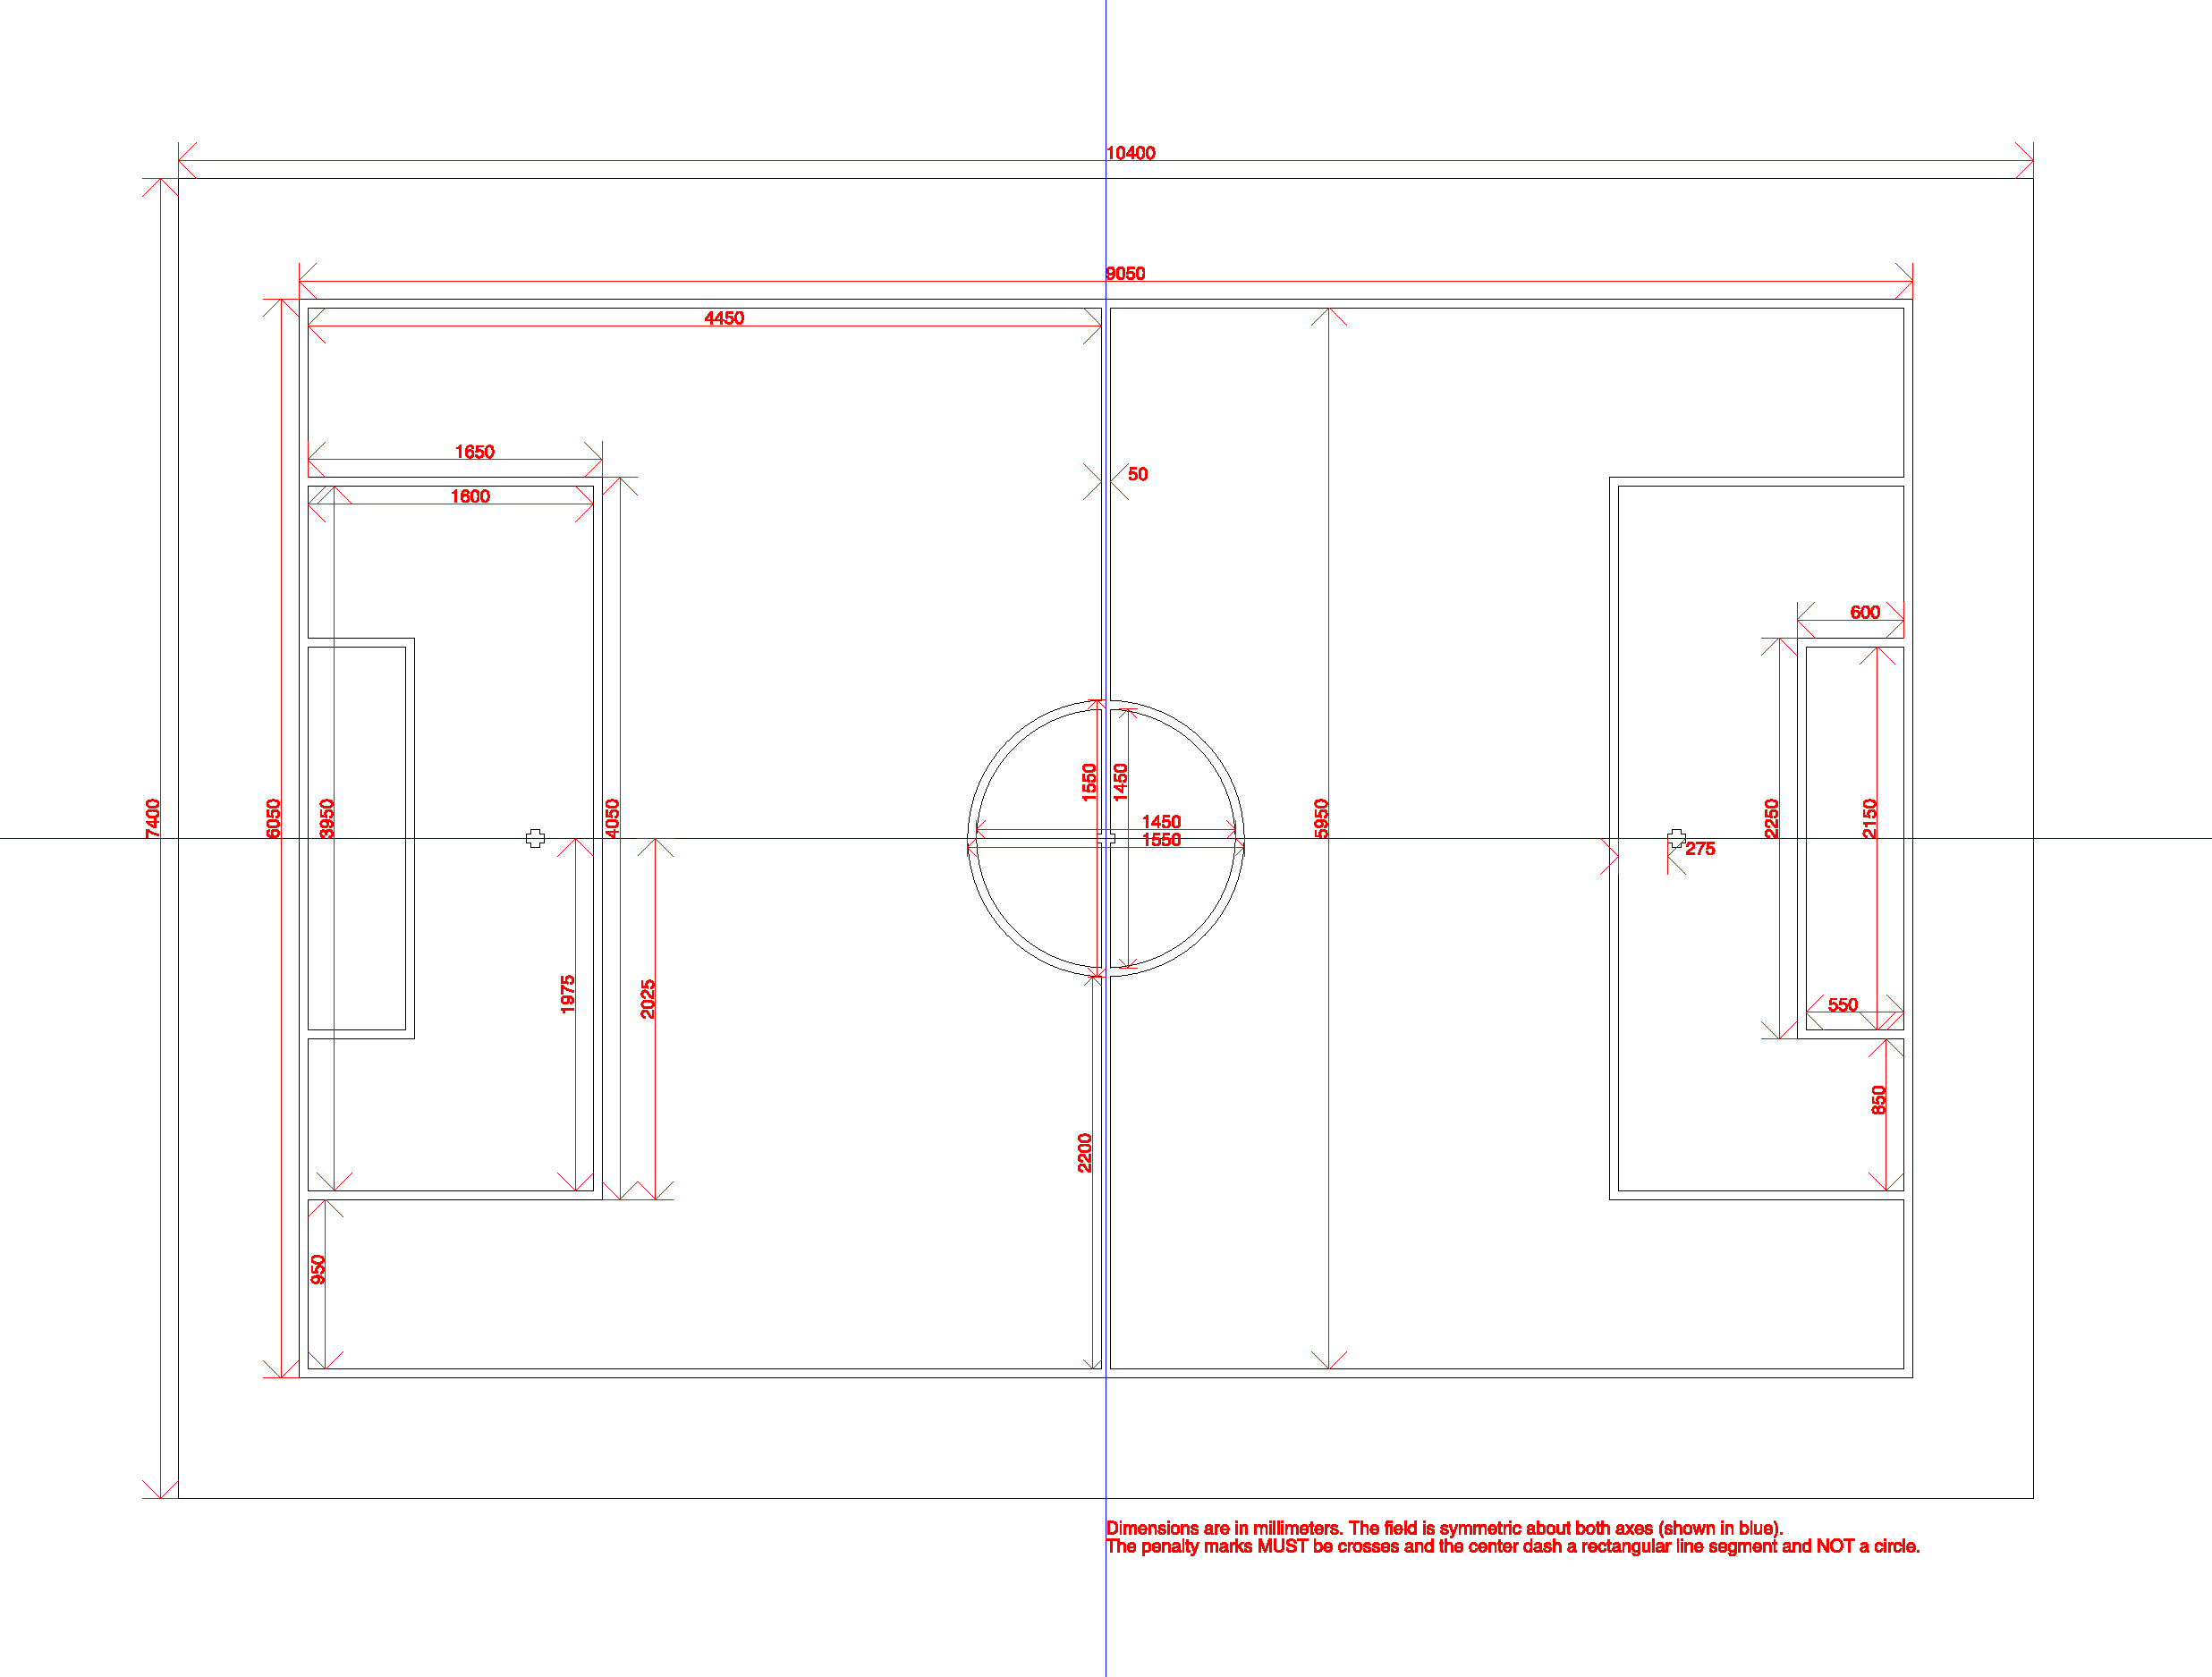
\includegraphics[angle=90,origin=c,width=\columnwidth]{figs/fieldDimensions2020_technical.pdf}}

\clearpage
%\textbf{Center Circle}
\centerline{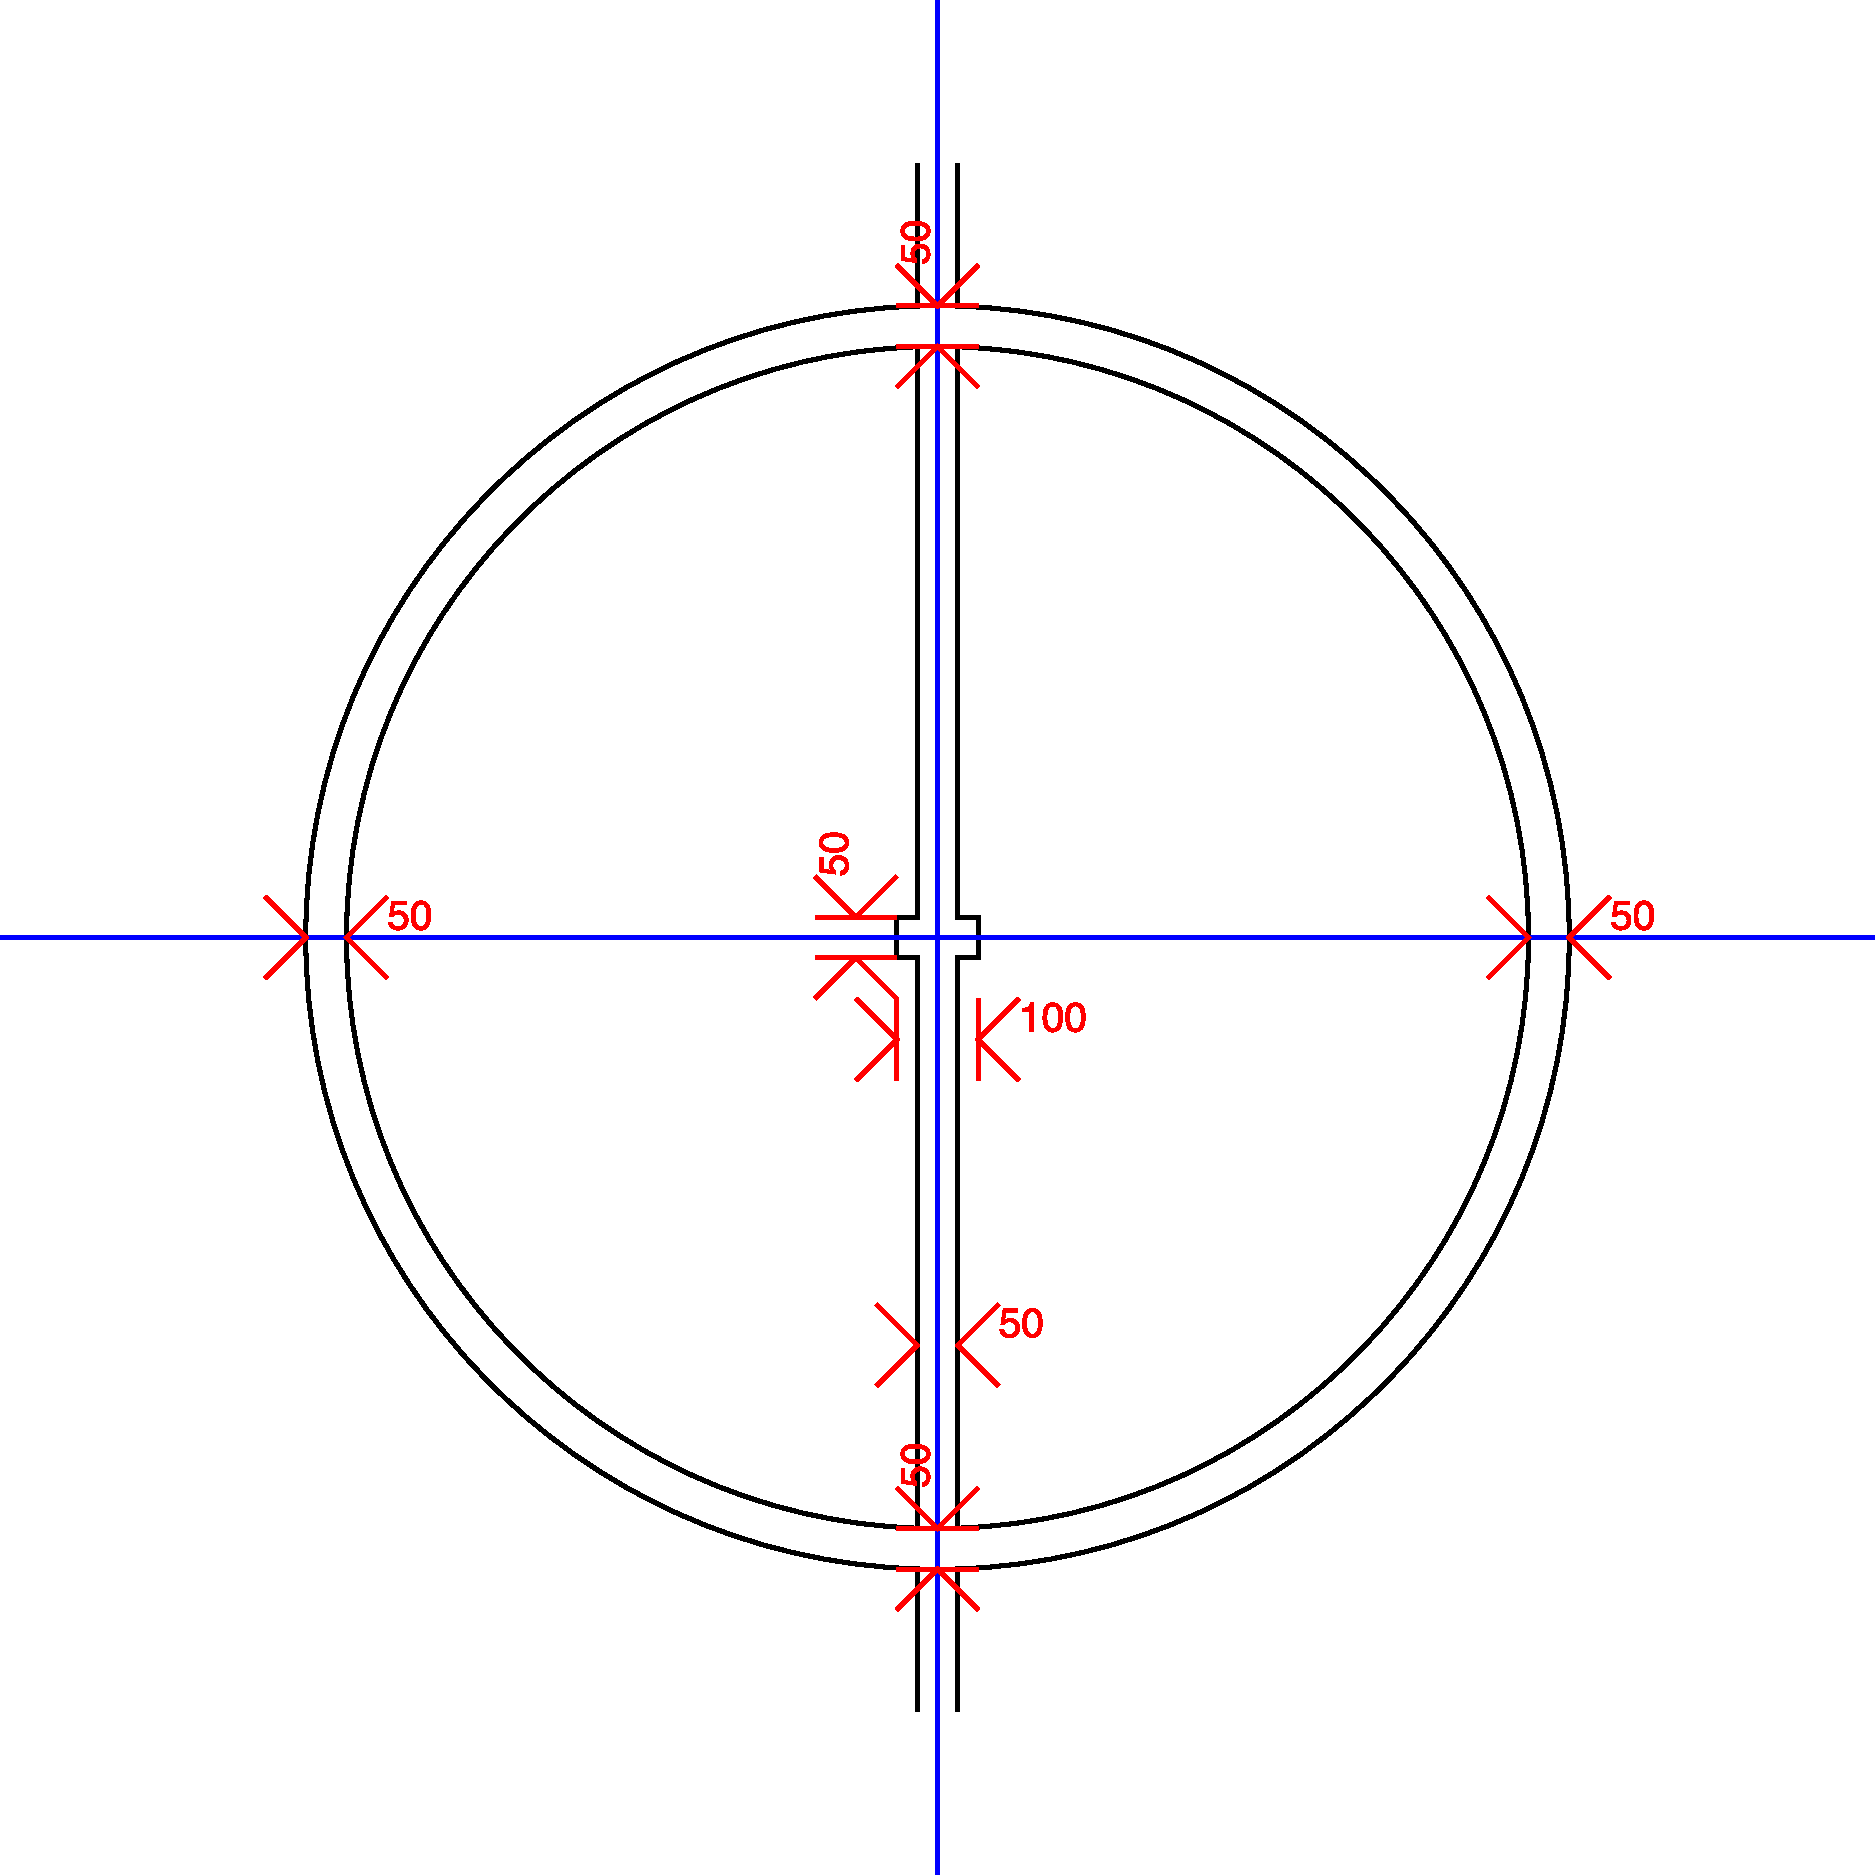
\includegraphics[angle=90,origin=c,width=0.5\columnwidth]{figs/fieldDimensions2020_technical_cc.pdf}}

\centerline{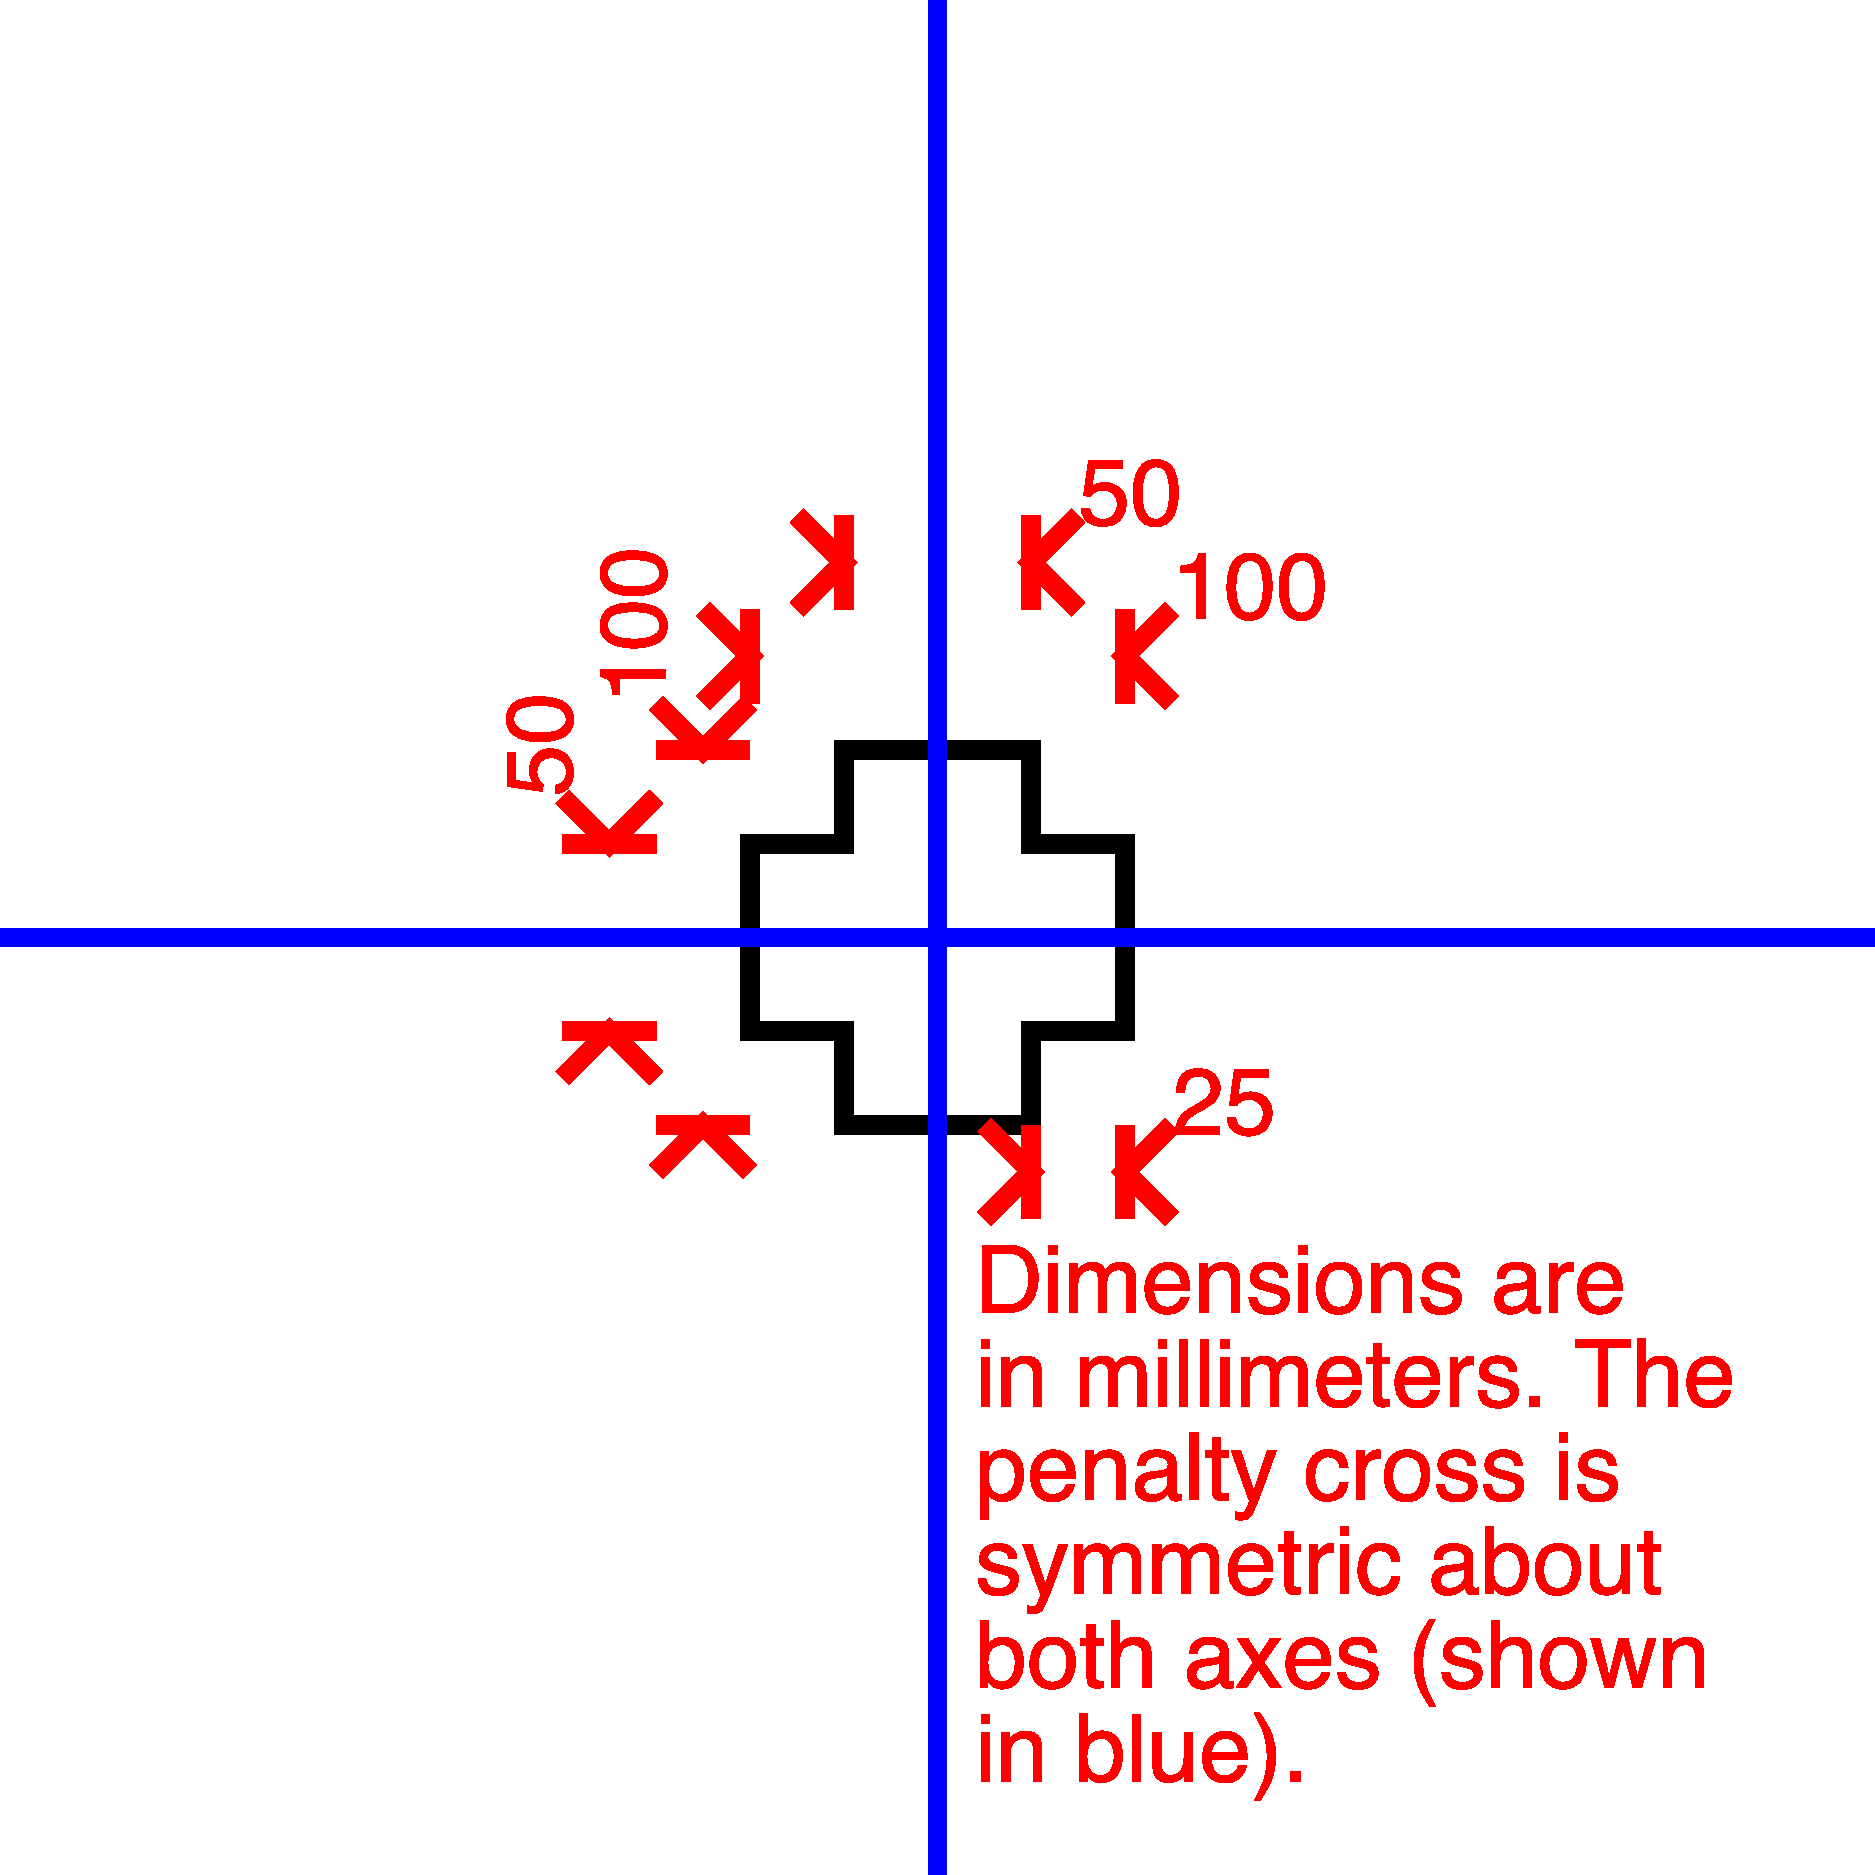
\includegraphics[origin=c,width=0.5\columnwidth]{figs/fieldDimensions2020_technical_pc.pdf}}

%\change{Add the figures for Center Circle and penalty cross as well.}

\end{document}
